%******************************************************************
%******************************************************************
\chapter {Evaluation on Synthetic Data}
\label{experiments}
%******************************************************************
%******************************************************************

In this chapter we perform  systematic experiments on synthetic data, designed to test the performance of optical flow methods.  In the beginning of the chapter we provide a taxonomy of X-ray data. Our classification includes evaluation of image quality, description of data features and artifacts, as well as the description of motion models. Then, we present synthetic datasets, which we employ for our experimental evaluation. Further, we discuss an important aspect of parameters optimization and describe the overall quantitative evaluation procedure.  We present a discussion on the performance, influence of preprocessing, modelling of noise and data outliers and the use of confidence measures. For all the experiments we outline important observations and draw the conclusions, which we summarize in the end of the chapter.


%--------------------------------------------------------
\section{Data Taxonomy}
%--------------------------------------------------------
\label{data_taxonomy}


Since correspondence problems are highly ill-posed and challenging to solve, before any data processing steps are performed, the input data should be systematically evaluated. Its quality, description of the moving objects or the scene, and the motion model should provided a basis for the choice of appropriate data preprocessing routines and optical flow models. Moreover, we emphasize that the clear definition of the application and description of the requirements on the algorithm should be specified. 

One approach to evaluate the data is to perform an explicit quantitative description of the input images. For example, compute a histograms of grey values and velocities, provide the distribution of image derivatives, use noise estimators, etc.
But, it is not always possible to provide such an extensive description - noise estimation can be a difficult task, the motion model prior to the optical flow computation is not known, artifacts are difficult to estimate. In our case we aim to provide a systematic, yet simple and consistent data classification model, which is handy to apply for a wide range of datasets and applications.

In the rest of this section we enlist the most important aspects for our data taxonomy classification. The first category is a description of the image quality.





\subsection{Image Quality}
\textbf{Image Noise}
\\
\\
Noise is a fundamental characteristic of image data. The presence of noise affects the image quality and deteriorates data analysis. To describe the image noise we consider two parameters - the noise model and the amount of noise (or noise level).
\\
\\
\textit{Noise Model}. Is an important characteristic, since it determines the choice of filtering procedure and impose certain requirements on the design of optical flow models. Various noise models that are important for our work are described in Section \ref{noise_models}. 
For our data taxonomy we distinguish the following noise models:
\begin{itemize}
	\item Gaussian noise. This noise model is an approximation model and is frequently used for synthetic datasets in a large body of work on optical flow methods. However, as we have discussed earlier, this model does not adequately describe a physical process of imaging, especially X-ray imaging. 
	
	\item Poisson noise. That is the most important source of noise for X-ray images due to the photon statistics and the detection process. Therefore, it is crucial to test the performance of optical flow methods and the processing techniques on the type of noise.
	
	\item Spike noise. An important noise model to evaluate the performance of computational methods with respect to data outliers.
	
	\item Granular noise. This type of noise is characterized by the varying size and the unknown distribution function. The presence of such noise can be a result of a preprocessing routine, e.g. tomographic reconstruction.
\end{itemize}
Examples of images contaminated with different noise are shown in Figure \ref{fig:noise_models}.
%\comment{Put away this? dont need to give solutions here}To cope with noisy image data two strategies or a combination of them can be employed: use preprocessing step and filter noise from the image data and then proceed with data analysis; use original noisy data as an input for a robust optical flow model. In Section \ref{} we described possible noise filtering methods and in experimental section(s) \ref{}, \ref{} made quantitative evaluation of these techniques.  Based on these experiments we can make the following conclusions: if the amount of noise is small - already a second strategy, i.e. robust optical flow model, can provide good results, otherwise, for high amount of noise - a careful preprocessing step, followed by a robust optical flow computation should be used.
\\
\begin{figure*}[ht]
	
	\centerline{
		\mbox{\includegraphicslabeledw[scale=0.38]{figures/noise_example_poisson.png}{a}}
		\mbox{\includegraphicslabeledw[scale=0.38]{figures/noise_example_spike.png}{b}}
		\mbox{\includegraphicslabeledw[scale=0.38]{figures/noise_example_granular.png}{c}}
	} 
	\caption[]{Examples of X-ray images containing different types of noise. \textbf{(a)} Radiographic image with a large amount of the Poisson noise, as a result of a short exposure time. \textbf{(b)} X-ray image with a good signal-to-noise ratio, but with a substantial amount of the Spike noise (saturated pixels). \textbf{(c)} Radiographic image with the granular noise resulting from a post-processing step of the raw data.}
	\label{fig:noise_models}
\end{figure*}

\textit{Noise Level}. This parameter specifies the amount of noise. As it was already mentioned in the previous section, adequate quantitative estimation of a noise level is a challenging task. Even when such procedure is feasible to perform, it is not clear how to employ this quantitative information to guide the design of processing procedures. For this reason, we omit a measurable estimation of a noise level and proceed with a qualitative, empirical estimation approach. For this purpose we distinguish the following noise levels: 
\begin{itemize}
	\item low: no noise or very little noise is present. In this case no special data treatment is required and design choices for the optical flow model are not restricted to methods that are robust with respect to noise.  
	
	\item average: there is a considerable amount of noise, but the image features are well discernible. A careful consideration of noise is required.
	
	\item high: image data is highly deteriorated with noise. An advanced noise filtering and robust optical flow methods are mandatory to obtain reliable optical flow results.
\end{itemize}

\vspace{0.4cm}
\textbf{Image Contrast}
\\
\\
We refer to the image contrast, as a general ability to distinguish between different image structures. As we already pointed out in Section \ref{contrast_estimation} the contrast-to-noise ratio (CNR) is a more descriptive and useful measure to evaluate the contrast and its implications on the data analysis, then the signal-to-noise ratio or solely image contrast measures.

In the same manner as for the classification of an image noise, we distinguish three contrast levels:
\begin{itemize}
	\item high: there is a pronounced difference in contrast of image features. This includes a high amount of textures and regions with large values of image gradients. This type of datasets is preferred for the  data analysis and usually leads to an accurate optical flow results.
	
	\item average: a contrast is enough to clearly distinguish between features of interest. Moreover, a signal-to-noise ratio for the dataset is acceptable.
	
	\item low: different image features can be hardly distinguished. Additionally, a signal-to-noise ratio is poor, which makes it difficult to enhance the contrast (e.g. using histogram stretching) without augmenting the noisy part of a signal. This case is one of the most challenging image analysis scenarios and an advanced data preprocessing procedure is mandatory to retrieve useful information. 
	 
	  
	
\end{itemize}

Examples of different contrast levels are shown in Figure \ref{fig:contrast_level_examples}.

\begin{figure*}[ht]
	
	\centerline{
		\mbox{\includegraphicslabeledw[scale=0.38]{figures/contrast_example_high.png}{a}}
		\mbox{\includegraphicslabeledw[scale=0.38]{figures/contrast_example_normal.png}{b}}
		\mbox{\includegraphicslabeledw[scale=0.38]{figures/contrast_example_low.png}{c}}
	} 
	\caption[]{Examples of X-ray images with different contrast levels. \textbf{(a)} Radiographic image of aqueous foam with high contrast and good signal-to-noise ratio. \textbf{(b)} Tomographic 2D slice through a \textit{Sitophilus granarius} beetle. The dataset has relatively low contrast between internal structures and poor SNR. \textbf{(c)} Radiographic image of a semi-liquid alloy. Contrast between liquid phase (bright part) and metal particles (dark spots) is very low. Moreover, SNR ratio  is very low.}
	\label{fig:contrast_level_examples}
\end{figure*}

\subsection{Data Features}


%pale green 	#98FB98 	(152,251,152)
%light coral 	#F08080 	(240,128,128)
%lemon chiffon 	#FFFACD 	(255,250,205)


%
%\begin{tabular}{l|c|r}
%  \hline
%  \cellcolor{good}Some & \cellcolor{norm}coloured & \cellcolor{bad}bad \\
%  \hline
%\end{tabular}
%\end{document}


In this section of our data taxonomy we provide a set of parameters to describe a visual appearance of the scene and its objects. Depending on the visual and morphological characteristics of moving objects, different types of optical flow models and their parameters might be optimal. 
In general, all the information about the scene should be identified and described in details. First, this imposes constraints on data constancy assumptions. Second, it describes the requirements for the flow field. Finally, it states the task for the optical flow computation - for which parts of the scene, which dynamical information should be computed. 

Here we list the main aspects of the description of a scene and its objects, that are used in our data classification:
\\
\\
\textit{Object size}.  One of the basic characteristics of an object is its size. The distribution of object sizes may vary a lot within a given dataset. For our classification we are interested to describe extreme values of object sizes, i.e. small and large objects. Additionally, it is important to identify cases, when both categories of objects are present within the same scene.   
Thus, we may distinguish the following categories of object sizes:
\begin{itemize}
	\item small: if the objects of interest are small, a special care should be taken when choosing computational methods and their parameters. For example, if we aim to compute the optical flow on small features, the size of a median mask (See Section \ref{flow_median}) should be adjusted accordingly, since it might eliminate the flow around such small features. In a similar way, the large flow regularization parameters may lead to an oversmoothing of the flow field, resulting in a loss of flow details for small objects.
	
	\item average: by an average size we assume a range of sizes, which do not belong to the extreme values of our categorization approach. In general, such kind of objects do not introduce any restrictions on optical flow models.   
	
	\item large: by a large object we define the object which size exceeds 10-20\% of an image size. In general, the computation of optical flow on large objects should not differ from the objects of average sizes. However, there is an exception. If the object is homogeneous (i.e. contains a small amount of details) and the task is to capture a dense flow field within this object, a large value of the smoothness parameter is required. This can affect the computation in other image regions that contain different data features. That is why the presence of large homogeneous objects should be noted. 
	
	\item mixed: for this case we consider a mixture of small and large objects. This situation is the most challenging, since it requires the simultaneous optimization of parameters for all objects sizes. It is a common problem in the literature that the small image features get smudged because of a significant contribution from the smoothness term. One way to deal with this problem is to use an adaptive smoothness (See Section \ref{adaptive_smoothness}) in different image regions. Another solution is a fusion of results obtained using different model parameters that are specifically tuned for each object category. In any case, a mixture of different objects sizes introduces a major problem for the optical flow computation.   
\end{itemize}

\noindent \textit{Object distribution}. A spatial relationship between objects, i.e. objects density. To describe the object distribution we use the following cases:
\begin{itemize}
	\item sparse: in this situation the objects are distant from each other, separated by a homogeneous background.  Despite the fact that this situation might seem to be easy to handle by optical flow methods, there are some pitfalls. The problem arises from the homogeneous background which separates the objects. In this region there is no contribution from the data term, i.e. aperture problem exists (See Section \ref{general_model}), so the smoothness term takes a lead. As a result, on the boundary between an  object and a background the oversmoothing problem might occur (which depends on the chosen parameter for the flow regularization $\alpha$). And if the object of interest also appears to be details-free, even a larger value of the smoothness parameter is required to precisely capture the motion within such object. In this situation severe oversmoothing artifacts may occur. To summarize, a sparse object distribution can be troublesome in conjunction with the low amount of object details (See next characteristic of object features).
	
	\item normal: this case describes a normal situation for object distribution. Objects might be close to each other or even share a common boundary, but the length of this interface is much smaller, then the perimeter of the corresponding objects. 
	
	\item dense: the objects are close to each other and share substantial amount of their boundaries with other objects. Clearly, in this case a special attention should be paid when choosing optical flow parameters that might lead to imprecise localization of object boundaries. Such parameters include, the gradient constancy assumption as a data term, the presmoothin parameter $\sigma$, the flow regularization parameter $\alpha$, the integration scale $\rho$ and the mask size for the flow median filtering.  
\end{itemize}


\noindent \textit{Object details}. This characteristic describes the amount of image features or details  for the objects of a scene. We distinguish the following quantities of object details:  
\begin{itemize}
	\item low: small amount or no image details (homogeneous objects). For such objects the optical flow computation may be a challenging task and the inappropriate choice of the regularization parameter may lead to oversmoothness artifacts. 
	
	\item normal: this case describes an ideal situation. It means that the amount of image gradients is sufficient to provide enough contribution to the data term. So, no aperture problem exists in most image regions.
	
	\item high: in general, the more details an object has, the more information is available for the data term. However, there might be some exceptions. For example, in \cite{HarmonyFlow} the authors found out that repeating high-frequency image texture can cause aliasing artifacts during the resampling procedure. As a result, the accuracy of optical flow estimation in these regions can be substantially impaired.  Thus, it is important to describe such high-frequency textures and any other periodic structures beforehand.
\end{itemize}


\subsection{Image Artifacts}
\label{image_artifacts}

In this section we present a description of various image artifacts, which affect results of data analysis. All artifacts, if existing, should be treated by an appropriate processing step or computed using a dedicated optical flow model. 
Here we provide a list of possible image artifacts:
\begin{itemize}
	\item \textit{Brightness variations}. Brightness of X-ray images can be non-uniform spatially and non-constant over time (See Figure \ref{fig:artifacts_examples}). Since the main component of every optical flow model is a data term, which imposes certain constancy assumptions on image brightness or other image-based features, the presence of brightness variations is crucial for the design of optical flow models.  
	
	\item \textit{Ring artifacts}. Damaged elements of a detector system cause individual pixels to remain constant during an image acquisition and in particular during the tomographic scanning process. As a result, line structures on sinograms appear. After the reconstruction is performed using the filtered backprojection algorithm these lines form the so-called ring artifacts (See Figure \ref{fig:artifacts_examples}). Such artifacts can significantly deteriorate the accuracy of data analysis. Thus, such artifacts should be removed prior to motion estimation.
	
	\item \textit{Star artifacts}. A non-linear relation between the attenuation coefficient in the material and the intensity values measured by the detector system give rise to the so-called beam-hardening artifacts. These artifacts appear along a geometric path of the respective X-ray beam. After the reconstruction such artefacts appear radially around the boundaries of on object and are called star artifacts (See Figure \ref{fig:artifacts_examples}). Usually, such artifacts are not so pronounced in the region within an object, however, can lead to the incorrect flow estimation on the boundaries of an object. As a possible remedy one can use a dedicated image reconstruction procedure, which is more robust to the beam-hardening artifacts, i.e. algebraic reconstruction techniques with a spatial image regularisation. 
	
	\item \textit{Motion blur}. For the conventional reconstruction methods such as the filtered-back projection, it is assumed that the object is not changing during the acquisition process, so one obtains radiographic projections of the same object from multiple angles. But, this assumption is not always fulfilled. This could be a result of sample motion due to poor experimental conditions, e.g. bad fixation of the sample. Additionally, the motion of a sample could be a part of the experiment, which aims to study dynamical processes. In any case, the inconsistent projection data will result in motion artifacts in the reconstructed volume. The amount of motion blur and the specific steps to take it into account should be described prior to the actual flow computation. 
	
	\item \textit{Projective geometry}. This kind of artifact is characteristic to the radiographic imaging where 3D structures are projected into a 2D detector plane. This effect is similar to the problem of occlusions in the classical optical flow. Such artifacts are non-existing for tomographic data, in which a 3D information about the scene is available. Projective geometry poses a major problem for optical flow computation, since it deteriorates the data constancy assumption.
\end{itemize}

For our data taxonomy, if any of the above mentioned artifacts exists, we mark it as a possible data challenge and provide a list of steps to compensate for it.

%Possible sources of brightness variations:
%\begin{itemize}
%	\item Monochromator stripes (variations)
%	\item Exposure changes
%	\item Changes in sample environment (background)
%	
%\end{itemize}

A list of examples of various image artifacts is shown in Figure \ref{fig:artifacts_examples}

\begin{figure*}[ht]
	
	\centerline{
		\mbox{\includegraphicslabeledw[scale=0.38]{figures/artifacts_examples_bright.png}{a}}
		\mbox{\includegraphicslabeledw[scale=0.38]{figures/artifacts_examples_rings.png}{b}}
		\mbox{\includegraphicslabeledw[scale=0.38]{figures/artifacts_examples_stars.png}{c}}
	} 
	\caption[]{Examples of X-ray images with various image artifacts. \textbf{(a)} Radiographic image of living embryo. Non-uniform brightness variations due to monochromator instabilities. \textbf{(b)} Tomographic 2D slice through a \textit{Xenopus leavis} embryo. Ring artifacts are highly pronounced and severely degrade the image data. \textbf{(c)} Tomographic 2D slice through a weevil incorporated in amber. Note star artifacts due to the beam hardening.}
	\label{fig:artifacts_examples}
\end{figure*}




\subsection{Motion Model}

In order to compute motion one needs to describe which transformations the objects of a scene undergo. In this section we list data properties, which are related to the motion model. We distinguish the following characteristics:
\\
\\
\textit{Motion model}. In general, a motion field is a vector-valued function of spatial coordinates. For practical reasons, it is useful to describe a motion field by means of a simplified model with fewer parameters. The most important motion models for our work are:
\begin{itemize}
	\item translation: the simplest motion model described by a single displacement vector. This transformation preserves the orientation of an object. In most cases this motion model do not pose troubles for the computation of the optical flow.
	\item rotation: is described by the axis of rotation and the angle of rotation. An important aspect of this transformation is that not all data constancy assumptions are invariant under it. For example, gradient constancy assumption, which contains directional information \ref{data_constancy_assumptions}. Clearly, this aspect should be taken into account for the selection of data term.
	\item rigid (translation + rotation): this transformation corresponds to the standard motion model of a rigid body. 
	\item non-rigid: this transformation is not represented by a parametric motion model. Instead, the motion assumed to be local with a certain constraint on its  smoothness (e.g. elastic transformation) or unconstrained at all. 
\end{itemize}

%A summary of 2D transformation is presented in Figure \ref{fig:motion_models} \cite{Szeliski06}.

%\begin{figure*}[ht]
%	
%	\centerline{
%		\mbox{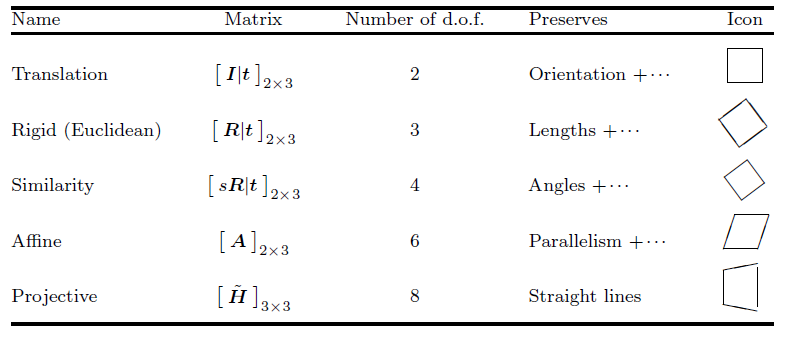
\includegraphics[scale=0.5]{figures/motion_models.png}}
%	} 
%	\caption[]{Hierarchy of 2D coordinate transformations. Image source \cite{Szeliski06}.}
%	\label{fig:motion_models}
%\end{figure*}

\noindent \textit{Motion range}. Another important measure to describe the motion model is to specify the range of velocities with which the objects of the scene move. We distinguish the following motion rates:
\begin{itemize}
	\item small displacement: typically in the range of 1-2 pixels. In this case the linearization of the data term can be performed via the first-order Taylor expansion leading to a convex formulation of the optical flow problem (See Section \ref{general_model}). 
	
	\item large displacement: as soon as large values of object displacements are assumed, we cannot employ linear data terms. This is why an appropriate computation strategy have to be used (See Section \ref{multilevel}). Also the optimal size for the coarsest resolution level is an important factor (See Section \ref{opt_warping_scale}).  
	
	\item mixed: a scenario when both small and large displacements are present and are of interest for the data analysis. For this case, the influence of the  smoothness term should be carefully controlled to preserve small displacements, which tend to be smeared out in the vicinity of a fast motion.
	Additionally, one may consider the adaptive smoothness approach (See Section \ref{adaptive_smoothness}) or a more sophisticated model to respect small movements.
\end{itemize}


\noindent \textit{Motion discontinuities}. It is important to describe the amount of motion discontinuities within a scene. This characteristics plays a key role for the choice of the smoothness constraint. Both spatial and temporal discontinuities should be reported. The following scenarios are important for our data taxonomy:
\begin{itemize}
	\item no discontinuities: for this case we assume a global motion of a scene, described by the same motion model.
	
	\item normal amount: this situation corresponds to a normal case of optical flow computation. There are always discontinuities between objects which are moving with different velocities or directions. Moreover, there is always a motion boundary between the moving object and the static background. It is important to note, that the smoothness assumption is always violated to some extent. The only aim of preserving discontinuities via the appropriate choice of a smoothness term is to allow for piecewise-smooth motion fields.
	
	\item large amount: the cause of discontinuities is the same. i.e. the differences in motion fields, but the amount of flow gradients is large, which requests a particular attention for the choice of a smoothness approach and the corresponding parameters.   
	 
	\item occlusions: in the literature on optical flow methods occlusions between objects or their parts is a major problem. As a result, in the occluded regions not only the information for the data term is lost, but also strong motion discontinuities occur. For X-ray imaging applications occlusions are not present for tomographic datasets, since a 3D information about objects is available. The case when the occlusion problem displays itself is a radiography method, where the projection of 3D structures into a 2D plane gives similar effects. Another important case is the appearance or disappearance of information. This might be a new object entering the scene or formation of a crack in a material, or the process of cell division. For these cases both the data constancy and the motion consistency assumptions are violated.              
\end{itemize}



%--------------------------------------------------------
\subsection{Results Characterization}
%--------------------------------------------------------

To complete our data taxonomy we introduce another important topic - characterization, or requirements, for the output of the  optical flow.
At this point we consider the following important aspects:
\\
\\
\noindent \textit{Accuracy}. No real-life optical flow application should be started without defining the requirements for the accuracy of a result. It can be specified as an upper bound for an average or a maximum error using a chosen error metric (e.g. endpoint error). After the flow field is computed, the results have to be evaluated according to the imposed accuracy limits. This can be achieved by the  comparison with a manual tracking, or using automated confidence measures (See Section \ref{confidence_measures}), or by checking the computed flow with the a-priori information (in the case if motion of some objects is known or can be deduced).   
Verification by visual means may also provide some clues about the accuracy of the computed flow field, but cannot be considered as a reliable way to justify the correctness of the results.  Without specification of error limits and subsequent quantitative verification of the result, the computed flow field cannot be conclusive and trustworthy.            
\\
\\
\noindent \textit{Density}. Specifies whether a dense (i.e. available at every pixel) flow field is required or a sparse representation, available at specified locations is sufficient for the given task. 
\begin{itemize}
	\item sparse: in some cases the requirement on the density of a flow field can be relaxed, which can give a certain degree of freedom to choose model parameters and strategies for the post-processing. For example, one can perform the averaging of the flow vectors from multiple locations or make interpolation of the result using points of high fidelity. These approaches can be especially beneficial for the case of challenging datasets.
	
	\item dense: this is the default scenario for the classical optical flow formulation, where the flow vector is computed for every pixel location.
\end{itemize}

\noindent \textit{Motion components}. Describes which feature of the motion field we are interested to compute. If only one component of the motion field is of relevance, this might give some flexibility to optimize model parameters.
\begin{itemize}
	\item magnitude: if one is interested to estimate the amount of motion, the directional information is not very useful. An example of such scenario is the task of computation of a time-to-impact in driver assistance systems.
	
	\item direction: f one is aimed to estimate directional distribution of the motion field. For this case, the magnitude of the flow field is not relevant.
	
	\item full flow: that is the classical formulation of optical flow, when a flow vector, containing both the direction and the magnitude, is required. 
\end{itemize}


\noindent \textit{Consistancy}. This requirement assumes the consistency of the computed flow field in a forward (between the first image and the second) and backward directions. This condition may be important for various tasks such as image registration and video processing. By the consistency we imply that the flow is the same, but opposite in direction.   
\begin{itemize}
	\item forward: the classical formulation of optical flow, which determines the flow field only in a forward direction.
	
	\item consistent: the motion field, computed in a forward and backward directions should be consistent.
\end{itemize}


\noindent \textit{Motion boundaries}. Before starting optical flow computation it is useful to specify how motion boundaries around moving objects should be treated. Again, this property may be different for various applications. 
\begin{itemize}
	\item strict: Accurate recognition of motion discontinuities is required. In this case a spacial attention should be given to the features of a computation model, which may lead to an oversmoothing or a coarsening of the motion boundaries.
	
	\item not strict: Overall (average) flow is more important and requirements on the precise boundaries estimation are relaxed.
\end{itemize}


\noindent \textit{Computation time}. An important requirement for an optical flow method is the time required to perform the computation. This aspect can significantly influence the choice of an optical flow model, its parameters and the overall accuracy. The requirement is governed by a particular application.       
\begin{itemize}
	\item real-time: for some kind of applications such as driver assistant systems the computation time is crucial. That is why the design of optical flow models is restricted to high-performance methods. 
	
	\item interactive: for some applications the real-time performance is not required, however, some feedback from an user is expected. For instance, if the user wants to inspect the computed flow fields and adjust computation parameters. 
	
	\item offline: for this case there are no limitation on the processing time, so the computation is completely offline. It means that the time complexity of an algorithm is not taken into account and the accuracy of a result is the top priority.
\end{itemize}


\noindent \textit{Data size}. Describes the data size of the input and whether it is possible to process using available memory resources and particular implementation. For the optical flow problem at least two image frames and the flow field should be stored in the memory of a computation unit. For more complex methods, such as a multi-level optical flow (See Section \ref{large_displacements}), motion increments and resampled input images should be additionally stored on each computation level. For some datasets, especially this is typical for a large tomographic volumes, the input data and all variables required for an algorithm, do not fit into the available memory. Thus, the input should be reduced (i.e. using downsampling or cropping), leading to a possible loss of resolution and accuracy. 


%--------------------------------------------------------
\section{Experimental Data}
%--------------------------------------------------------

In order to perform a systematic evaluation of different features of optical flow models, test the results of  data preprocessing routines and investigate the influence of image artifacts, we need to have a set of synthetic test data for which a ground truth result is known.
To obtain such datasets for X-ray images one may proceed in two directions: generate synthetic images exclusively for the X-ray data (see our data taxonomy Section \ref{data_taxonomy}) or, alternatively, one may use the existing datasets and model X-ray related image properties, such as image noise, low contrast and artifacts. 
In this work we proceed with the second approach and use synthetic datasets which are popular in the literature on optical flow methods. Our choice is based on a number of advantages, associated with the second approach. First, these datasets are extensively used and many optical flow methods are already evaluated using them, which makes it easy to compare our results with the previous work. Second, these datasets are publicly available, which can increase the reproducibility of the results. 


  

  

\subsection{Synthetic Datasets}
\label{synthetic_data}

Here we describe synthetic datasets, which we choose for our experimental studies. In total we include three datasets: two datasets depicting a real scenery and one synthetic dataset.

First two image sequences were developed and presented in the work of \cite{Middl}.  The authors made an extraordinary effort to obtain a realistic non-rigid scenes for which a highly accurate optical flow result is available.  In this technique a scene is built from real-life objects and each element of the scene is moved using a mechanical motion stage. The authors applied a fine spatter fluorescent pattern to surfaces of all scene objects. Then, the camera recorded a pair of high-resolution images under the ambient light and the UV illumination (which revealed fluorescent particles). 
The ground truth is obtained by tracking small image blocks in the high-resolution UV images to get integer-valued motion correspondences. As a second step the authors refined the ground truth to the sub-pixel precision using the Lukas-Kanade optical flow algorithm \cite{LucasKanade81}. As a result, a dense ground truth with a verified precision of about 1/10 pixel in the original size and 1/60 pixel in the downsampled size (used as the final result) is obtained.

Here we describe the selected datasets according to our data taxonomy (See Section \ref{data_taxonomy}). 
\\
\\
\textit{RubberWhale} dataset. It contains several independently moving objects, various motion types including non-rigid motion and rotation, different amount of textures.  
Evaluation according to our data taxonomy yields:
\begin{itemize}
	\item \textit{Image noise}: There is no noise in this dataset, perfect imaging conditions.
	
	\item \textit{Contrast level}:  The image contrast is high, the  separation between the objects is good.
	
	\item \textit{Object size}: The scene depicts objects of various sizes, but no small objects are present.
	
	\item \textit{Object distribution}: Objects are distributed normally.
	
	\item \textit{Object details}: Images contain objects with different amount of textures - some of them are highly textured and some of them are more homogeneous. In general, all objects have normal or high amount of details.
	
	\item \textit{Image artifacts}: There are no image  artifacts.
	
	\item \textit{Motion type}: Several types of motion, including translation, rotation, non-rigid motion are present within this dynamic scene. Note, that non-rigid movements (on the blanket, see Figure \ref{fig:gt_images}) vary smoothly, so we do not expect it to cause complications for the optical flow estimation.
	
	\item \textit{Motion range}: Objects are moving with the mixed range of velocities, including slow and fast motion.
	
	\item \textit{Motion discontinuities}: There are occlusions between moving objects, but not very strong ones.
\end{itemize}

\begin{figure*}[!t]
  \centerline{
    \mbox{\includegraphicslabeledw[scale=0.35]{figures/rub1.png}{a}}
    \mbox{\includegraphicslabeledw[scale=0.35]{figures/rub_grounfTruth_bruhn_scale_2px.png}{b}}
  }
  
  \vspace{3pt}
  \centerline{
    \mbox{\includegraphicslabeledw[scale=0.35]{figures/hyd1.png}{c}}
    \mbox{\includegraphicslabeledw[scale=0.35]{figures/hyd_groundTruth_bruhn_scale_2px.png}{d}}
  } 
  \vspace{3pt}
   \centerline{
    \mbox{\includegraphicslabeledw[scale=0.4]{figures/new_marble150.png}{e}}
    \mbox{\includegraphicslabeledw[scale=0.4]{figures/marble_groundTruth_bruhn_scale_2px.png}{f}}
  } 
  
  \caption[]{Synthetic datasets used in the scope of this work for quantitative evaluation of optical flow methods and preprocessing routines. \textbf{(a,b)}  \textit{RubberWhale} dataset. \textbf{(c,d)} \hyd dataset. \textbf{(e,f)}  \mar dataset. Left column: First frame of the corresponding image sequence. Right column:  Ground truth motion field using color code.}
  \label{fig:gt_images}
\end{figure*}
A summary of evaluation of the \rub dataset is given in Table \ref{tab:eval_rub}. The corresponding color codes to classify the influence of certain properties of input data according to our data taxonomy are given in Table \ref{tab:color_codes}.

\begin{table}[ht] \footnotesize
	\centering
	\caption{Color codes to classify the influence of certain properties of input data according to our data taxonomy.}
	\begin{tabular}{ccc}
		\toprule
		\textbf{Color} & \textbf{Description}  \\ 
		\midrule
		\cellcolor{good} good     	    & the feature is advantageous for data processing \\
		\cellcolor{norm} normal     	& in general, the feature should not cause problems  \\
		\cellcolor{bad} challenge     	    & the feature presents a significant challenge \\   
		\bottomrule
	\end{tabular}
	\label{tab:color_codes}%
\end{table}

\begin{table}[ht] \footnotesize
\centering
\caption{Evaluation of \rub dataset.}
\begin{tabular}{ccc}
\toprule
\textbf{Image} & \textbf{Data}   & \textbf{Motion}   \\ 
\midrule
\cellcolor{good} noise: no      	    & \cellcolor{good} size:  average/large  		& \cellcolor{norm}type: vary, non-rigid    \\ 
\cellcolor{good} contrast: high  	& \cellcolor{good} dist: norm     	& \cellcolor{norm} range: mixed  \\ 
\cellcolor{good} artifacts: no       & \cellcolor{good}detail: normal / high 	&  \cellcolor{norm} disc: occlusions   \\ 
\bottomrule
\end{tabular}
\label{tab:eval_rub}%
\end{table}



\textit{Hydrangea} dataset. Contains a large, highly-textured object, which rotates with a fast angular velocity in front of a large background. That background undergoes a translational movement.
Evaluation according to our data taxonomy yields:
\begin{itemize}
	\item \textit{Image noise}: There is no noise in these images, perfect imaging conditions.
	
	\item \textit{Contrast level}:  The image contrast is high, the  separation between the object and the background is good.
	
	\item \textit{Object size}: The scene depicts one object of a large size and large background.
	
	\item \textit{Object distribution}: Only one object is moving in front of the background.
	
	\item \textit{Object details}: The object (a plant) contains a lot of details (leaves). Background is highly textured. Individual leaves, however, have not much details.
	
	\item \textit{Image artifacts}: There are no image  artifacts.
	
	\item \textit{Motion type}: Translational motion of the background. Fast rotation of the object. 
	
	\item \textit{Motion range}: Objects are moving with approximately the same velocity range.
	
	\item \textit{Motion discontinuities}: There is a substantial amount of occlusions around and within the rotating object.
\end{itemize}
A summary of evaluation of the \hyd dataset is given in Table \ref{tab:eval_hyd}.
\begin{table}[ht] \footnotesize
\centering
\caption{Evaluation of \hyd dataset.}
\begin{tabular}{ccc}
\toprule
\textbf{Image} & \textbf{Data}   & \textbf{Motion}   \\ 
\midrule
\cellcolor{good} noise: no      	    & \cellcolor{good} size: large  		& \cellcolor{good} type: rigid, rotation   \\ 
\cellcolor{good} contrast: high  	& \cellcolor{good} dist: norm     	& \cellcolor{good} range: small  \\ 
\cellcolor{good} artifacts: no       & \cellcolor{good} detail: normal / high 	&  \cellcolor{bad} disc: flow discontinuities   \\ 
\bottomrule
\end{tabular}
\label{tab:eval_hyd}%
\end{table}
\\
\\
\textit{New Marble} dataset. It is a computer generated synthetic dataset, which contains two marble blocks moving on a marble floor. This sequence is available at  \url{http://i21www.ira.uka.de/image_sequences/}.
Evaluation according to our data taxonomy gives us:
\begin{itemize}
	\item \textit{Image noise}: There is no noise in these images, the scene is synthetically rendered.
	
	\item \textit{Contrast level}:  The image contrast is high.
	
	\item \textit{Object size}: The scene depicts objects of normal size.
	
	\item \textit{Object distribution}: Normal object distribution.
	
	\item \textit{Object details}: Objects and background  contains a lot of details.
	
	\item \textit{Image artifacts}: There are no image  artifacts.
	
	\item \textit{Motion type}: Translational motion of two blocks, static background. 
	
	\item \textit{Motion range}: Objects are moving with similar velocities.
	
	\item \textit{Motion discontinuities}: There are occlusions around moving objects.
\end{itemize}
A summary of evaluation of the \hyd dataset is given in Table \ref{tab:eval_hyd}.
\begin{table}[ht] \footnotesize
\centering
\caption{Evaluation of \mar dataset.}
\begin{tabular}{ccc}
\toprule
\textbf{Image} & \textbf{Data}   & \textbf{Motion}   \\ 
\midrule
\cellcolor{good} noise: no      	    & \cellcolor{good} size: average  		& \cellcolor{good} type: rigid   \\ 
\cellcolor{good} contrast: high  	& \cellcolor{good} dist: norm     	& \cellcolor{good} range: small  \\ 
\cellcolor{good} artifacts: no       & \cellcolor{good} detail: high 	&  \cellcolor{norm} disc: occlusions   \\ 
\bottomrule
\end{tabular}
\label{tab:eval_mar}%
\end{table}

All dataset are shown in Figure \ref{fig:gt_images}. As it is evident from comparing summary tables for different datasets, the \mar image sequence is the easiest sequence to process in terms of image quality, data features and motion model. On the other hand, the \rub dataset impose more challenges for the optical flow estimation (different motion types, occlusions), and the \hyd dataset is the most challenging in terms of accuracy of the results on the boundaries of the moving object or their parts. Indeed, the inspection of the quantitative results, obtained by the state-of-the-art optical flow methods on these datasets, are in a good agreement with the qualitative estimation based on our data taxonomy. This proves usefulness of our simple, yet adequate approach.    


%Another approach to obtain ground truth datasets is to use manual landmarks or dense motion annotation.
%
%\change{From: \cite{Middl} Most recently Liu et al. (2008) proposed a dataset of real
%imagery that uses hand segmentation and computed flow estimates
%within the segmented regions to generate the ground
%truth. While this has the advantage of using real imagery,
%the reliance on human judgement for segmentation, and on a
%particular optical flow algorithm for ground truth, may limit
%its applicability.}


%Fixed parameters (optimized for maximum performance on the original data):
%
%\begin{table}
%\begin{center}
%  \begin{tabular}{ l || c | r }
%    \hline
%    dataset & $\alpha$ & $\sigma$ \\ \hline
%    rub & 1.6 & 0.15 \\ \hline
%    hyd & 3.4 & 0.15 \\ \hline
%    mar & 3.5 & 0.15 \\ 
%    \hline
%  \end{tabular}
%  \label{tab:test}
%  \caption{A normal caption}
%\end{center}
%\end{table}


\subsection{Modeling Properties of X-ray Data}
\label{modeling_xray_data}

In the current work to test the performance of data processing routines, choose the appropriate optical flow models and their parameters we use synthetic data for which the ground truth result is known. In this way we have a possibility to perform an extensive quantitative evaluation of the devised techniques and deduce sound conclusions.  To achieve that we use synthetic datasets which are popular in the literature on optical flow methods, are publicly available, and extensively studied. As the next step we simulate all X-ray data related image properties, which account for different imaging scenarios. Note, that we do not aim to produce realistically looking synthetic X-ray datasets, however, such work could be useful. In this section we show our approach to model the most important properties of the X-ray data, which are image noise, low-contrast, illumination changes, and image artifacts.


\subsubsection{Image Noise}
\label{modeling_image_noise}

To perform experiments under different noise conditions we choose three noise models presented in Section \ref{noise_models}.
We start our evaluation with a \textit{Gaussian} model, which is a popular choice to introduce noise artifacts. Then we proceed with a more physically justified noise model - \textit{Poisson} noise. It is important to compare how the Gaussian and the Poisson noise models are differ and which implication it makes on the design of the robust optical flow techniques.
Then, we use a very specific \textit{Spike} noise model that aims to emulate the presence of data outliers, potentially caused by dead and saturate pixels. 
Here we describe which parameters and implementations we use to model image noise:

\begin{itemize}
	\item \textit{Gaussian noise}. For the implementation of
	 the Gaussian noise we used a plugin for an open-source ImageJ/Fiji software \cite{Schindelin12, Schneider12} called RandomJ, which is freely available at the website: \url{http://www.imagescience.org/meijering/software/randomj/}. We vary standard variation $\sigma$ to achieve different noise levels. An example of images contaminated with the  Gaussian noise is shown in Figure \ref{fig:noisy}.
	
	\item \textit{Poisson noise.}  For the implementation of photon noise according to the Poisson distribution we used the same plugin as for the Gaussian noise. To produce images with different level of Poisson noise we use different values of the mean value of the Poission distribution $\mu$.
	
	\item \textit{Spike noise}. For the implementation of the Spike noise we  used an open-source ImageJ/Fiji software \cite{Schindelin12, Schneider12}. By default the percentage of corrupted pixels affected by the routine is 5\%. To increase the amount of noise we run the method multiple times. 
\end{itemize}


On Figure \ref{fig:noisy} we show an example of \rub dataset contaminated with the \textit{Gaussian} noise. Histograms obtained from images with different noise levels reveal dramatic changes in the pixels content caused by noise. To check the performance of optical flow methods on images with varying amount of noise and accuracy of the results depending on the noise level we run a simple experiment on all three datasets. We vary use the Gaussian noise model and vary the standard deviation parameter. For all datasets we show the average endpoint error (AEE) in three regions: for the whole image domain (\textit{All}, on motion discontinuities and within the homogeneous image regions (\textit{Untext}). The evaluation results are shown in Figure \ref{fig:noise_evaluation}. From these plots and inspection of the quantitative results we can make the following observations and conclusions:

\begin{itemize}
	\item The \mar dataset is the simplest among our testing dataset and the optical flow computation gives best results. Both errors in \textit{All}, as well as in \textit{Disc} and \textit{Untext} regions are the smallest. In turn, the \rub and \hyd datasets are much more challenging to process. Our data taxonomy allowed to predict such results, since it highlights the characteristic properties of each dataset. Thus we, again, make certain that our approach is practical.
	
	\item The performance of optical flow methods on all datasets is quite different, both in terms of accuracy, as well as in influence of noise on the final result. For example, for \rub and \mar datasets, the dependence is more or less linear. For \hyd dataset more interesting behaviour takes place (see next). This confirms the rationale behind our data classification - every dataset should be carefully analysed and treated with the optimum algorithm and parameters.
	
	\item As it can be expected, the performance in various image regions is different. The most complicated cases are regions around object and motion discontinuities. However, this also depends on the noise level and original contrast of the input sequence. For example, for \hyd dataset for noise levels more then $\sigma=12$  in the region of homogeneous background, high amounts of noise results in a incorrect motion estimation and this becomes the dominant contribution to the overall error.
		
	\item There is a substantial statistical variability in the results depending on the concrete noise distribution. Note, that in some cases the results on images with higher amount of noise are more accurate then on images with lower amount of noise. This means that for the evaluation of noise it is not enough to make conclusions from a single noise dataset. Instead, statistical measurements should be performed. As a result, such measurement should include statistically sufficient number of experiments and report the average value and the standard deviation as a result.   
\end{itemize}

 


\begin{figure*}[!ht]
  \centerline{
    \mbox{\includegraphicslabeledw[scale=0.25]{figures/hyd1_n00.png}{a}}
    \mbox{\includegraphicslabeledw[scale=0.25]{figures/hyd1_n20.png}{b}}
    \mbox{\includegraphicslabeledw[scale=0.25]{figures/hyd1_n40.png}{c}}
  }
  \vspace{3pt}
   \centerline{
    \mbox{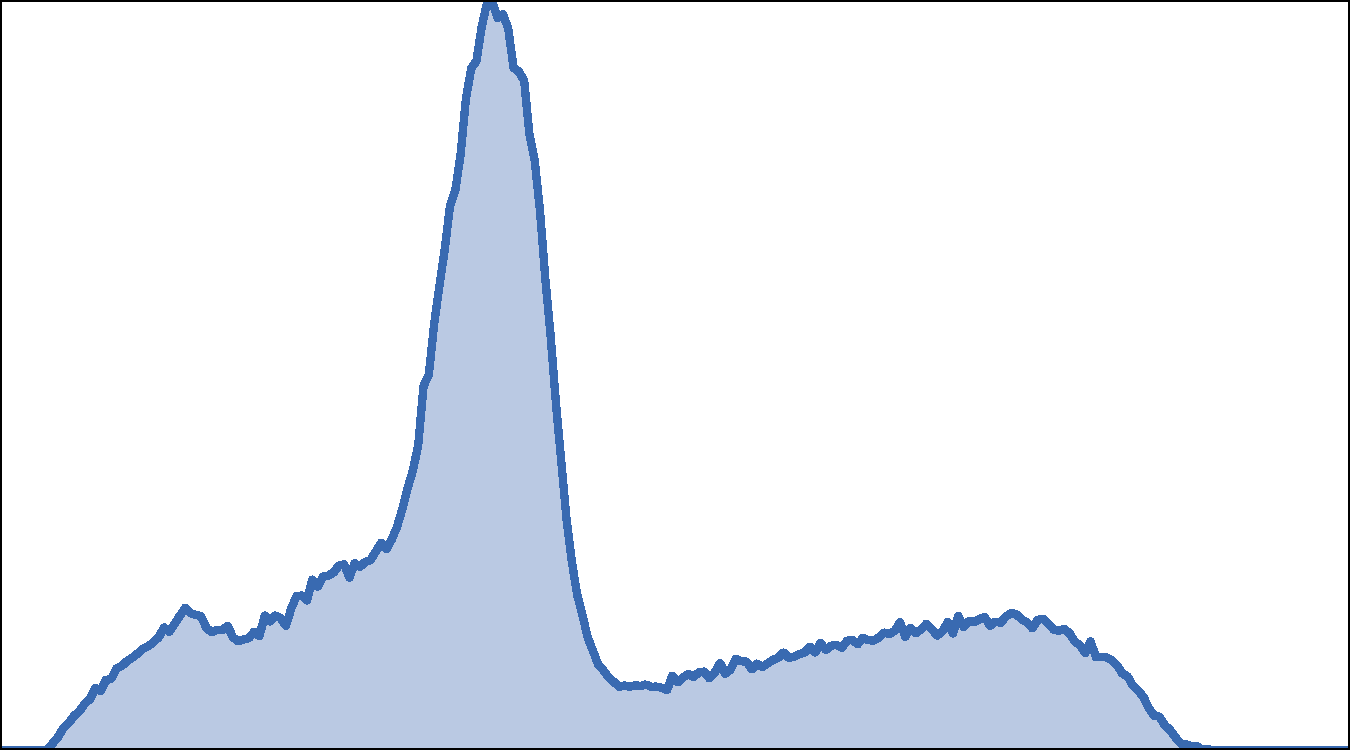
\includegraphics[width=0.3215\textwidth]{figures/hyd1_n00_hist.pdf}}
    \mbox{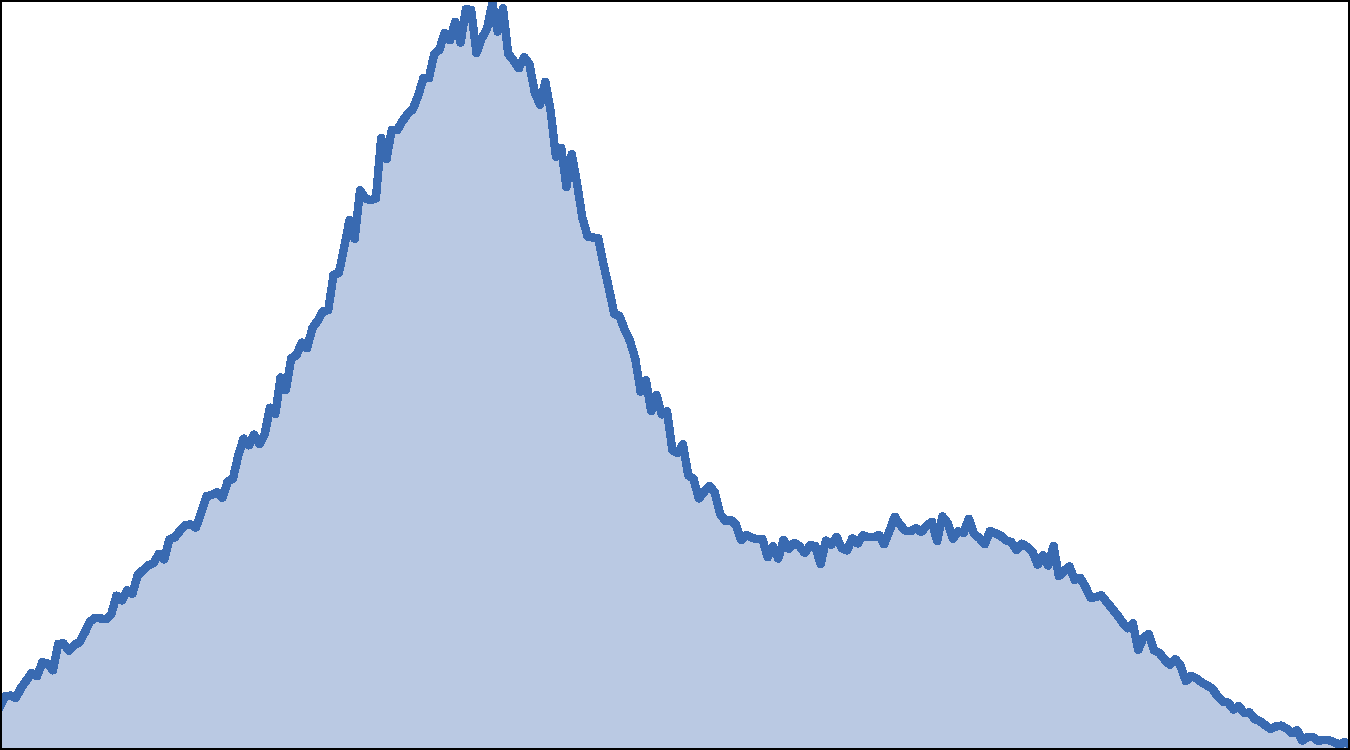
\includegraphics[width=0.3215\textwidth]{figures/hyd1_n20_hist.pdf}}
    \mbox{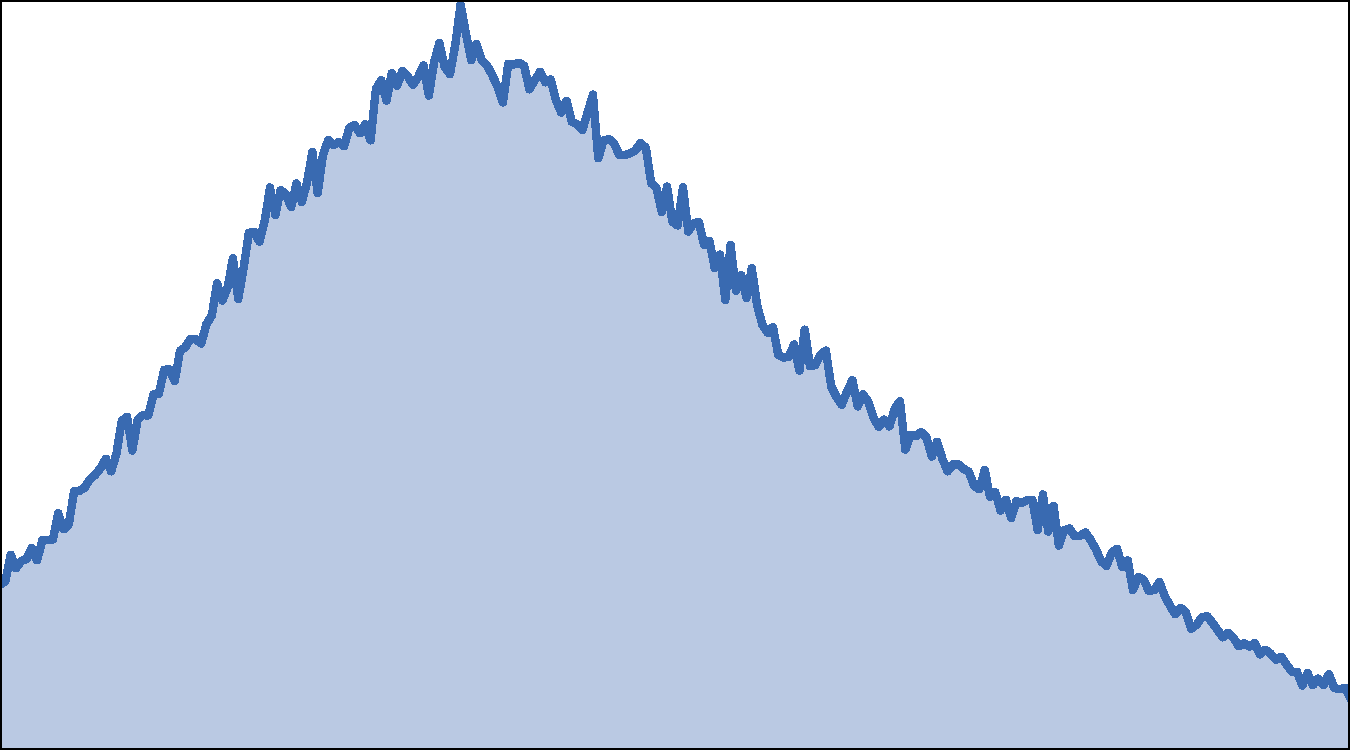
\includegraphics[width=0.3215\textwidth]{figures/hyd1_n40_hist.pdf}}
  }
  
  \centerline{
     	\mbox{
\includegraphics[scale=0.565]{figures/hist.png}}
     	\mbox{
\includegraphics[scale=0.565]{figures/hist.png}}
     	\mbox{
\includegraphics[scale=0.565]{figures/hist.png}}
  }
  \caption[Modeling noisy datasets]{Modeling noise for the \hyd dataset using the \textit{Gaussian} noise model. \textbf{(a)} First frame of the original image sequence. \textbf{(b)} Image with added Gaussian noise with standard deviation $\sigma = 20$. \textbf{(c)} Image with added Gaussian noise with standard deviation $\sigma = 40$. \textbf{Bottom Row:} Corresponding histograms. Note a dramatic change in the grey value distribution as a result of noise.}
  \label{fig:noisy}
\end{figure*}




\begin{figure*}[h]
%  \centerline{
%    \mbox{\includegraphics[scale=1.0]{figures/plot_noise_level_evaluation.png}}
%  }
    \centering
    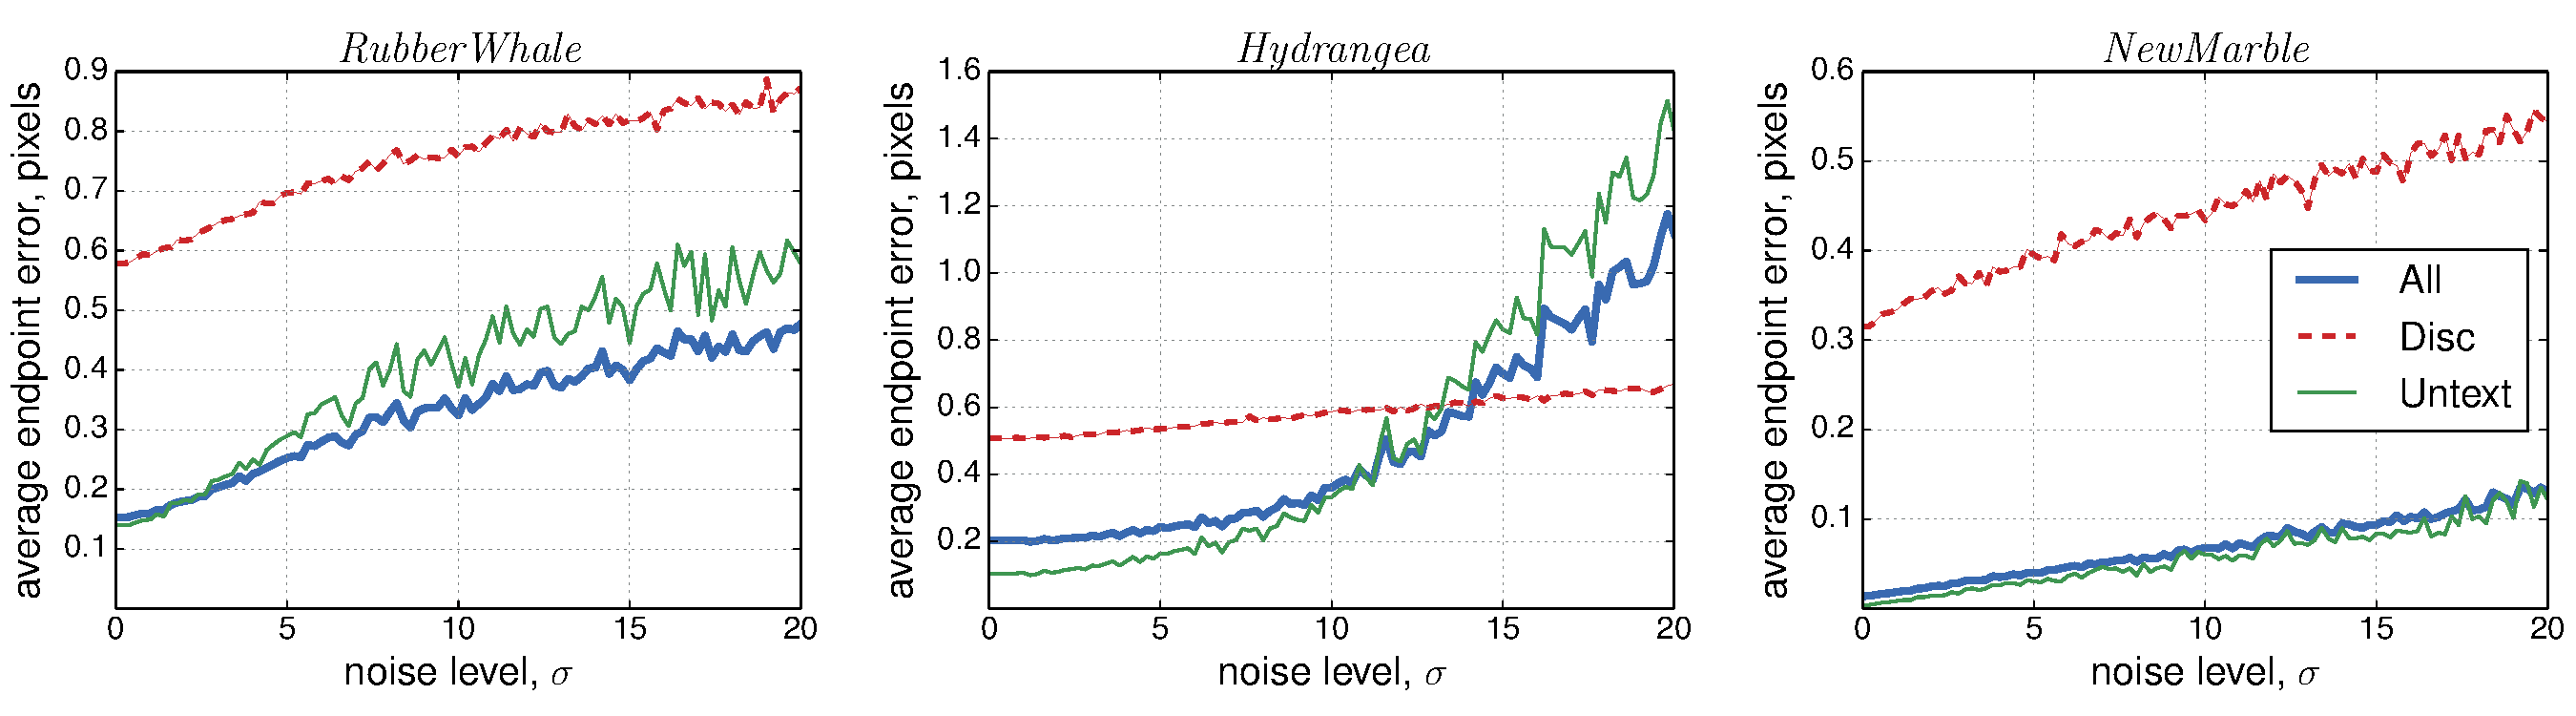
\includegraphics[width=\textwidth]{figures/exp_noise_comp_3_datasets.pdf}
  
  \caption[Noise evaluation]{Evaluation of optical flow performance on noisy data with \textit{Gaussian} noise. For all datasets an average endpoint error (AEE) is shown in 3 regions: \textit{All} region is depicted as a green plot; \textit{Untext} region as a blue plot and \textit{Disc} region as a red plot.  \textbf{Left:} \rub dataset. \textbf{Middle:} \hyd dataset. \textbf{Right:} \mar dataset. Method: \textit{Baseline} algorithm (See Section \ref{baseline_method}).}
  \label{fig:noise_evaluation}
\end{figure*}


Datasets with synthetically added noise will be used for the quantitative evaluation in the following sections :
\begin{itemize}
 \item In Section \ref{experiment_noise_reduction} to show how noise affects the performance of \opticalflow and to evaluate different noise reduction approaches presented in Section \ref{contrast_adjustment}.
 
 \item In Section \ref{experiment_data_terms_for_noisy_data} to make a comparison between simple and higher-order data constancy assumptions and draw the conclusions about which of them are more robust w.r.t. to noisy data.
 
 \item In Section \ref{experimen_combined_local_global_approach} we evaluate the influence of incorporating the local information into the data term (CLG approach).
 
 \item In Section \ref{experiment_normalization_data_term} we study the result of data normalisation and its implication on the accuracy of flow computation.
 
\end{itemize}

 

\subsubsection{Contrast Level}
\label{model_contrast_level}

Another important property to evaluate is contrast. Since the X-ray data exhibits a wide range of image contrast levels (depending on imaging parameters), it is crucial to simulate and estimate the influence of image contrast on the performance of \opticalflow methods. 

To implement various contrast levels we take the original image sequence and reduce the contrast via the histogram rebinning while keeping the original values of maximum and minimum of the original histogram. An example of contrast reduction is illustrated in Figure \ref{fig:contrast_level}. 


%\change{Additionally, we estimate the performance of OF on such a image quality metric as Contrast-to-noise ratio and argue that such characteristics is very important while working with X-ray images.}

\begin{figure*}[!ht]
  \centerline{
    \mbox{\includegraphicslabeledw[scale=0.25]{figures/hyd1_c_000.png}{a}}
    \mbox{\includegraphicslabeledw[scale=0.25]{figures/hyd1_c_100.png}{b}}
    \mbox{\includegraphicslabeledw[scale=0.25]{figures/hyd1_c_200.png}{c}}
    }   
     \vspace{3pt}
   \centerline{
   	\mbox{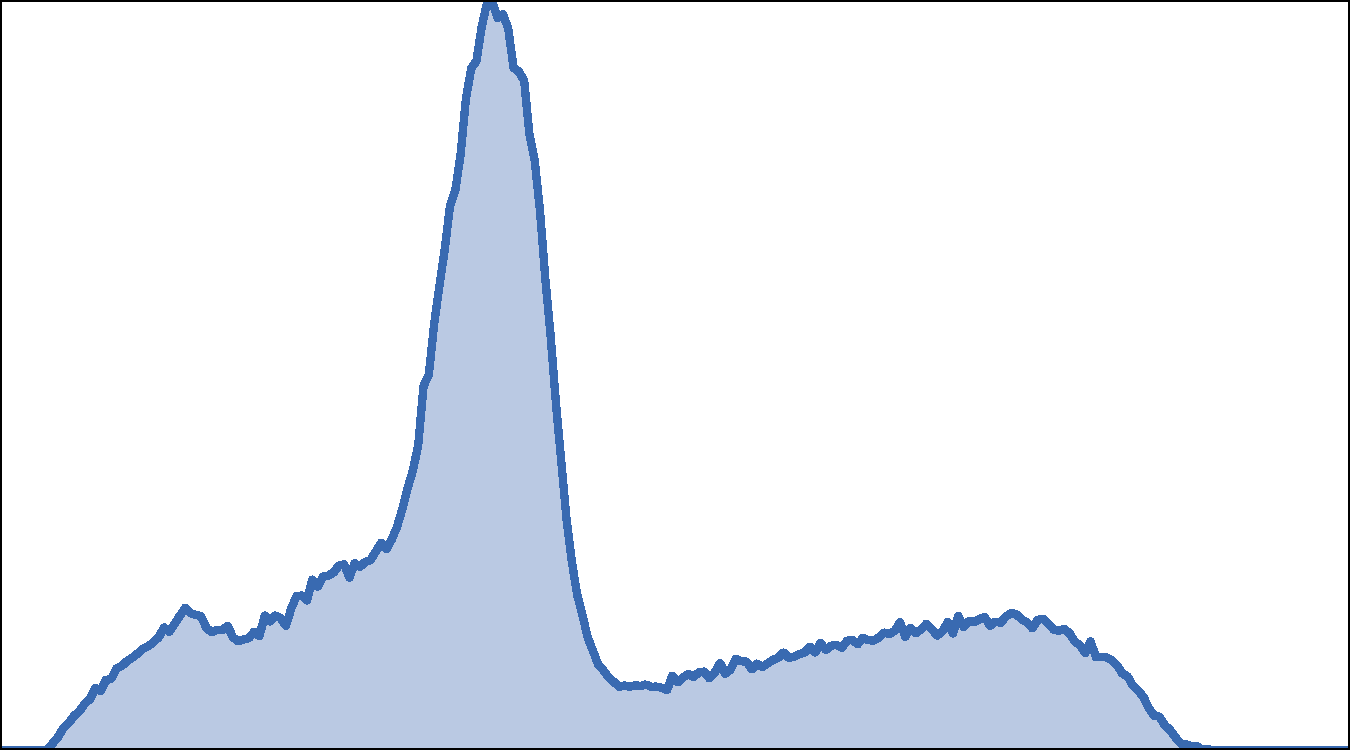
\includegraphics[width=0.3215\textwidth]{figures/hyd1_n00_hist.pdf}}
   	\mbox{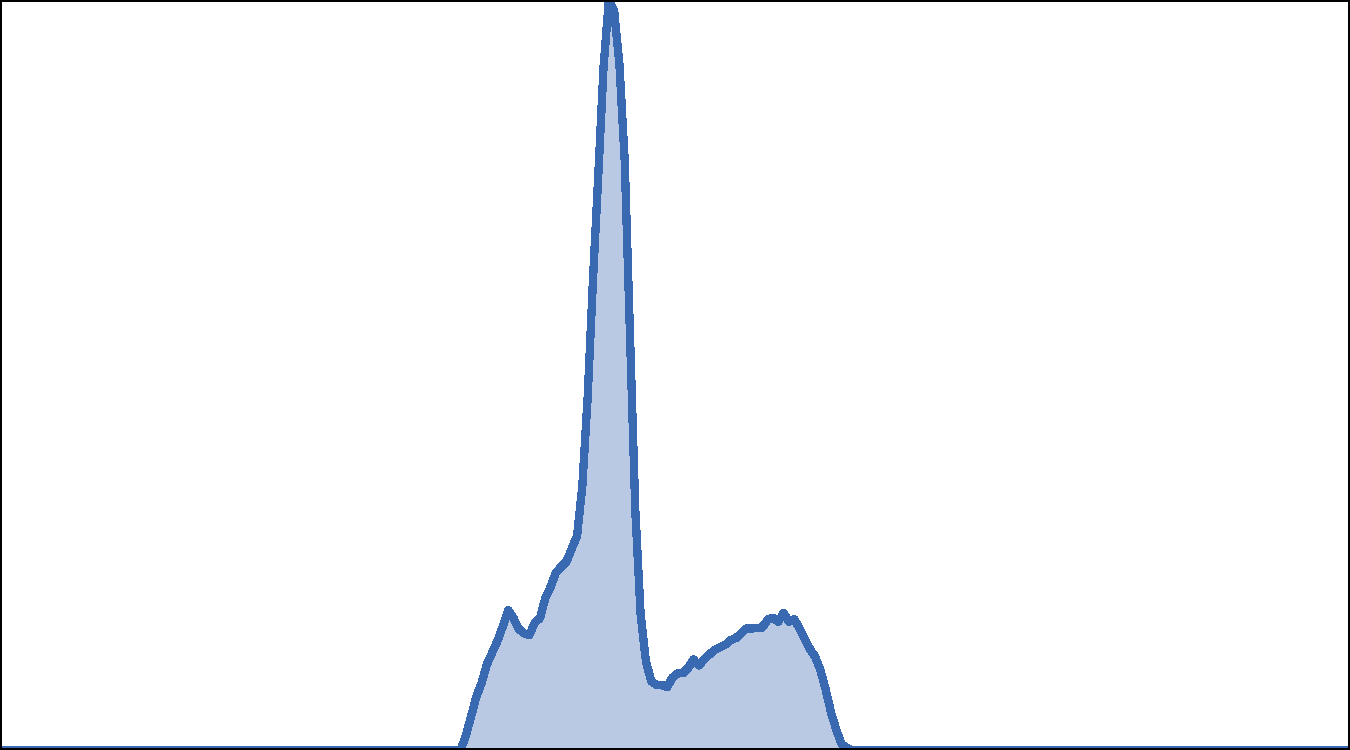
\includegraphics[width=0.3215\textwidth]{figures/hyd1_c_100_hist.pdf}}
   	\mbox{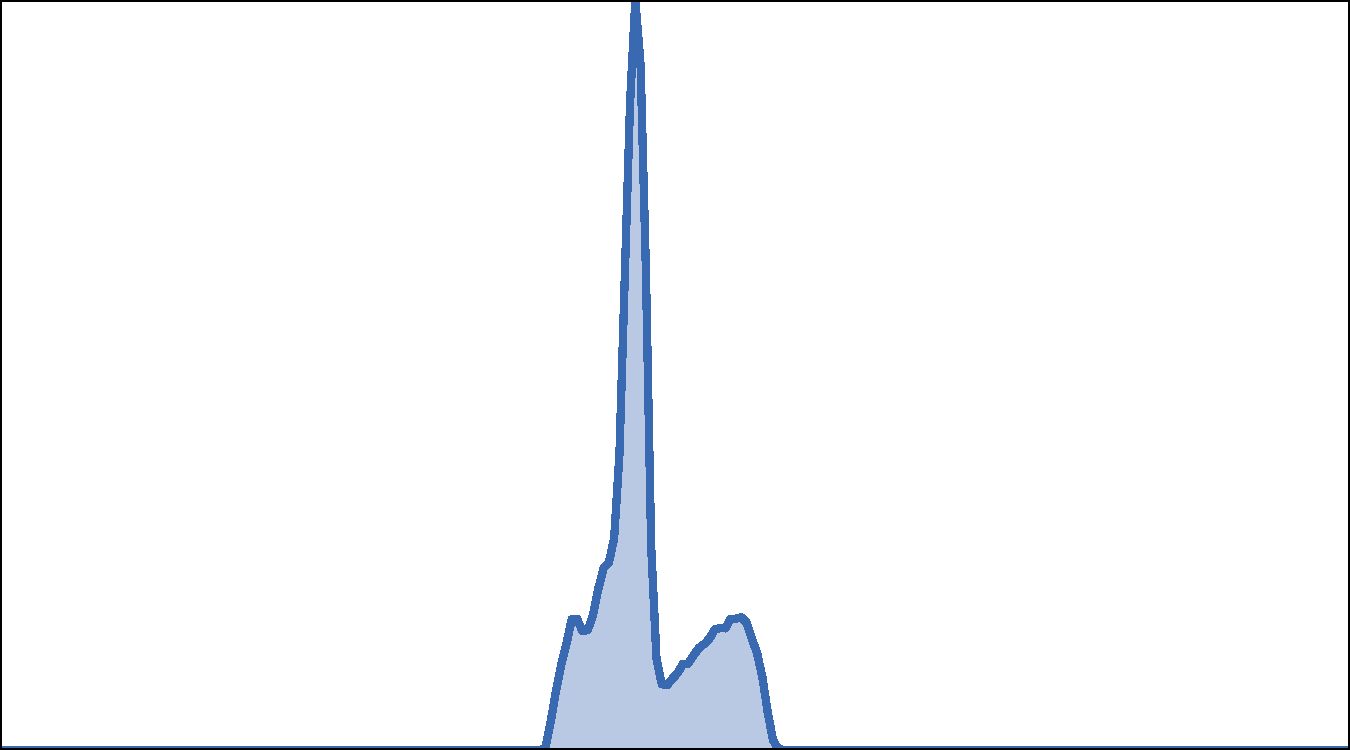
\includegraphics[width=0.3215\textwidth]{figures/hyd1_c_200_hist.pdf}}
   }
   
   \centerline{
   	\mbox{
\includegraphics[scale=0.565]{figures/hist.png}}
   	\mbox{
\includegraphics[scale=0.565]{figures/hist.png}}
   	\mbox{
\includegraphics[scale=0.565]{figures/hist.png}}
   }
  \caption[Modeling contrast]{Modeling datasets with low feature contrast. \textbf{(a)} First frame of the original sequence. Contrast level $C = 100\%$. \textbf{(b)} Image with the reduced contrast.  Contrast level $C = 25\%$. \textbf{(c)} Contrast level $C = 12.5\%$. \textbf{Bottom Row:} Corresponding histograms showing a reduction in the dynamic range and, as a result, in the contrast level.}
  \label{fig:contrast_level}
\end{figure*}

To justify the importance of investigation of contrast changes on the results of motion estimation we perform an experiment in a similar fashion as we did with the previous experiment. We take a fixed optical flow model (\textit{baseline} method) and evaluate its performance on the images with different contrast values, varying it from $100\%$ of contrast to $7.5\%$. The evaluation plots are shown in Figure \ref{fig:noise_evaluation}.
Analysing them we can make the following conclusions:
\begin{itemize}
	\item The shrinkage of the dynamic range and a loss of useful information causes a severe degradation of the accuracy of optical flow results. For the substantial decrease in contrast the performance drop is significant and can be compared with the influence of noise. That is why even for low noise image data, an appropriate adjustment of computation parameters is required. 
	
	\item \hyd dataset contains a large amount of textural information in all image regions, as a result it is the easiest dataset to process, even in the case of low-contrast data.
	
\end{itemize}




\begin{figure*}[h]
%  \centerline{
%    \mbox{\includegraphics[scale=1.0]{figures/plot_noise_level_evaluation.png}}
%  }
    \centering
    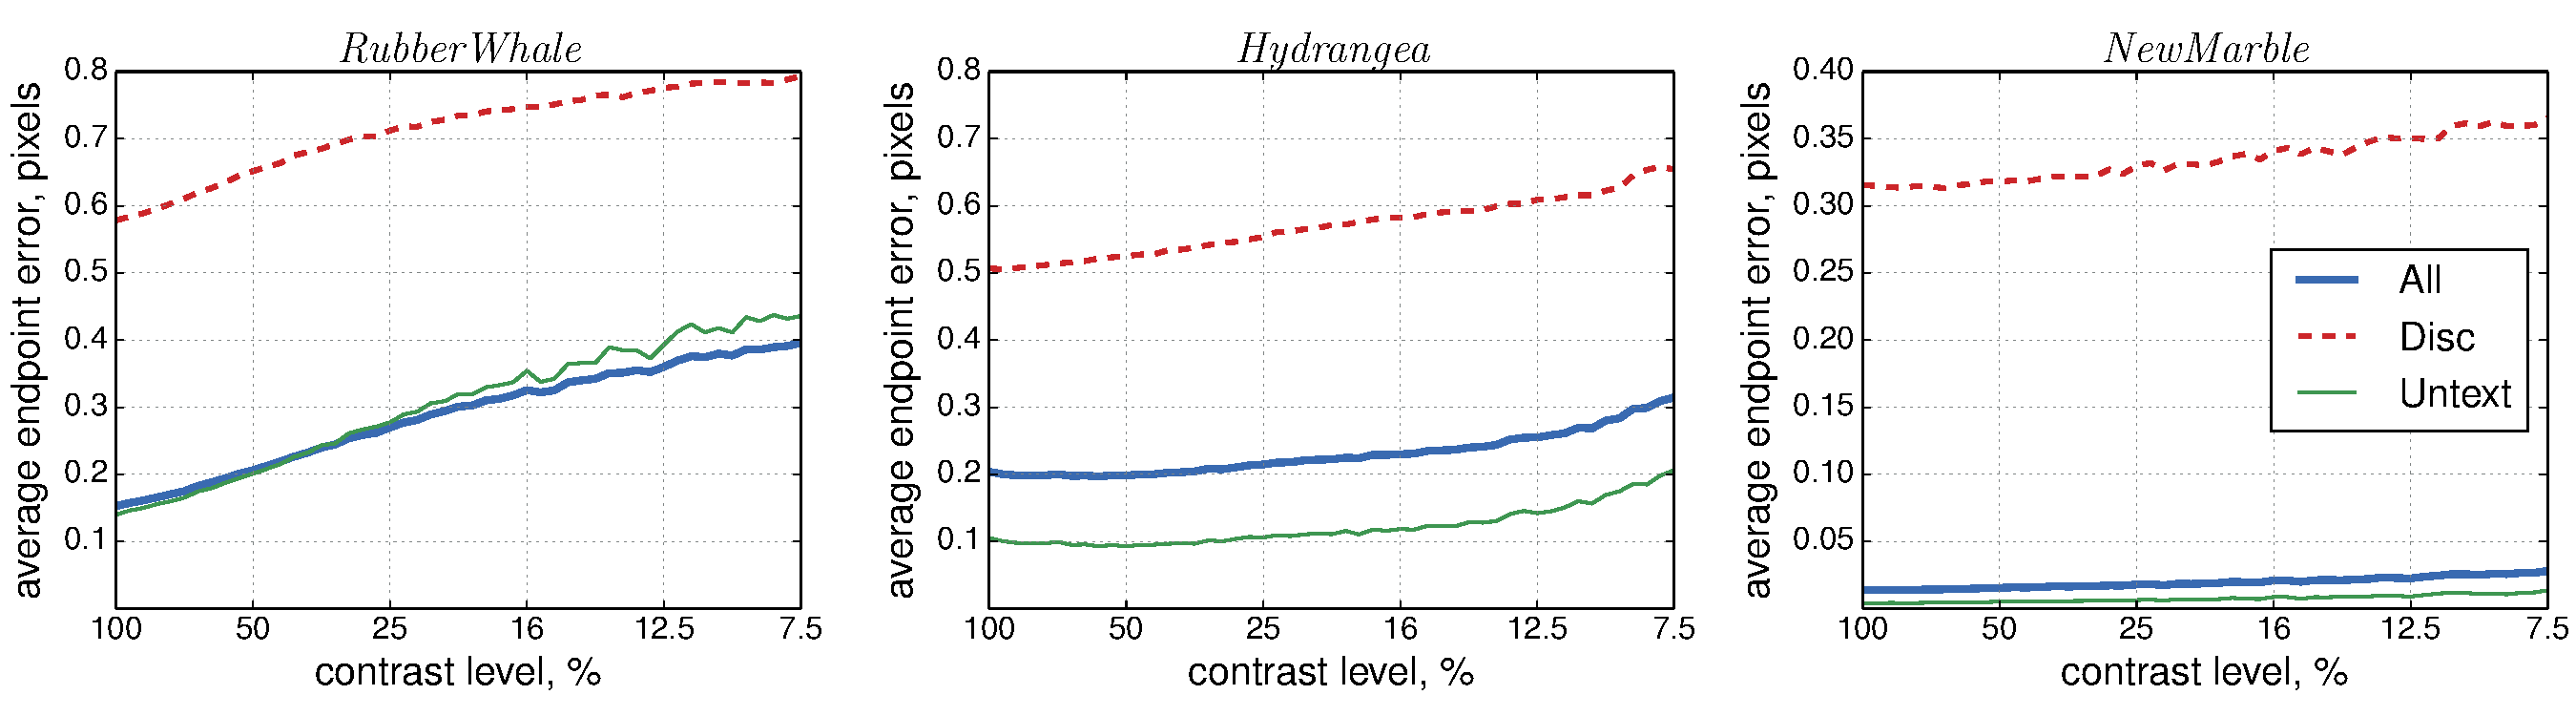
\includegraphics[width=\textwidth]{figures/exp_contrast_comp_3_datasets.pdf}
  
  \caption[Fixed vs Optimal]{Evaluation of optical flow performance on 
 datasets with degraded  contrast level. For all datasets an average endpoint error (AEE) is shown in 3 regions: \textit{All} region is depicted as a green plot; \textit{Untext} region as a blue plot and \textit{Disc} region as a red plot.  \textbf{Left:} \rub dataset. \textbf{Middle:} \hyd dataset. \textbf{Right:} \mar dataset. Method: \textit{Baseline} algorithm.}
  \label{fig:contrast_evaluation}
\end{figure*}

We will use the datasets with the low-contrast in the following experiments:
\begin{itemize}

 \item In Section \ref{experiment_local_contrast} to show how a decrease in the image contrast affects the performance of \opticalflow, as well as to evaluate different contrast enhancement  approaches presented in Section \ref{contrast_adjustment}.
 
  \item In Section \ref{experiment_data_terms_for_contrast_data} to check the performance of different data terms, make comparison between them and draw conclusions about the data terms which are more robust with respect to low-contrast data.

  \item In Section \ref{experiment_robust_data_term_low_contrast} to evaluate the influence of robustification of the data term for low contrast image data.
 
\end{itemize}



\subsubsection{Brightness Changes}
\label{modeling_brigntenss}

In this section we describe different types of illumination changes, which may occur in X-ray data. Since the assumptions about brightness distribution of the scene and objects is the core information for the construction of data terms, any changes in brightness or illumination are important to take into account for the design of optical flow model or data preprocessing.

In this work we consider the following models of illumination changes:
\begin{itemize}
  \item Global additive illumination. For this case a constant value of $A$ is added to every pixel of the second image of the input sequence.
  \item Global multiplicative illumination. Every pixel of the second image frame is multiplied by a factor $M$. It is important to note, that changes in exposure time are corresponding to global multiplicative brightness change, thus is very important to model.
  \item Smooth spatial variation. We consider two patterns:  \textit{"Spot"}, resembling changing beam spot and \textit{"Strips"} pattern, simulating horizontal brightness flickering due to instability of a monochromator.
\end{itemize}

Two spatial patterns intended to simulate the uneven brightness distribution are presented in Figure \ref{fig:patterns}.

\newcommand{\patternsSize}{0.25}

\begin{figure*}[!ht]
  \centerline{
    \mbox{\includegraphicslabeledw[scale=\patternsSize]{figures/rub1.png}{a}}
    \mbox{\includegraphicslabeledw[scale=\patternsSize]{figures/rub2.png}{b}}
    \mbox{\includegraphicslabeledw[scale=\patternsSize]{figures/diff_original.png}{c}}
  }
  \vspace{3pt}
  \centerline{
    \mbox{\includegraphicslabeledb[scale=\patternsSize]{figures/pattern_circle_transparent.png}{d}}
    \mbox{\includegraphicslabeledw[scale=\patternsSize]{figures/pattern_circle_2.png}{e}}
    \mbox{\includegraphicslabeledw[scale=\patternsSize]{figures/diff_pattern_circle.png}{f}}
  }
  \vspace{3pt}
  \centerline{
    \mbox{\includegraphicslabeledw[scale=\patternsSize]{figures/pattern_strip_1.png}{g}}
    \mbox{\includegraphicslabeledw[scale=\patternsSize]{figures/pattern_strip_2.png}{h}}
    \mbox{\includegraphicslabeledw[scale=\patternsSize]{figures/diff_pattern_strip.png}{i}}
  }
  \caption[Modeling contrast]{Modeling illumination changes. \textbf{(a)} First frame of the original sequence. \textbf{(b)}  Second frame. \textbf{(c)}  Difference between original images that shows amount of brightness changes in a scene due to the actual movement. \textbf{(d)} The brightness pattern  added to the first frame. In this case its is transparent, so there is no modification of pixel values. \textbf{(e)} A \textit{"Spot"} brightness pattern added to the second frame. \textbf{(f)} Image changes due to the \textit{"Spot"} brightness pattern. \textbf{(g)}  The first part of the \textit{"Strips"} brightness pattern, added to the first frame. \textbf{(h)} The second part of the \textit{"Strips"} brightness pattern. \textbf{(i)} Changes due to the \textit{"Strips"} brightness pattern.}
  \label{fig:patterns}
\end{figure*}


We use datasets with the simulated brightness changes for the following evaluation experiments:

\begin{itemize}
	
	\item In Section \ref{experiment_nonuniform_brightness} to show the performance and usefulness of the brightness corrections techniques.
	
	\item In Section \ref{exp_data_terms_brighntness} to check the performance of different data terms for various brightness changes scenarios. 
	
	\item In Section \ref{experiment_robust_data_term_low_contrast} to evaluate the influence of robustification of the data term for low contrast image data.
	
\end{itemize}


\subsubsection{Image Artifacts}

The last step to complete our framework for quantitative evaluation is to provide the simulation of image artifacts. As it was mentioned previously, there are two prevalent artifacts in the X-ray data, which corrupt image data - ring artifacts and star (or streaks) artifacts. The main requirement for the modelling of such artifacts is that their location and the degree to which these artifacts affect the original data must be controlled.    
In this work we employ a simple model using geometric shapes similar to original effects. We control the placement of such artifacts and gradually increase the thickness of shapes to influence the intensity of the artifacts.

In this work we use the following artifacts structures:
\begin{itemize}
	\item Line shapes. These artifacts intended to mimic star artifacts (See Section \ref{image_artifacts}).  
	\item Circular shapes. These artifacts intended to model ring artifacts (See Section \ref{image_artifacts}).
	\item Dead pixels, dust and scratches artifacts. These artifacts are modelled using \textit{Spike} noise and were presented in Section \ref{modeling_image_noise}.
\end{itemize}

Images with the artificially modelled artifacts intended to simulate image degradation by means of ring or star artifacts are presented in Figure \ref{fig:artifacts}.

We use datasets with the simulated artifacts to perform quantitative evaluation in the following experiments:

\begin{itemize}
	
	\item In Section \ref{experiment_robust_data_term_artifacts}  to check the performance of the robust data term in the presence of image artifacts.
	
	\item In Section \ref{exp_flow_median} to evaluate the approach of median filtering and its influence on the accuracy of the optical flow.
	
	\item In Section \ref{exp_data_refinement} to evaluate the performance of the data refinement procedure.
	
\end{itemize}

	
\newcommand{\patternsSizew}{0.25}

\begin{figure*}[!ht]
	\centerline{
		\mbox{\includegraphicslabeledw[scale=\patternsSizew]{figures/rub1.png}{a}}
		\mbox{\includegraphicslabeledw[scale=\patternsSizew]{figures/rub2.png}{b}}
		\mbox{\includegraphicslabeledw[scale=\patternsSizew]{figures/diff_original.png}{c}}
	}
	\vspace{3pt}
	\centerline{
		\mbox{\includegraphicslabeledw[scale=\patternsSizew]{figures/rub1_a_1.png}{d}}
		\mbox{\includegraphicslabeledw[scale=\patternsSizew]{figures/rub2_a_1.png}{e}}
		\mbox{\includegraphicslabeledw[scale=\patternsSizew]{figures/artifacts_a1_diff.png}{f}}
	}
	\vspace{3pt}
	\centerline{
		\mbox{\includegraphicslabeledw[scale=\patternsSizew]{figures/rub1_a_4.png}{g}}
		\mbox{\includegraphicslabeledw[scale=\patternsSizew]{figures/rub1_a_4.png}{h}}
		\mbox{\includegraphicslabeledw[scale=\patternsSizew]{figures/artifacts_a4_diff.png}{i}}
	}
	\caption[Modeling contrast]{Modeling image artifacts. \textbf{(a)} First frame of original sequence. \textbf{(b)}  Second frame of original sequence. \textbf{(c)}  Difference between original images that shows amount of brightness changes in the original scene due to actual movement. \textbf{(d)} First image frame with artifacts. The thickness of artifacts is  $A=1$ pixel.  \textbf{(e)} Second image frame with artifacts $A=1$.  \textbf{(f)} Corresponding image difference which reveals the affected areas. \textbf{(g)} First image frame with artifacts. The thickness of artifacts is  $A=4$ pixels.  \textbf{(h)} Second image frame with artifacts $A=4$.  \textbf{(i)} Corresponding image difference. }
	\label{fig:artifacts}
\end{figure*}


%--------------------------------------------------------
\section{Optimization of Parameters}
\label{parameters_optimization}
%--------------------------------------------------------

In the section dedicated to data taxonomy we described a variety of X-ray data. In the previous section we showed how the performance of optical flow methods can be governed by the choice of model parameters (on the example of noisy images \ref{modeling_image_noise}  and low-contrast data \ref{model_contrast_level}). Therefore, parameters optimization become a critical and challenging task. For example, from the literature on optical flow methods it is well-known that appropriate choice of the smoothness parameter is important to obtain desirable results. However, there is remarkably little work on methods which allow to select or estimate optimal parameters. Only recently in the work of \cite{HarmonyFlow} the authors presented an approach for automatic smoothness parameters estimation based on the optimal prediction principle (See Section \ref{optimal_prediction_principle}). In our work we evaluate more approaches and confidence metrics (See Section \ref{confidence_measures}).
In this section we discuss numerous aspects of parameter optimization. 

%\begin{figure*}[h]
%  \centerline{
%    \mbox{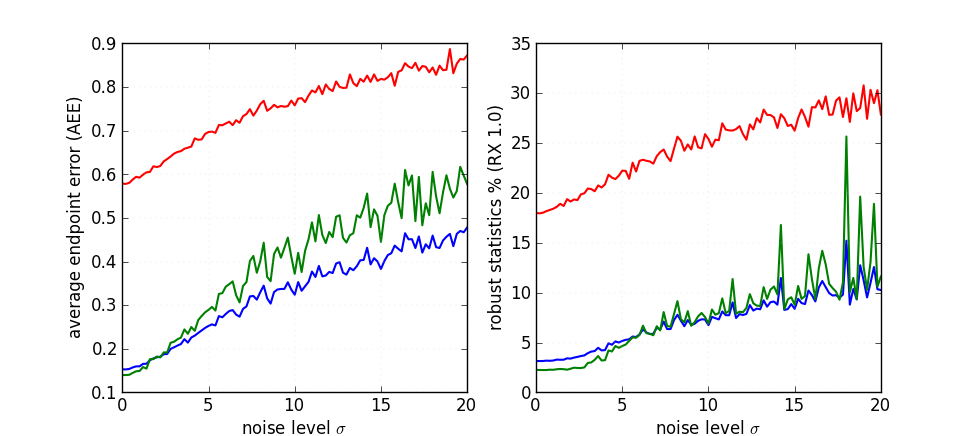
\includegraphics[scale=0.6]{figures/exp_noise_rub.png}}
%  }
%  \caption[Fixed vs Optimal]{\todo{Update image and caption} Comparison between optimized and fixed parameters models on noisy \textit{Dataset 1}  \textbf{Top Left:} First frame of original sequence. \textbf{Top Right:}  Parameter +1. \textbf{Bottom Left:} Parameter +2. \textbf{Bottom Right:} Parameter +3.}
%  \label{fig:noise_fixed_optimal}
%\end{figure*}

%\comment{1. Take baseline algorithm with the best parameters (without optimisations) to show performance drop.
%\textbf{Run:} For each dataset: For all input images (noise): run on fixed parameter set } 
%
%\comment{2. Take baseline algorithm. Parameters: robust, flow-driven, no CLG, no median. Optimize alpha, sigma for each run
%\textbf{Run:} For each dataset: For all input images (noise): run with parameter optimization }


%\change{Another important aspect when showing the results of optical flow computation with or without a ground truth is to present not only the full description of the model used for the computation, but also a  model parameters. However, this is also not enough. If the parameters were optimisazed, a full range of parameters and optimization strategy should also be given.  
%Such situation does not happening in the literature during evaluation of the algorithms, which clearly limits the transparency a of the experimental conditions.}

%\subsection{Optimization of a Single Parameter}
\subsection{Optimization of Individual Parameter}

First we start with the evaluate and discussion of different model parameters of optical flow computation. The aim is to identify the set of paramters which are general and allow to obtain accurate and robust results. Selecting the best paramters we obtain a basis for our \textit{baseline method} which will be presented later in the chapter (See Section \ref{baseline_method}). Moreover, during the evaluation we highlight the importance of such optimization and provide a general guidance to perform it. Here we evaluate the most basis components of optical flow computation, such as derivatives approximation, number of warping levels and warping scale factor.




\subsubsection{Derivatives Approximation}

In Section \ref{discretization} a number of alternatives to represent image derivatives were outlined. Here we  compare different stencil modes and draw the conclusions about their appropriate usage for different image properties. For that, we consider two important aspects from our Data Taxonomy Section \ref{data_taxonomy}, namely the influence of noise and low contrast (low spatial image gradient). To check the performance on noisy data we restrict our study to \textit{Gaussian noise} model \ref{noise_models}, since it introduces sufficient disturbances to the image data.
For the evaluation we fix all the model parameters (which were optimized ahead), and vary only the computation schemes for derivatives approximation. The results for noisy data are shown in Table \ref{tab:derivatives_noise} and for low-contrast data in Table \ref{tab:derivatives_contrast}. 

With respect to noisy data we can make the following observations: 
\begin{itemize}
	\item \textit{Temporal averaging improves the results}. From the evaluation result we conclude that temporal averaging of is useful for both original and noise datasets and provided a robust scheme for derivatives. However, one should be confident that the displacements between corresponding image pairs are small, so such step could be performed. In the presence of large displacements we employ multi-level strategy, discussed in Section \ref{multilevel}. The appropriate choice for the warping scale and number of warping levels we discuss in Section \ref{opt_warping_scale} and Section \ref{opt_warping_levels} respectively. 
	\item \textit{Increased sensitivity of fourth-order derivatives to noise}. Despite the facts, that fourth-order derivatives approximation may lead to a significant improvements in accuracy for the original, noise-free images, it does not perform well on noise data. In the presence of noise a second-order approximation performs better for all noise levels. This might be explained by the increased sensitivity of the fourth order-derivative scheme to noise.
\end{itemize}
    
      
% Table generated by Excel2LaTeX from sheet 'noise'
\begin{table}[ht] \scriptsize
  \centering
  \caption{Comparison between spatial derivatives approximation schemes on noisy \rub dataset. The following computation schemes are compared:  second-order, second-order with temporal averaging, fourth order and fourth-order with temporal averaging. An additive \textit{Gaussian noise} with a zero-mean and standard deviations $\sigma$=0, 5, 10, 20 was introduced.}
    \begin{tabular}{ccccc}
    \toprule
    %\hline
    \multicolumn{1}{c}{noise} & \multicolumn{1}{ c}{model} & \multicolumn{3}{c}{error} \\ 
    \midrule
          &       & \textit{all}    & \textit{disc}   & \textit{untext}  \\ 
    \midrule
     \midrule
    \multicolumn{1}{c}{\multirow{4}[0]{*}{$\sigma$ = 0}} & \multicolumn{1}{l}{2nd order} & 0.172 & 0.683 & 0.135 \\
    \multicolumn{1}{c}{} & \multicolumn{1}{l}{2nd order + temp} & 0.161 & 0.628 & 0.13 \\
    \multicolumn{1}{c}{} & \multicolumn{1}{l}{4th order} & 0.169 & 0.673 & 0.132 \\
    \multicolumn{1}{c}{} & \multicolumn{1}{l}{4th order + temp} & \textbf{0.157} & \textbf{0.605} & \textbf{0.127} \\ 
    \midrule
    \multicolumn{1}{c}{\multirow{4}[0]{*}{$\sigma$ = 5}} & \multicolumn{1}{l}{2nd order} & 0.315 & 0.822 & 0.289 \\
    \multicolumn{1}{c}{} & \multicolumn{1}{l}{2nd order + temp} & \textbf{0.284} & \textbf{0.748} & \textbf{0.264} \\
    \multicolumn{1}{c}{} & \multicolumn{1}{l}{4th order} & 0.343 & 0.841 & 0.311 \\
    \multicolumn{1}{c}{} & \multicolumn{1}{l}{4th order + temp} & 0.304 & 0.751 & 0.273 \\
    \midrule
    \multicolumn{1}{c}{\multirow{4}[0]{*}{$\sigma$ = 10}} & \multicolumn{1}{l}{2nd order} & 0.581 & 1     & 0.544 \\
    \multicolumn{1}{c}{} & \multicolumn{1}{l}{2nd order + temp} & \textbf{0.506} & \textbf{0.921} & \textbf{0.454} \\
    \multicolumn{1}{c}{} & \multicolumn{1}{l}{4th order} & 0.664 & 1.037 & 0.652 \\
    \multicolumn{1}{c}{} & \multicolumn{1}{l}{4th order + temp} & 0.593 & 0.951 & 0.564 \\
    \midrule
    \multicolumn{1}{c}{\multirow{4}[1]{*}{$\sigma$ = 20}} & \multicolumn{1}{l}{2nd order} & 1.414 & 1.584 & 1.508 \\
    \multicolumn{1}{c}{} & \multicolumn{1}{l}{2nd order + temp} & \textbf{1.317} & \textbf{1.502} & \textbf{1.416} \\
    \multicolumn{1}{c}{} & \multicolumn{1}{l}{4th order} & 1.494 & 1.622 & 1.63 \\
    \multicolumn{1}{c}{} & \multicolumn{1}{l}{4th order + temp} & 1.45  & 1.576 & 1.6 \\
    \bottomrule
    \end{tabular}%
  \label{tab:derivatives_noise}%
\end{table}%

We can make the following conclusions about influence of different derivatives approximations on data with low contrast:
\begin{itemize}
	\item \textit{Usefulness of temporal averaging}. The same as for the case of noisy data, temporal averaging show to be effective to improve the accuracy of the optical flow computation. 
	\item \textit{Improved accuracy using fourth-order derivatives}. The accuracy of optical flow computation is improved using fourth-order derivatives approximation.
\end{itemize}

The evaluation of derivatives approximation schemes on \hyd and \mar datasets shows similar outcomes.  
Summarizing both experimental results we may conclude the following: in the presence of substantial noise we choose second-order derivatives with temporal averaging, if noise level is low or can be significantly reduced using preprocessing step we opt to use fourth-order derivatives with temporal averaging. 




% Table generated by Excel2LaTeX from sheet 'contrast'
\begin{table}[ht] \scriptsize
  \centering
  \caption{Comparison between spatial derivatives approximation schemes on  \rub dataset with low contrast. The following computation schemes are compared:  second-order, second-order with temporal averaging, fourth order and fourth-order with temporal averaging. A decrease to a contrast level of $C$=100\%, 50\%, 25\%, 10\% was introduced.}
    \begin{tabular}{ccccc}
    \toprule
    \multicolumn{1}{c}{contrast} & \multicolumn{1}{c}{model} & \multicolumn{3}{c}{error} \\
    \midrule
          &       & \multicolumn{1}{c}{\textit{all}} & \multicolumn{1}{c}{\textit{disc}} & \multicolumn{1}{c}{\textit{untext}} \\
          \midrule
          \midrule
    \multicolumn{1}{c}{\multirow{4}[0]{*}{$C$ = 100\%}} & \multicolumn{1}{l}{2nd order} & 0.172 & 0.683 & 0.135 \\
    \multicolumn{1}{c}{} & \multicolumn{1}{l}{2nd order + temp} & 0.161 & 0.628 & 0.13 \\
    \multicolumn{1}{c}{} & \multicolumn{1}{l}{4th order} & 0.169 & 0.673 & 0.132 \\
    \multicolumn{1}{c}{} & \multicolumn{1}{l}{4th order + temp} & \textbf{0.157} & \textbf{0.605} & \textbf{0.127} \\
     \midrule
    \multicolumn{1}{c}{\multirow{4}[0]{*}{$C$ = 50\%}} & \multicolumn{1}{l}{2nd order} & 0.224 & 0.681 & 0.238 \\
    \multicolumn{1}{c}{} & \multicolumn{1}{l}{2nd order + temp} & 0.214 & 0.667 & 0.223 \\
    \multicolumn{1}{c}{} & \multicolumn{1}{l}{4th order} & 0.207 & 0.662 & 0.213 \\
    \multicolumn{1}{c}{} & \multicolumn{1}{l}{4th order + temp} & \textbf{0.193} & \textbf{0.64} & \textbf{0.195} \\
     \midrule
    \multicolumn{1}{c}{\multirow{4}[0]{*}{$C$ = 25\%}} & \multicolumn{1}{l}{2nd order} & 0.3   & 0.729 & 0.348 \\
    \multicolumn{1}{c}{} & \multicolumn{1}{l}{2nd order + temp} & 0.293 & 0.721 & 0.334 \\
    \multicolumn{1}{c}{} & \multicolumn{1}{l}{4th order} & 0.284 & 0.717 & 0.325 \\
    \multicolumn{1}{c}{} & \multicolumn{1}{l}{4th order + temp} & \textbf{0.275} & \textbf{0.707} & \textbf{0.308} \\
     \midrule
    \multicolumn{1}{c}{\multirow{4}[0]{*}{$C$ = 10\%}} & \multicolumn{1}{l}{2nd order} & 0.41  & 0.797 & 0.48 \\
    \multicolumn{1}{c}{} & \multicolumn{1}{l}{2nd order + temp} & 0.398 & 0.791 & 0.461 \\
    \multicolumn{1}{c}{} & \multicolumn{1}{l}{4th order} & 0.385 & 0.785 & 0.451 \\
    \multicolumn{1}{c}{} & \multicolumn{1}{l}{4th order + temp} & \textbf{0.372} & \textbf{0.776} & \textbf{0.427} \\
    \bottomrule
    \end{tabular}%
  \label{tab:derivatives_contrast}%
\end{table}%




\subsubsection{Warping Levels}
\label{opt_warping_levels}

In order to deal with large displacements  according to our multi-level computation strategy (Section \ref{multilevel}) one has to construct image pyramid. For that purpose a scaling function is used which transfers the original image version to a coarser resolution level and interpolates the obtained results back to the finer computation level. Thus, on each computation level $k$ the image size is determined via:
$$ N^k_{d} = N^{orig} _{d} \eta^k,$$
where $\eta$ is a warping scale parameter, $N_d$ denotes the image size in the dimension $d \in (x,y)$.
In general, to get the best results and capture whole range of displacements (including the fastest motion) one may downscale the image as much as possible. However, for large images with small or moderate displacement values this strategy could result in a substantial loss of performance in terms of computation time. In fact, the aim is to downscale the original image in such a way, that the large displacements become small-scale on the lowest resolution level, so the linearized data constancy assumption can be employed. As soon as it is achieved, further downscaling provide no additional improvement. We illustrate this situation on the \rub dataset in Figure \ref{fig:opt_warping_levels}. Ideally, if the motion model is know or can be deduced from the original image sequence, it is possible to extract the optimal coarsest image size (e.g. number of warping levels) automatically.

\begin{figure*}[ht]
  \centerline{
    \mbox{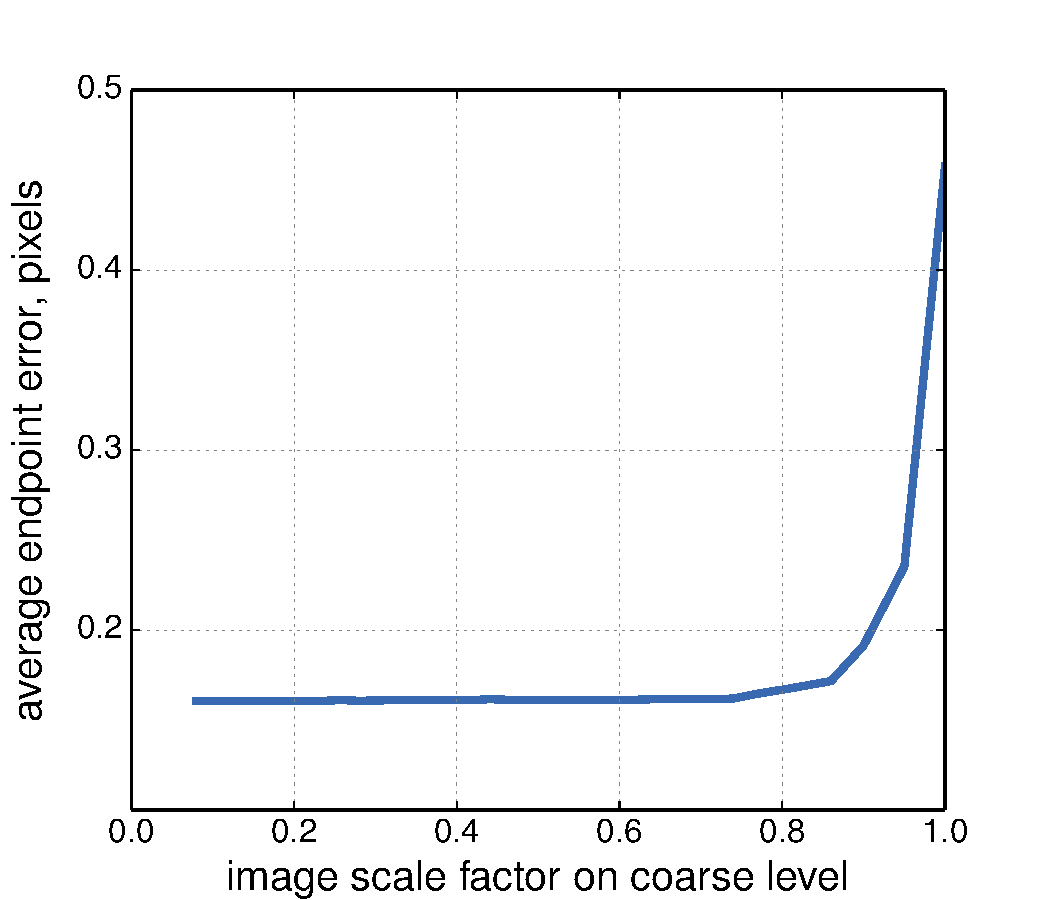
\includegraphics[width=0.45\textwidth]{figures/opt_warping_levels.pdf}}
    \mbox{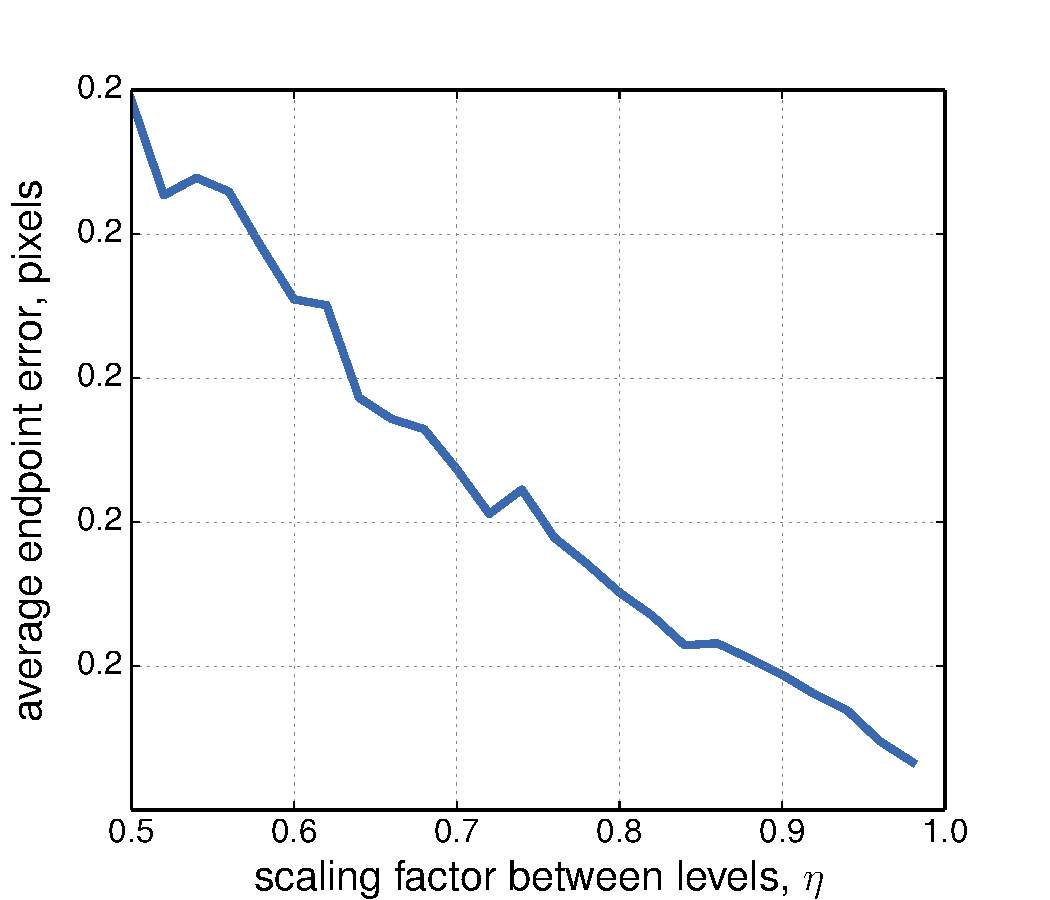
\includegraphics[width=0.45\textwidth]{figures/exp_optimize_scaling_factor.pdf}}
  }  
  \caption{Dependence of optical flow accuracy on a number of levels (coarse scale size) and a scaling factor $\eta$. \textbf{Left:} Improvement of average endpoint error for decreased image size on the coarsest resolution level. All the parameters were fixed as for \textit{baseline} method, warping scale factor $\eta$ = 0.95. Note, that these is no further improvement after a certain scale factor is reached. \textbf{Right:} Improvement of average endpoint error for increasing scaling factor. All the parameters were fixed as for \textit{baseline} method, a number of required warping levels is chosen according to a minimum possible coarsest image size.}
  \label{fig:opt_warping_levels}
\end{figure*}

Here we propose to use two strategies:

\begin{itemize}
	\item \textit{Estimation based on maximum velocity}. We compute the coarsest resolution image size via $ N^k = N^{orig}*S_{max}$, where $S_{max}=\frac{1}{max(\textbf{w})}$ is a scale factor and $max(\textbf{w})$ represents maximum displacement value for the current image pair.
	\item \textit{Estimation based on mean velocity}. We compute in a similar manner as a previous measure, but using mean velocity. Such measure can be reasonable in case if it is known that objects are moving with similar velocities. To account for velocity variations we include the standard deviation value of the velocities distribution. The final measure reads  $ N^k = N^{orig}*S_{mean}$, where $S_{mean}=\frac{1}{mean(\textbf{w}) + std(\textbf{w})}$. 
\end{itemize}

We compare both measures in the Table \ref{tab:opt_derivatives}. How we compute $S_{best}$: we increase the amount of warping levels (decreased image size on the coarsest resolution level) as long as there is a substantial improvement (more then 0.001 for AEE measure and 0.1\% for RX1.0 measure).  

\begin{table}[ht] \scriptsize
\centering
\caption{Comparison of methods to select an appropriate number of warping levels for \textit{RubberWhale}, \hyd and \mar datasets.}
\begin{tabular}{ccccccc}
\toprule
dataset & max   & mean & std & $S_{best}$ & $S_{max}$ & $S_{mean}$   \\ 
\midrule
\midrule
\rub     & 4.616 & 1.236 & 0.505 & 0.7 & 0.22 & \textbf{0.57}  \\ 
\hyd     & 11.12 & 3.48 & 1.452  & 0.57 & 0.09 & \textbf{0.2}  \\ 
\mar     & 2.09  & 1.64 & 0.166  & 0.66 & 0.48 & \textbf{0.55} \\ 
\bottomrule
\end{tabular}
\label{tab:opt_derivatives}%
\end{table}

Conclusions about automated selection of coarsest resolution image size:
\begin{itemize}
	\item \textit{Maximum-based measure provides good results}. This measure provides a reasonable precision and adapts to the image size and correctly handles largest displacements,  but computations on the coarsest levels introduced by the measure can be redundant. This can be seen from the comparison between $S_{best}$ and $S_{max}$ for the \hyd dataset. By default, if we are interested in computing an accurate optical flow we choose this measure.
	\item \textit{Mean-value improves the computation time}. This measure improves the computation time by adapting image to the mean velocity magnitudes and consequently considering less image levels. This measure is closer to the $S_{best}$ scale factor, however could provide poor results for large displacements.    
\end{itemize}
  
 

\subsubsection{Warping Scale}
\label{opt_warping_scale}


In general, the warping scaling factor should be as small as possible to guarantee a smooth transfer between warping levels. However, to small value will result in a very large number of warping levels, hence find compromise. An influence of scaling factors on \rub dataset on the overall precision of optical flow is shown in Figure \ref{fig:opt_warping_levels}.

A range of values between 0.9 and 0.95 is a good compromise between accuracy and running time.

%------------------------
% Does not look useful
%------------------------

%
%\subsubsection{Number of Iterations [SKIP?]}
%
%Three strategies to choose an appropriate number of iteration for the optimization procedure: \ref{iterative_methods}:
%\begin{itemize}
%	\item fixed
%	\item adaptive
%	\item stooping criteria
%\end{itemize}
%
%For Rub - the more the better (dense flow), For Mar - inproves on disc, but gets a bit worse in all regions. \todo{Try on a sequence with homogeneous (smooth) background. Situation could be different}


%---------------------------------------------
%---------------------------------------------
% Include section on multiple paramters
%---------------------------------------------
%---------------------------------------------

\subsection{Optimization of Multiple Parameters}

In this section we generalize the idea of parameters optimization and extend it for multiple parameters.
To highlight the importance of optimization of all model parameters we show several experiments related to three modes of smoothness, namely - data smoothness via presmoothing parameter $\sigma$ (See Section \ref{general_model}), flow smoothness $\alpha$ (See Section \ref{smoothness_assumptions}) and integration scale $\rho$.
First, we optimize one individual parameters, then a pair of smoothness paramters, and finally all the paramters related to smoothness. The quantitative results are presented in Table \ref{tab:exp_smooth3}.  

Analysing the results it is evident that all there smoothness parameters are crucial to provide  accurate and reliable optical flow and should be optimized simultaneously.


%\begin{figure*}[ht]
%  
%  \centerline{
%    \mbox{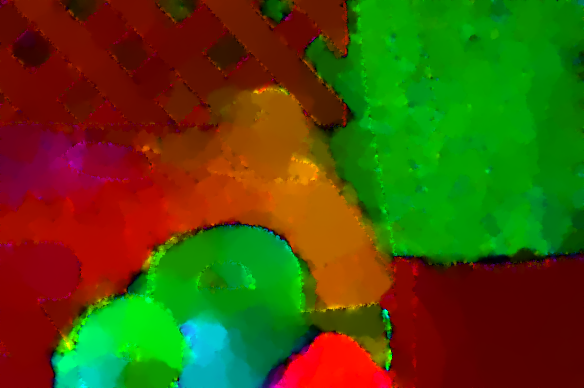
\includegraphics[scale=0.26]{figures/exp_smooth3_a_s.png}}
%    \mbox{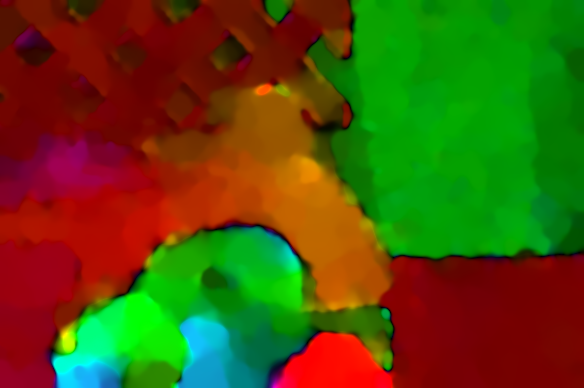
\includegraphics[scale=0.26]{figures/exp_smooth3_a_r.png}}
%    \mbox{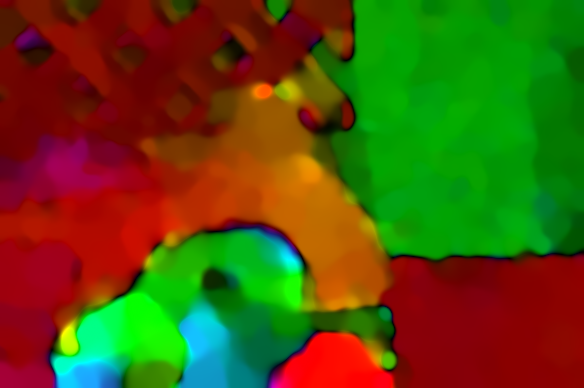
\includegraphics[scale=0.26]{figures/exp_smooth3_s_r.png}}
%  }
%  \vspace{3pt}
%  \centerline{
%    \mbox{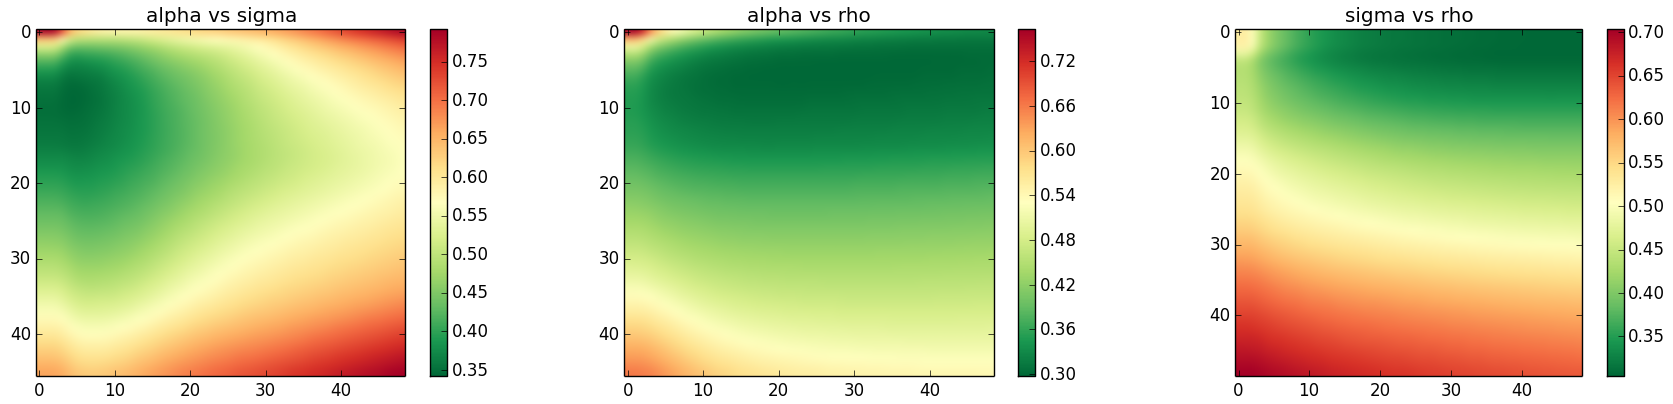
\includegraphics[scale=0.28]{figures/exp_smooth3_flows.png}}
%  }
%  
%  \caption[]{\todo{Change caption} Comparison between three smoothness modes for optical flow computation. \textbf{Left Column:} Optimization of $\alpha$ and $\sigma$ parameters. \textbf{Left Column:} Optimization of $\alpha$ and $\rho$ parameters. \textbf{Left Column:} Optimization of $\sigma$ and $\rho$ parameters. \textbf{Top Row:} The best optical flow result using color coding. \textbf{Bottom Row:} Dependence of corresponding parameters.}
%  \label{fig:exp_smooth3}
%\end{figure*}






\begin{table}[ht] \scriptsize
  \centering
  \caption{Comparison between optimization of a single and simultaneous optimization of several model parameters. As an example we use there kinds of smoothness parameters: data smoothness via presmoothing parameter ($\sigma$), flow smoothness ($\alpha$) and integration scale ($\rho$).}
    \begin{tabular}{rrcrrrrr}
    \toprule
    number & \multicolumn{1}{c}{model} & \multicolumn{3}{c}{error} & \multicolumn{3}{c}{model parameters} \\
    \midrule
              &       & \textit{all} & \multicolumn{1}{c}{\textit{disc}} & \multicolumn{1}{c}{\textit{untext}} & \multicolumn{1}{c}{\textit{alpha}} & \multicolumn{1}{c}{\textit{sigma}} & \multicolumn{1}{c}{\textit{rho}} \\
          \midrule
          \midrule
          
    \multirow{3}[0]{*}{one } & \multicolumn{1}{l}{optimize $\alpha$} & 0.349 & \multicolumn{1}{c}{\textbf{0.773}} & \multicolumn{1}{c}{0.392} & \multicolumn{1}{l}{7.5} & \multicolumn{1}{l}{0.35} & \multicolumn{1}{l}{--} \\
          & \multicolumn{1}{l}{optimize $\sigma$} & 0.437 & \multicolumn{1}{c}{0.876} & \multicolumn{1}{c}{0.362} & \multicolumn{1}{l}{3.5} & \multicolumn{1}{l}{0.6} & \multicolumn{1}{l}{--} \\      
              & \multicolumn{1}{l}{optimize $\rho$} & \textbf{0.305} & \multicolumn{1}{c}{0.833} & \multicolumn{1}{c}{\textbf{0.314}} & \multicolumn{1}{l}{3.5} & \multicolumn{1}{l}{0.35} & \multicolumn{1}{l}{4.6} \\
          
          \midrule
    \multirow{3}[0]{*}{two} & \multicolumn{1}{l}{optimize $\alpha, \sigma$} & 0.342 & \multicolumn{1}{c}{0.773} & \multicolumn{1}{c}{0.351} & \multicolumn{1}{l}{7.0} & \multicolumn{1}{l}{0.5} & \multicolumn{1}{l}{--} \\
    
          & \multicolumn{1}{l}{optimize $\alpha, \rho$} & 0.298 & \multicolumn{1}{c}{\textbf{0.754}} & \multicolumn{1}{c}{0.313} & \multicolumn{1}{l}{5.0} & \multicolumn{1}{l}{0.35} & \multicolumn{1}{l}{2.7} \\
          & \multicolumn{1}{l}{optimize $\sigma, \rho$} & \textbf{0.305} & \multicolumn{1}{c}{0.832} & \multicolumn{1}{c}{\textbf{0.304}} & \multicolumn{1}{l}{3.5} & \multicolumn{1}{l}{0.4} & \multicolumn{1}{l}{4.6} \\
          
          \midrule
          
    three   & \multicolumn{1}{l}{optimize $\alpha, \sigma, \rho$} & \textbf{0.297} & \multicolumn{1}{c}{\textbf{0.757}} & \multicolumn{1}{c}{\textbf{0.299}} & \multicolumn{1}{l}{4.75} & \multicolumn{1}{l}{0.4} & \multicolumn{1}{l}{3.1} \\
    \bottomrule
    \end{tabular}%
  \label{tab:exp_smooth3}%
\end{table}%




\subsection{Confidence-based Optimization}



In the previous two section we have based our parameters optimization procedure on the use of ground truth data, so we were able to compare the computed results with the real ones. For the real life data (tasks) such information is not available. For this purpose a measure based on the confidence can be used. In Section \ref{confidence_measures} a number of possible confidence measures were presented.

Here we demonstrate an example of comparison of metrics to evaluate the correctness of the result using average endpoint error \ref{endpoint_error} and data constancy error \ref{data_constancy_error}. We vary the paramter of the flow regularization $\alpha$ and measure both metrics. The results are presented in Figure \ref{fig:exp_confifance}.
As it can be observed, even without ground truth result it is possible to judge the reliability of the results and choose a sub-optimal parameter based on confidence-based optimization. 

% \begin{figure*}[ht]
% 	\centerline{
% 		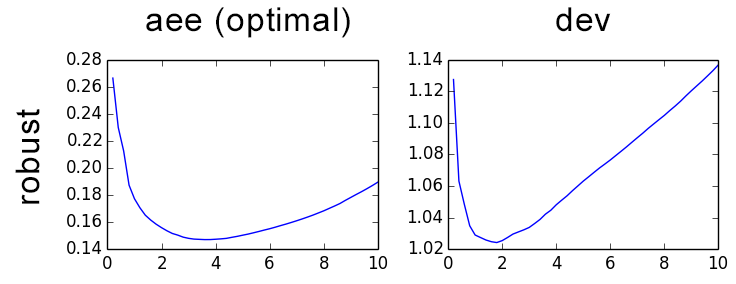
\includegraphics[scale = 0.45]{figures/example_confidance_optimization.png} 
% 	}  
% 	\caption{Comparison between distribution of average endpoint error (AEE) for different values of smoothness parameter $\alpha$ using comparison with a ground truth (optimal) and error metric based on confidence measures.  \textbf{Left:} Average endpoint error given by the comparison of the computed flow field with the ground truth result (\textit{aee}). \textbf{Right:} Data Constancy Error measure (\textit{dev}).}
% 	\label{fig:example_confifance}
% \end{figure*} 

 We further evaluate these measures in the experimental section \ref{exp_confidence_evaluation} and draw conclusions about their appropriate usage. 



\subsection{Baseline Method}
\label{baseline_method}


As it was discussed in the introductory part of the current section, dedicated to parameter optimization, the performance of optical flow largely depends on the set of chosen of model parameters. Since advanced optical flow methods tend to incorporate many features into a single model, it is challenging to separate and evaluate the influence of the individual setting. To provide a basis for a systematic comparison of different settings and model parameters here we describe a \textit{baseline} method which we use in the following experiments section. In all parts where we refer to the baseline method we mean this set of settings.


\begin{table}[ht] \footnotesize
\centering
\caption{A list of all model parameters used for the \textit{baseline} method. If not presented explicitly, all the parameters of the \textit{baseline} method  correspond to the ones given in this table.}
\begin{tabular}{lp{3cm}cp{5cm}}
\toprule
Model parameter & Parameter name & Symbol & Value / Expression   \\ 
\midrule
\midrule
Constancy assumption    & grey value & $D_{grey}(I,\textbf{w})$ & $(\nabla_{3}^{\top}I\textbf{w})^2$ \\ 
Smoothness assumption   & flow-driven & $S_{flow}(u,v)$ & $\Psi_{S}(|\nabla u|^2 + |\nabla v|^2)$, $\Psi_{S}(x) = \sqrt{x + \epsilon}$, $\epsilon = 0.001$ \\ 
Robust function  & Charbonnier penalty & $D_{R}(I,\textbf{w})$ & $ \Psi_R ( (\nabla_{3}^{\top}I\textbf{w})^2)$, $\Psi_{R}(x) = \sqrt{x + \epsilon}$, $\epsilon = 0.001$ \\
Derivatives approximation & second-order and time averaging & $I_x, I_y$ & $\frac{(I_{i+1,j,t+1} - I_{i-1,j,t+1}) + (I_{i+1,j,t} - I_{i-1,j,t})  }{4 h_x}$ \\
Data normalization & -- & $ D_{norm}(I,\textbf{w})$ &  $ \frac{(\nabla_{3}^{\top}I\textbf{w})^2}{|\nabla_2 I(x,y,t)|^2 + \eta} $, disabled \\
Combined local-global & -- & $ D_{CLG}(I,\textbf{w})$ &  $K_{\rho} \ast (\nabla_{3}^{\top}I\textbf{w})^2$ , disabled \\
Median filtering & -- & $  M_p (\textbf{dw}^{k})$ &  $ p \in (3,5)$ , disabled \\
Flow regularization & smoothness parameter & $\alpha$ &  $3.5$ \\
Adaptive regularization & -- & $\alpha(k)$ &  $\alpha$, disabled \\
Presmoothing parameter & standard deviation & $\sigma$ &  $0.35$ \\
Multi-level scheme & warping levels & $k$ &  $15$ \\
Warping accuracy & warping scale & $\eta$ &  $0.9$ \\
\bottomrule
\end{tabular}
\label{tab:baseline}%
\end{table}





 
%--------------------------------------------------------
\section{Quantitative Evaluation}
\label{experiments_synthetic_data}
%--------------------------------------------------------

In this section we present a discussion on the performance, influence of preprocessing, modelling of noise and data outliers and the use of confidence measures. For each experimental evaluation we discuss the advantages and shortcomings of the proposed prototypes. All the results are presented in both a quantitative and a qualitative way. 
For all the experiments we outline important observations and draw the conclusions, which we summarize in the last section of the chapter (See Section \ref{experiments_summary}). In the summary table columns \textit{all}, \textit{disc} and \textit{untext} show the \textit{best possible} result for each region of statistics over the whole range of evaluated parameters.






%--------------------------------------------------------
\subsection{Experiments: Noise}
\label{exp_noise}
%--------------------------------------------------------

\subsubsection{Experiment: Data terms for noisy data}
\label{experiment_data_terms_for_noisy_data}


In this experiment we compare different data terms with respect to their performance on noisy data. To model noise we choose there models - Gaussian, Poisson and Spike noise (see Section \ref{noise_models}), which aim to represent different noise scenarios. While \textit{Gaussian noise} is commonly used in the literature on optical flow to test the robustness of methods in the presence of noise, it is still a simplified noise model. \textit{Poisson noise} is a physically based noise model and correctly describes X-ray data. Finally, \textit{Spike noise} represents a special type of noise with a severe level of image degradation and aims to model data artifacts. Details on the implementation of noise models are given in Section \ref{modeling_image_noise}. We evaluate the performance of data constancy assumptions on noisy data and present our results in Table \ref{tab:noise_data_terms}. For the evaluation we use the \textit{baseline} optical flow method with the optimized  smoothness parameter $\alpha$ and presmoothing parameter $\sigma$. 

% Table generated by Excel2LaTeX from sheet '__all__'
\begin{table}[htbp] \scriptsize
  \centering
  \caption{Performance analysis of data terms on noisy data on the \rub dataset. \textit{Gaussian noise} with zero mean and standard deviation values of $\sigma_n$ = 0, 5, 10, 20 was added. \textit{Poisson noise}: Mean value of the Poisson random distribution $P$ is 0, 50, 200, 400. \textit{Spike Noise}: we randomly replace a certain percentage of pixels with black and the same amount of pixels with white grey value. For the experiment an amount of $S=$0\% (no noise), 2.5\%, 5.0\%, 7.5\% replaced pixels was used. Method: \textit{baseline}, optimized for $\sigma=[0.15 .. 2.5]$, $\alpha=[1.0 .. 40]$.}
    \begin{tabular}{crrrrrrrrrrrr}
    \toprule
    model & \multicolumn{4}{c}{Gaussian noise} & \multicolumn{4}{c}{Poisson noise} & \multicolumn{4}{c}{Spike noise} \\
    \midrule
          & \multicolumn{1}{c}{$\sigma_n$} & \multicolumn{3}{c}{error} & \multicolumn{1}{c}{$P$} & \multicolumn{3}{c}{error} & \multicolumn{1}{c}{$S$} & \multicolumn{3}{c}{error} \\
          
          \midrule
          
          
          & \multicolumn{1}{c}{} & \multicolumn{1}{c}{\textit{all}} & \multicolumn{1}{c}{\textit{disc}} & \multicolumn{1}{c}{\textit{untext}} & \multicolumn{1}{c}{} & \multicolumn{1}{c}{\textit{all}} & \multicolumn{1}{c}{\textit{disc}} & \multicolumn{1}{c}{\textit{untext}} & \multicolumn{1}{c}{} & \multicolumn{1}{c}{\textit{all}} & \multicolumn{1}{c}{\textit{disc}} & \multicolumn{1}{c}{\textit{untext}} \\
          
          \midrule
          \midrule
          
    grey  & \multicolumn{1}{r}{\multirow{4}[1]{*}{0}} & \multicolumn{1}{c}{0.159} & \multicolumn{1}{c}{0.622} & \multicolumn{1}{c}{0.13} & \multicolumn{1}{r}{\multirow{4}[1]{*}{0}} & \multicolumn{1}{c}{0.159} & \multicolumn{1}{c}{0.622} & \multicolumn{1}{c}{0.13} & \multicolumn{1}{r}{\multirow{4}[1]{*}{0 \%}} & \multicolumn{1}{c}{0.159} & \multicolumn{1}{c}{0.622} & \multicolumn{1}{c}{0.13} \\
    grad  &       & \multicolumn{1}{c}{\textbf{0.11}} & \multicolumn{1}{c}{\textbf{0.526}} & \multicolumn{1}{c}{\textbf{0.073}} &       & \multicolumn{1}{c}{\textbf{0.11}} & \multicolumn{1}{c}{\textbf{0.526}} & \multicolumn{1}{c}{\textbf{0.073}} &       & \multicolumn{1}{c}{\textbf{0.11}} & \multicolumn{1}{c}{\textbf{0.526}} & \multicolumn{1}{c}{\textbf{0.073}} \\
    lapl  &       & \multicolumn{1}{c}{0.127} & \multicolumn{1}{c}{0.566} & \multicolumn{1}{c}{0.077} &       & \multicolumn{1}{c}{0.562} & \multicolumn{1}{c}{0.075} & \multicolumn{1}{c}{0.13} &       & \multicolumn{1}{c}{0.562} & \multicolumn{1}{c}{0.075} & \multicolumn{1}{c}{0.13} \\
    norm  &       & \multicolumn{1}{c}{0.137} & \multicolumn{1}{c}{0.607} & \multicolumn{1}{c}{0.095} &       & \multicolumn{1}{c}{0.602} & \multicolumn{1}{c}{0.094} & \multicolumn{1}{c}{0.201} &       & \multicolumn{1}{c}{0.602} & \multicolumn{1}{c}{0.094} & \multicolumn{1}{c}{0.201} \\
    
    \midrule
    
    grey  & \multicolumn{1}{r}{\multirow{4}[2]{*}{5}} & \multicolumn{1}{c}{0.26} & \multicolumn{1}{c}{0.722} & \multicolumn{1}{c}{0.261} & \multicolumn{1}{r}{\multirow{4}[2]{*}{50}} & \multicolumn{1}{c}{0.391} & \multicolumn{1}{c}{\textbf{0.798}} & \multicolumn{1}{c}{0.479} & \multicolumn{1}{r}{\multirow{4}[2]{*}{2.5\%}} & \multicolumn{1}{c}{\textbf{0.437}} & \multicolumn{1}{c}{0.838} & \multicolumn{1}{c}{0.576} \\
    grad  &       & \multicolumn{1}{c}{\textbf{0.233}} & \multicolumn{1}{c}{\textbf{0.689}} & \multicolumn{1}{c}{\textbf{0.242}} &       & \multicolumn{1}{c}{\textbf{0.383}} & \multicolumn{1}{c}{0.799} & \multicolumn{1}{c}{\textbf{0.416}} &       & \multicolumn{1}{c}{0.543} & \multicolumn{1}{c}{0.92} & \multicolumn{1}{c}{0.614} \\
    lapl  &       & \multicolumn{1}{c}{0.273} & \multicolumn{1}{c}{0.712} & \multicolumn{1}{c}{0.303} &       & \multicolumn{1}{c}{0.496} & \multicolumn{1}{c}{0.851} & \multicolumn{1}{c}{0.646} &       & \multicolumn{1}{c}{0.965} & \multicolumn{1}{c}{\textbf{0.74}} & \multicolumn{1}{c}{\textbf{0.099}} \\
    norm  &       & \multicolumn{1}{c}{0.269} & \multicolumn{1}{c}{0.729} & \multicolumn{1}{c}{0.272} &       & \multicolumn{1}{c}{0.395} & \multicolumn{1}{c}{0.809} & \multicolumn{1}{c}{0.464} &       & \multicolumn{1}{c}{0.937} & \multicolumn{1}{c}{0.658} & \multicolumn{1}{c}{0.104} \\
    
    \midrule
    
   
    grey  & \multicolumn{1}{r}{\multirow{4}[2]{*}{10}} & \multicolumn{1}{c}{0.346} & \multicolumn{1}{c}{0.774} & \multicolumn{1}{c}{0.359} & \multicolumn{1}{r}{\multirow{4}[2]{*}{200}} & \multicolumn{1}{c}{0.449} & \multicolumn{1}{c}{\textbf{0.848}} & \multicolumn{1}{c}{0.554} & \multicolumn{1}{r}{\multirow{4}[2]{*}{5.0\%}} & \multicolumn{1}{c}{\textbf{0.611}} & \multicolumn{1}{c}{0.902} & \multicolumn{1}{c}{0.683} \\
    grad  &       & \multicolumn{1}{c}{\textbf{0.331}} & \multicolumn{1}{c}{\textbf{0.767}} & \multicolumn{1}{c}{\textbf{0.346}} &       & \multicolumn{1}{c}{\textbf{0.44}} & \multicolumn{1}{c}{0.852} & \multicolumn{1}{c}{\textbf{0.497}} &       & \multicolumn{1}{c}{0.67} & \multicolumn{1}{c}{0.992} & \multicolumn{1}{c}{0.732} \\
    lapl  &       & \multicolumn{1}{c}{0.411} & \multicolumn{1}{c}{0.802} & \multicolumn{1}{c}{0.48} &       & \multicolumn{1}{c}{0.596} & \multicolumn{1}{c}{0.917} & \multicolumn{1}{c}{0.777} &       & \multicolumn{1}{c}{1.04} & \multicolumn{1}{c}{0.904} & \multicolumn{1}{c}{0.101} \\
    norm  &       & \multicolumn{1}{c}{0.351} & \multicolumn{1}{c}{0.791} & \multicolumn{1}{c}{0.377} &       & \multicolumn{1}{c}{0.467} & \multicolumn{1}{c}{0.873} & \multicolumn{1}{c}{0.556} &       & \multicolumn{1}{c}{1} & \multicolumn{1}{c}{\textbf{0.722}} & \multicolumn{1}{c}{\textbf{0.077}} \\
    
    \midrule
    
    grey  & \multicolumn{1}{r}{\multirow{4}[1]{*}{20}} & \multicolumn{1}{c}{0.474} & \multicolumn{1}{c}{0.866} & \multicolumn{1}{c}{0.567} & \multicolumn{1}{r}{\multirow{4}[1]{*}{400}} & \multicolumn{1}{c}{0.538} & \multicolumn{1}{c}{\textbf{0.897}} & \multicolumn{1}{c}{0.634} & \multicolumn{1}{r}{\multirow{4}[1]{*}{7.5\%}} & \multicolumn{1}{c}{\textbf{0.761}} & \multicolumn{1}{c}{0.978} & \multicolumn{1}{c}{0.733} \\
    grad  &       & \multicolumn{1}{c}{\textbf{0.462}} & \multicolumn{1}{c}{\textbf{0.866}} & \multicolumn{1}{c}{\textbf{0.545}} &       & \multicolumn{1}{c}{\textbf{0.53}} & \multicolumn{1}{c}{0.907} & \multicolumn{1}{c}{\textbf{0.589}} &       & \multicolumn{1}{c}{0.761} & \multicolumn{1}{c}{1.031} & \multicolumn{1}{c}{0.71} \\
    lapl  &       & \multicolumn{1}{c}{0.57} & \multicolumn{1}{c}{0.922} & \multicolumn{1}{c}{0.68} &       & \multicolumn{1}{c}{0.748} & \multicolumn{1}{c}{0.98} & \multicolumn{1}{c}{0.955} &       & \multicolumn{1}{c}{1.083} & \multicolumn{1}{c}{0.847} & \multicolumn{1}{c}{0.098} \\
    norm  &       & \multicolumn{1}{c}{0.471} & \multicolumn{1}{c}{0.882} & \multicolumn{1}{c}{0.566} &       & \multicolumn{1}{c}{0.545} & \multicolumn{1}{c}{0.918} & \multicolumn{1}{c}{0.618} &       & \multicolumn{1}{c}{1.044} & \multicolumn{1}{c}{\textbf{0.713}} & \multicolumn{1}{c}{\textbf{0.06}} \\
    \bottomrule
    \end{tabular}%
  \label{tab:noise_data_terms}%
\end{table}%


From the results of quantitative evaluation we can get the following conclusions:
\begin{itemize}
	\item \textit{Gradient constancy assumption with the robust setting provides good results for both Gaussian and Poisson noise models}. It is reasonable to assume that a derivatives-based constancy assumption will be more sensitive to noise, than a simple grey value assumption. In the work of \cite{BruhnThesis} it was shown that, indeed, the gradient based constancy assumption gives worse performance in comparison with the grey value assumption. However, in the evaluation perform in \cite{BruhnThesis} the robust data term was not used. From our performance analysis it is evident, that the gradient constancy assumption in a robust setting provides better results even for large amounts of noise in all image regions. 
	    
	\item \textit{Higher order derivatives are sensitive to noise for the Gaussian, Poisson and Spike noise models}. Both the Laplacian and Gradient norm constancy assumptions are very sensitive to noise and provide poor results. Thus, these data terms are not useful for X-ray data, which usually contains high amounts of noise. However, one should note, that for noise-free images these data terms outperform the grey value constancy assumption. 
	
	\item \textit{Grey value constancy assumption is more robust for the Spike noise model}. For the Spike noise model the situation is different from the Gaussian noise model. In this case, grey value constancy assumption is more robust to corrupted pixel data. One may notice, that in some cases high order constancy assumptions perform better in \textit{Disc} and \textit{Untext} image regions, however, this situation corresponds to the case when the largest values for smoothing parameters $\alpha$ and $\sigma$ are chosen. In this case the image was oversmoothed, which is seen from the values of \textit{AEE} measure in all image regions. 

	\item \textit{Grey value constancy assumption is more robust for the Spike noise model}. For this noise model the situation is different as for the Gaussian noise model. In this case, the grey value constancy assumption is more robust with respect to corrupted pixel data. One may notice, that in some cases high order constancy assumptions perform better in \textit{Disc} and \textit{Untext} image regions, however, this situation corresponds to the case when the largest values for smoothing parameters $\alpha$ and $\sigma$ are chosen. In this case the image was oversmoothed, which is seen from the values of \textit{AEE} measure in all image regions. 
	
	\item \textit{Grey value constancy assumption is more robust for the Poisson noise model in the regions of image discontinues}.  In general, the Poisson noise model is more challenging then the Gaussian noise model. This is due to the fact that the effect of Gaussian noise can be effectively removed with an appropriate image smoothing. Additionally, the evaluation of results shows that the grey value constancy assumption provides better performance in the regions of image discontinues.  
\end{itemize}





\subsubsection{Experiment: Combined local-global approach}
\label{experimen_combined_local_global_approach}


In this experiment we evaluate the performance of the Combined Local-Global (CLG) approach on noisy data. In the literature on optical flow methods such approaches are not commonly used, especially for synthetic datasets. However, as it was shown in the works of \cite{Bruhn02, Bruhn05a}, such approach can be beneficial in the presence of large amount of noise. We extend the evaluation presented in \cite{BruhnThesis} and perform quantitative evaluation for both the grey value and the gradient value constancy assumptions on \textit{Gaussian} and \textit{Spike} noise models. The evaluation results on the \rub dataset are presented in Table \ref{tab:exp_clg}. The evaluation results are similar for the \hyd and the \mar datasets and excluded from presentation. 





% Table generated by Excel2LaTeX from sheet 'res'
\begin{table}[ht] \scriptsize
  \centering
  \caption{Performance of the Combined Local-Global (CLG) approach on the \textit{Gaussian} and \textit{Spike} noise models on \rub dataset. \textit{Gaussian Noise} with zero mean  and standard deviation values of $\sigma_n$ = 5, 10, 20 was added. For \textit{Spike Noise} an amount $S$  of 2.5\%, 5.0\%, 7.5\% replaced pixels was used. Method: \textit{baseline}, optimized $\rho$ in the range $[0.5 .. 2.0]$, optimized $\sigma$ in the range $[0.35 .. 1.5]$, optimized $\alpha$ in the range $[3.0 .. 40]$.}
    \begin{tabular}{rrrrrrrrr}
    \toprule
          &       & \multicolumn{3}{c}{Gaussian noise} &       & \multicolumn{3}{c}{Spike noise} \\
    \midrule
    \multicolumn{1}{c}{model} & \multicolumn{1}{c}{$\sigma_n$} & \multicolumn{3}{c}{error} & \multicolumn{1}{c}{$S$} & \multicolumn{3}{c}{error} \\
    \midrule
    \multicolumn{1}{c}{} & \multicolumn{1}{c}{\textit{}} & \textit{all} & \multicolumn{1}{c}{\textit{disc}} & \multicolumn{1}{c}{\textit{untext}} & \multicolumn{1}{c}{\textit{}} & \textit{all} & \multicolumn{1}{c}{\textit{disc}} & \multicolumn{1}{c}{\textit{untext}} \\
    \midrule
    \midrule
    \multicolumn{1}{l}{grey} & \multicolumn{1}{c}{\multirow{4}[0]{*}{5}} & 0.26  & \multicolumn{1}{c}{0.722} & \multicolumn{1}{c}{0.261} & \multicolumn{1}{c}{\multirow{4}[0]{*}{2.5\%}} & 0.437 & \multicolumn{1}{c}{0.838} & \multicolumn{1}{c}{0.576} \\
    \multicolumn{1}{l}{grey+CLG} &       & \textbf{0.222} & \multicolumn{1}{c}{\textbf{0.706}} & \multicolumn{1}{c}{\textbf{0.219}} &       & \textbf{0.424} & \multicolumn{1}{c}{0.838} & \multicolumn{1}{c}{0.576} \\
    \multicolumn{1}{l}{grad} &       & 0.233 & \multicolumn{1}{c}{0.689} & \multicolumn{1}{c}{0.242} &       & 0.543 & \multicolumn{1}{c}{0.92} & \multicolumn{1}{c}{0.614} \\
    \multicolumn{1}{l}{grad+CLG} &       & \textbf{0.218} & \multicolumn{1}{c}{0.689} & \multicolumn{1}{c}{\textbf{0.235}} &       & \textbf{0.516} & \multicolumn{1}{c}{\textbf{0.916}} & \multicolumn{1}{c}{\textbf{0.588}} \\
    \midrule
    \multicolumn{1}{l}{grey} & \multicolumn{1}{c}{\multirow{4}[0]{*}{10}} & 0.346 & \multicolumn{1}{c}{0.774} & \multicolumn{1}{c}{0.359} & \multicolumn{1}{c}{\multirow{4}[0]{*}{5.0\%}} & 0.611 & \multicolumn{1}{c}{\textbf{0.902}} & \multicolumn{1}{c}{\textbf{0.683}} \\
    \multicolumn{1}{l}{grey+CLG} &       & \textbf{0.299} & \multicolumn{1}{c}{\textbf{0.755}} & \multicolumn{1}{c}{\textbf{0.3}} &       & \textbf{0.609} & \multicolumn{1}{c}{0.909} & \multicolumn{1}{c}{0.685} \\
    \multicolumn{1}{l}{grad} &       & 0.331 & \multicolumn{1}{c}{\textbf{0.767}} & \multicolumn{1}{c}{0.346} &       & 0.67  & \multicolumn{1}{c}{0.992} & \multicolumn{1}{c}{\textbf{0.732}} \\
    \multicolumn{1}{l}{grad+CLG} &       & \textbf{0.308} & \multicolumn{1}{c}{0.769} & \multicolumn{1}{c}{\textbf{0.328}} &       & \textbf{0.657} & \multicolumn{1}{c}{\textbf{0.981}} & \multicolumn{1}{c}{0.744} \\
    \midrule
    \multicolumn{1}{l}{grey} & \multicolumn{1}{c}{\multirow{4}[0]{*}{20}} & 0.474 & \multicolumn{1}{c}{0.866} & \multicolumn{1}{c}{0.567} & \multicolumn{1}{c}{\multirow{4}[0]{*}{7.5\%}} & 0.761 & \multicolumn{1}{c}{\textbf{0.978}} & \multicolumn{1}{c}{0.733} \\
    \multicolumn{1}{l}{grey+CLG} &       & \textbf{0.434} & \multicolumn{1}{c}{\textbf{0.862}} & \multicolumn{1}{c}{\textbf{0.51}} &       & \textbf{0.711} & \multicolumn{1}{c}{0.985} & \multicolumn{1}{c}{\textbf{0.709}} \\
    \multicolumn{1}{l}{grad} &       & 0.462 & \multicolumn{1}{c}{0.866} & \multicolumn{1}{c}{0.545} &       & 0.761 & \multicolumn{1}{c}{1.031} & \multicolumn{1}{c}{\textbf{0.71}} \\
    \multicolumn{1}{l}{grad+CLG} &       & \textbf{0.443} & \multicolumn{1}{c}{\textbf{0.865}} & \multicolumn{1}{c}{\textbf{0.516}} &       & \textbf{0.739} & \multicolumn{1}{c}{\textbf{1.007}} & \multicolumn{1}{c}{0.714} \\
    \bottomrule

    \end{tabular}%
  \label{tab:exp_clg}%
\end{table}%


Performance evaluation of Combined Local-Global (CLG) approach leads to the following conclusion:
\begin{itemize}
	\item \textit{Integration of local information is useful to improve results on noisy data}. For both constancy assumptions and both noise models used for the evaluation, the Combined Local-Global (CLG) approach gives significantly better results. The performance is better even near the boundaries between moving objects (\textit{disc} region). It can be expected  that in these regions a local integration may spoil the result, but it was not the case. Additionally, the CLG model shows better performance on the \textit{Spike} noise model. As a result of this evaluation,  we make a definite conclusion, that the CLG model is useful for noisy X-ray images.     
\end{itemize}


\subsubsection{Experiment: Normalization of data term}
\label{experiment_normalization_data_term}

In this section we investigate the influence of normalization of data terms. Such approach is relatively novel, but is promising to correct the information in data term, which can be corrupted by noise or image artifacts.  For the evaluation we restrict ourselves to a grey value constancy assumption, however, normalization of other data terms can be performed in a similar manner. Furthermore, we show the performance of data normalization only on \textit{Gaussian noise} model.  The evaluation results on \rub dataset are presented in Table \ref{tab:exp_norm}.

% Table generated by Excel2LaTeX from sheet 'res'
\begin{table}[ht] \scriptsize
  \centering
  \caption{Performance analysis of normalization of data term on noisy data for the \rub dataset. \textit{Gaussian Noise} with zero mean and standard deviation values of $\sigma_n$ = 0 (no noise), 5, 10, 20 was added. For the comparison we use a grey value constancy assumption model \textit{without} data normalization and \textit{without} the CLG approach; a model \textit{with} the CLG; model \textit{with} normalization of the data term; model \textit{with} normalization and the CLG approach.  Method: \textit{baseline}, model = $\lbrace$grey, grey + CLG, grey + norm, grey + norm + CLG$\rbrace$,  optimized $\rho$ in the range $[0.5 .. 2.0]$, optimized  $\eta$ in the range $[0.1 .. 5.0]$, optimized  $\sigma$ in the range $[0.35 .. 1.5]$, optimized  $\alpha$ in the range $[0.5 .. 40]$.}
    \begin{tabular}{crcrr}
    \toprule
    \multicolumn{1}{c}{noise} & \multicolumn{1}{c}{model} & \multicolumn{3}{c}{error} \\
    \midrule
    \multicolumn{1}{c}{} & \multicolumn{1}{c}{} & \textit{all} & \multicolumn{1}{c}{\textit{disc}} & \multicolumn{1}{c}{\textit{untext}} \\
    \midrule
    \midrule
    \multicolumn{1}{r}{\multirow{4}[0]{*}{$\sigma_n$ = 0}} & \multicolumn{1}{l}{grey} & 0.159 & \multicolumn{1}{c}{0.622} & \multicolumn{1}{c}{0.13} \\
          & \multicolumn{1}{l}{grey+CLG} & 0.142 & \multicolumn{1}{c}{0.602} & \multicolumn{1}{c}{\textbf{0.11}} \\
          & \multicolumn{1}{l}{grey+norm} & \textbf{0.14} & \multicolumn{1}{c}{\textbf{0.582}} & \multicolumn{1}{c}{0.111} \\
          & \multicolumn{1}{l}{grey+norm+CLG} & 0.143 & \multicolumn{1}{c}{0.615} & \multicolumn{1}{c}{0.113} \\
          
          \midrule
          
    \multicolumn{1}{r}{\multirow{4}[0]{*}{$\sigma_n$ = 5}} & \multicolumn{1}{l}{grey} & 0.26  & \multicolumn{1}{c}{0.722} & \multicolumn{1}{c}{0.261} \\
          & \multicolumn{1}{l}{grey+CLG} & 0.222 & \multicolumn{1}{c}{0.706} & \multicolumn{1}{c}{0.219} \\
          & \multicolumn{1}{l}{grey+norm} & 0.226 & \multicolumn{1}{c}{\textbf{0.706}} & \multicolumn{1}{c}{0.225} \\
          & \multicolumn{1}{l}{grey+norm+CLG} & \textbf{0.218} & \multicolumn{1}{c}{0.711} & \multicolumn{1}{c}{\textbf{0.215}} \\
          
          \midrule
          
    \multicolumn{1}{r}{\multirow{4}[0]{*}{$\sigma_n$ = 10}} & \multicolumn{1}{l}{grey} & 0.346 & \multicolumn{1}{c}{0.774} & \multicolumn{1}{c}{0.359} \\
          & \multicolumn{1}{l}{grey+CLG} & 0.299 & \multicolumn{1}{c}{\textbf{0.755}} & \multicolumn{1}{c}{0.3} \\
          & \multicolumn{1}{l}{grey+norm} & 0.303 & \multicolumn{1}{c}{0.764} & \multicolumn{1}{c}{0.3} \\
          & \multicolumn{1}{l}{grey+norm+CLG} & \textbf{0.29} & \multicolumn{1}{c}{0.772} & \multicolumn{1}{c}{\textbf{0.29}} \\
          
          \midrule
          
    \multicolumn{1}{r}{\multirow{4}[0]{*}{$\sigma_n$ = 20}} & \multicolumn{1}{l}{grey} & 0.474 & \multicolumn{1}{c}{0.866} & \multicolumn{1}{c}{0.567} \\
          & \multicolumn{1}{l}{grey+CLG} & 0.434 & \multicolumn{1}{c}{0.862} & \multicolumn{1}{c}{\textbf{0.51}} \\
          & \multicolumn{1}{l}{grey+norm} & 0.457 & \multicolumn{1}{c}{\textbf{0.854}} & \multicolumn{1}{c}{0.523} \\
          & \multicolumn{1}{l}{grey+norm+CLG} & \textbf{0.448} & \multicolumn{1}{c}{0.859} & \multicolumn{1}{c}{0.513} \\
    \bottomrule
    \end{tabular}%
  \label{tab:exp_norm}%
\end{table}%

Results of performance evaluation of data term normalization approach are:
\begin{itemize}
	\item \textit{Data normalization improves results on noisy data}. As it was reasoned in Section \ref{normalization}, image locations with high gradient provide more contribution to the overall energy of the data term and thus largely influence the estimation of optical flow. Since such image gradient may be caused by data outliers such as noise or image artifacts, the influence of high image gradient can be intentionally suppressed. From the quantitative evaluation one can see, that the normalization step is indeed helps to improve the results of optical flow.
	    
	\item \textit{Data normalization approach outperforms the Combined Local-Global approach on flow boundaries}. It should be noted, that despite the fact that the CLG model gives better overall performance and improves the result in untextured image regions, the approach based on data normalization gives more accurate results on flow discontinuities. This could be explained by the smoothing properties of local integration in the motion tensor used in the CLG approach.   
	
	\item \textit{Data normalization can be further combined with the CLG approach to improve results}. An important advantage of the data normalization approach, is that it can be further combined with a CLG approach to improve the result of optical flow computation. For all noise levels a combination of both approaches lead to a significant improvement of the result in all image regions.    
\end{itemize}


%--------------------------------------------------------
\subsection{Experiments: Preprocessing}
%--------------------------------------------------------

\subsubsection{Experiment: Noise reduction}
\label{experiment_noise_reduction}


In this section we evaluate the performance of noise reduction techniques and their influence on the accuracy of optical flow methods. An important question to answer in this section is - does an advanced preprocessing procedure improves the results of optical flow? The second important aspect is to reveal the most suitable filtering procedure for the noise scenarios which are used in our evaluation.

We do not attempt to evaluate a large set of possible filtering procedure existing in the literature. Instead, we restrict ourselves to a number of popular filters, which are easy to implement. We evaluate four denoising filters, presented in Section \ref{noise_filters}: 
\begin{itemize}
\item Gaussian smoothing
\item Median filter
\item Bilateral filter
\item Anisotropic diffusion
\end{itemize}
For each individual filter we optimized its parameters and show only the best achievable result in the final evaluation table. Quantitative comparison of denoising filters and influence on the accuracy of flow computation is presented in Table \ref{tab:exp_filter_noise} and Table \ref{tab:exp_filter_noise_gauss_spike} and gives us the following results:   
\begin{itemize}
	\item \textit{Noise filtering of initial data can be helpful.} As it can be observed from the resulting tables, for every noise model and all corresponding noise levels, some kind of preprocessing filter always gave better results.
	    
	\item \textit{For each noise model there is an optimal filtering procedure}. Not surprisingly, a Gaussian smoothing performed significantly better then any other methods on the dataset with \textit{Gaussian} noise. The same situation is true for the median filtering, when it is applied on datasets with \textit{Spike} noise. However, both filtering methods failed to provide good results for datasets, for which they are not well suited. 
	
	\item \textit{Gaussian filtering is a simple and effective filtering procedure}. Despite its simplicity, Gaussian smoothing still provides relatively good results. For \textit{Gaussian} noise model no filter could outperform it, even if all the parameters are carefully optimized.

	\item \textit{Gaussian filtering is useful to remove Poisson noise}. Gaussian filtering shows better performance to remove the \textit{Poisson} noise then the other approaches.  

		\item \textit{Usefulness of Anisotropic diffusion filtering for complex noise scenarios}. It is interesting to note, that anisotropic filter which performed relatively poor on both \textit{Gaussian} and \textit{Spike} noise models, provides the best results in the case when both models are combined (see Table \ref{tab:exp_filter_noise_gauss_spike}). This could be explained by the fact that anisotropic filtering combines smoothing properties of the Gaussian smoothing and ability to filter data outliers as of the median filtering.
				
		\item \textit{The appropriate choice of a filtering procedure and its parameters is crucial, however, a challenging task}.  From the extensive evaluation on multiple datasets and noise models, we conclude that preprocessing of initial (raw) data is useful and allows to achieve more accurate results. However, one should carefully investigate a proper choice of appropriate filtering procedure based on extensive evaluation of the given data.
\end{itemize}


% Table generated by Excel2LaTeX from sheet 'Sheet1'
\begin{table}[ht] \scriptsize
  \centering
  \caption{Performance analysis of noise reduction techniques on \textit{Gaussian}, \textit{Poisson} and \textit{Spike} noise models.  \textit{Gaussian} noise with zero mean  and standard deviation values of $\sigma_n$ = 5, 10, 20, 40 was added. \textit{Poisson} noise: Mean value of Poisson random distribution $P$ = 50, 200, 400, 800. For \textit{Spike} noise an amount $S$ = 2.5\%, 5.0\%, 7.5\%, 10\% replaced pixels was used. Method: \textit{baseline}, filter = $\lbrace \text{no filter}, \text{Gaussian}, \text{Median}, \text{Bilateral}, \text{Anisotropic}  \rbrace$, $\sigma=0.35$, optimized $\alpha$ in the range $[0.5 .. 40]$.}
    \begin{tabular}{rrrrrrrrrrrrr}
    \toprule
          & \multicolumn{4}{c}{Gaussian noise} & \multicolumn{4}{c}{Poisson noise} & \multicolumn{4}{c}{Spike noise} \\
    \midrule
    \multicolumn{1}{c}{filter} & \multicolumn{1}{c}{$\sigma_n$} & \multicolumn{3}{c}{error} & \multicolumn{1}{c}{$P$} & \multicolumn{3}{c}{error} & \multicolumn{1}{c}{$S$} & \multicolumn{3}{c}{error} \\
    
    \midrule
    
          &       & \multicolumn{1}{c}{\textit{all}} & \multicolumn{1}{c}{\textit{disc}} & \multicolumn{1}{c}{\textit{untext}} &       & \multicolumn{1}{c}{\textit{all}} & \multicolumn{1}{c}{\textit{disc}} & \multicolumn{1}{c}{\textit{untext}} &       & \multicolumn{1}{c}{\textit{all}} & \multicolumn{1}{c}{\textit{disc}} & \multicolumn{1}{c}{\textit{untext}} \\
          
          \midrule
          \midrule
          
    \multicolumn{1}{l}{No filter} & \multirow{5}[1]{*}{5} & \multicolumn{1}{c}{0.256} & \multicolumn{1}{c}{0.719} & \multicolumn{1}{c}{0.255} & \multirow{5}[1]{*}{50} & \multicolumn{1}{c}{0.323} & \multicolumn{1}{c}{0.761} & \multicolumn{1}{c}{0.361} & \multirow{5}[1]{*}{2.5\%} & \multicolumn{1}{c}{0.427} & \multicolumn{1}{c}{0.835} & \multicolumn{1}{c}{0.598} \\
    \multicolumn{1}{l}{Gaussian} &       & \multicolumn{1}{c}{\textbf{0.256}} & \multicolumn{1}{c}{\textbf{0.719}} & \multicolumn{1}{c}{\textbf{0.248}} &       & \multicolumn{1}{c}{\textbf{0.319}} & \multicolumn{1}{c}{\textbf{0.761}} & \multicolumn{1}{c}{\textbf{0.348}} &       & \multicolumn{1}{c}{0.408} & \multicolumn{1}{c}{0.83} & \multicolumn{1}{c}{0.554} \\
    \multicolumn{1}{l}{Median} &       & \multicolumn{1}{c}{0.279} & \multicolumn{1}{c}{0.753} & \multicolumn{1}{c}{0.263} &       & \multicolumn{1}{c}{0.339} & \multicolumn{1}{c}{0.791} & \multicolumn{1}{c}{0.367} &       & \multicolumn{1}{c}{\textbf{0.206}} & \multicolumn{1}{c}{\textbf{0.7}} & \multicolumn{1}{c}{\textbf{0.169}} \\
    \multicolumn{1}{l}{Bilateral} &       & \multicolumn{1}{c}{0.26} & \multicolumn{1}{c}{0.73} & \multicolumn{1}{c}{0.25} &       & \multicolumn{1}{c}{0.321} & \multicolumn{1}{c}{0.762} & \multicolumn{1}{c}{0.351} &       & \multicolumn{1}{c}{0.453} & \multicolumn{1}{c}{0.849} & \multicolumn{1}{c}{0.631} \\
    \multicolumn{1}{l}{Anisotropic} &       & \multicolumn{1}{c}{0.388} & \multicolumn{1}{c}{0.819} & \multicolumn{1}{c}{0.396} &       & \multicolumn{1}{c}{0.393} & \multicolumn{1}{c}{0.832} & \multicolumn{1}{c}{0.431} &       & \multicolumn{1}{c}{0.377} & \multicolumn{1}{c}{0.819} & \multicolumn{1}{c}{0.358} \\
    
    \midrule
    
    
    \multicolumn{1}{l}{No filter} & \multirow{5}[2]{*}{10} & \multicolumn{1}{c}{0.349} & \multicolumn{1}{c}{0.773} & \multicolumn{1}{c}{0.392} & \multirow{5}[2]{*}{150} & \multicolumn{1}{c}{0.396} & \multicolumn{1}{c}{0.794} & \multicolumn{1}{c}{0.501} & \multirow{5}[2]{*}{5.0\%} & \multicolumn{1}{c}{0.519} & \multicolumn{1}{c}{0.897} & \multicolumn{1}{c}{0.671} \\
    \multicolumn{1}{l}{Gaussian} &       & \multicolumn{1}{c}{\textbf{0.342}} & \multicolumn{1}{c}{0.773} & \multicolumn{1}{c}{\textbf{0.346}} &       & \multicolumn{1}{c}{\textbf{0.392}} & \multicolumn{1}{c}{\textbf{0.794}} & \multicolumn{1}{c}{0.478} &       & \multicolumn{1}{c}{0.516} & \multicolumn{1}{c}{0.895} & \multicolumn{1}{c}{0.65} \\
    \multicolumn{1}{l}{Median} &       & \multicolumn{1}{c}{0.359} & \multicolumn{1}{c}{0.79} & \multicolumn{1}{c}{0.378} &       & \multicolumn{1}{c}{0.412} & \multicolumn{1}{c}{0.816} & \multicolumn{1}{c}{0.5} &       & \multicolumn{1}{c}{\textbf{0.23}} & \multicolumn{1}{c}{\textbf{0.736}} & \multicolumn{1}{c}{\textbf{0.19}} \\
    \multicolumn{1}{l}{Bilateral} &       & \multicolumn{1}{c}{0.346} & \multicolumn{1}{c}{\textbf{0.772}} & \multicolumn{1}{c}{0.354} &       & \multicolumn{1}{c}{0.396} & \multicolumn{1}{c}{0.794} & \multicolumn{1}{c}{\textbf{0.466}} &       & \multicolumn{1}{c}{0.542} & \multicolumn{1}{c}{0.908} & \multicolumn{1}{c}{0.692} \\
    \multicolumn{1}{l}{Anisotropic} &       & \multicolumn{1}{c}{0.407} & \multicolumn{1}{c}{0.817} & \multicolumn{1}{c}{0.43} &       & \multicolumn{1}{c}{0.45} & \multicolumn{1}{c}{0.834} & \multicolumn{1}{c}{0.538} &       & \multicolumn{1}{c}{0.463} & \multicolumn{1}{c}{0.867} & \multicolumn{1}{c}{0.603} \\
    
    \midrule
    
    
    \multicolumn{1}{l}{No filter} & \multirow{5}[2]{*}{20} & \multicolumn{1}{c}{0.489} & \multicolumn{1}{c}{0.865} & \multicolumn{1}{c}{0.599} & \multirow{5}[2]{*}{400} & \multicolumn{1}{c}{0.468} & \multicolumn{1}{c}{0.841} & \multicolumn{1}{c}{0.576} & \multirow{5}[2]{*}{7.5\%} & \multicolumn{1}{c}{0.666} & \multicolumn{1}{c}{0.977} & \multicolumn{1}{c}{0.73} \\
    \multicolumn{1}{l}{Gaussian} &       & \multicolumn{1}{c}{\textbf{0.471}} & \multicolumn{1}{c}{\textbf{0.857}} & \multicolumn{1}{c}{\textbf{0.563}} &       & \multicolumn{1}{c}{\textbf{0.448}} & \multicolumn{1}{c}{\textbf{0.835}} & \multicolumn{1}{c}{0.553} &       & \multicolumn{1}{c}{0.666} & \multicolumn{1}{c}{0.976} & \multicolumn{1}{c}{0.715} \\
    \multicolumn{1}{l}{Median} &       & \multicolumn{1}{c}{0.495} & \multicolumn{1}{c}{0.867} & \multicolumn{1}{c}{0.573} &       & \multicolumn{1}{c}{0.474} & \multicolumn{1}{c}{0.848} & \multicolumn{1}{c}{0.591} &       & \multicolumn{1}{c}{\textbf{0.263}} & \multicolumn{1}{c}{\textbf{0.769}} & \multicolumn{1}{c}{\textbf{0.214}} \\
    \multicolumn{1}{l}{Bilateral} &       & \multicolumn{1}{c}{0.483} & \multicolumn{1}{c}{0.863} & \multicolumn{1}{c}{0.579} &       & \multicolumn{1}{c}{0.45} & \multicolumn{1}{c}{0.835} & \multicolumn{1}{c}{\textbf{0.552}} &       & \multicolumn{1}{c}{0.692} & \multicolumn{1}{c}{0.988} & \multicolumn{1}{c}{0.746} \\
    \multicolumn{1}{l}{Anisotropic} &       & \multicolumn{1}{c}{0.504} & \multicolumn{1}{c}{0.874} & \multicolumn{1}{c}{0.583} &       & \multicolumn{1}{c}{0.486} & \multicolumn{1}{c}{0.849} & \multicolumn{1}{c}{0.599} &       & \multicolumn{1}{c}{0.534} & \multicolumn{1}{c}{0.91} & \multicolumn{1}{c}{0.65} \\
    
    \midrule
    
    
    \multicolumn{1}{l}{No filter} & \multirow{5}[1]{*}{40} & \multicolumn{1}{c}{0.723} & \multicolumn{1}{c}{0.97} & \multicolumn{1}{c}{0.746} & \multirow{5}[1]{*}{800} & \multicolumn{1}{c}{0.563} & \multicolumn{1}{c}{0.9} & \multicolumn{1}{c}{0.659} & \multirow{5}[1]{*}{10\%} & \multicolumn{1}{c}{0.836} & \multicolumn{1}{c}{1.096} & \multicolumn{1}{c}{0.812} \\
    \multicolumn{1}{l}{Gaussian} &       & \multicolumn{1}{c}{\textbf{0.625}} & \multicolumn{1}{c}{0.937} & \multicolumn{1}{c}{0.648} &       & \multicolumn{1}{c}{\textbf{0.537}} & \multicolumn{1}{c}{0.889} & \multicolumn{1}{c}{0.63} &       & \multicolumn{1}{c}{0.834} & \multicolumn{1}{c}{1.093} & \multicolumn{1}{c}{0.771} \\
    \multicolumn{1}{l}{Median} &       & \multicolumn{1}{c}{0.638} & \multicolumn{1}{c}{0.929} & \multicolumn{1}{c}{\textbf{0.644}} &       & \multicolumn{1}{c}{0.554} & \multicolumn{1}{c}{0.904} & \multicolumn{1}{c}{\textbf{0.622}} &       & \multicolumn{1}{c}{\textbf{0.375}} & \multicolumn{1}{c}{\textbf{0.804}} & \multicolumn{1}{c}{\textbf{0.247}} \\
    \multicolumn{1}{l}{Bilateral} &       & \multicolumn{1}{c}{0.639} & \multicolumn{1}{c}{0.931} & \multicolumn{1}{c}{0.697} &       & \multicolumn{1}{c}{0.542} & \multicolumn{1}{c}{0.891} & \multicolumn{1}{c}{0.63} &       & \multicolumn{1}{c}{0.85} & \multicolumn{1}{c}{1.109} & \multicolumn{1}{c}{0.754} \\
    \multicolumn{1}{l}{Anisotropic} &       & \multicolumn{1}{c}{0.631} & \multicolumn{1}{c}{\textbf{0.928}} & \multicolumn{1}{c}{0.647} &       & \multicolumn{1}{c}{0.556} & \multicolumn{1}{c}{\textbf{0.882}} & \multicolumn{1}{c}{0.659} &       & \multicolumn{1}{c}{0.604} & \multicolumn{1}{c}{0.955} & \multicolumn{1}{c}{0.73} \\
    \bottomrule
    \end{tabular}%
  \label{tab:exp_filter_noise}%
\end{table}%





%% Table generated by Excel2LaTeX from sheet 'Sheet1'
%\begin{table}[ht] \footnotesize
%  \centering
%  \caption{Performance analysis of noise reduction techniques on Gaussian and Poisson noise. Method: \textit{baseline}, $\sigma=0.35$ optimized for $\alpha=[0.5 .. 40]$.}
%    \begin{tabular}{rrcrr}
%    \toprule
%    \multicolumn{1}{c}{noise} & \multicolumn{1}{c}{filter} & \multicolumn{3}{c}{error} \\
%    \midrule
%          &       & \textit{all} & \multicolumn{1}{c}{\textit{disc}} & \multicolumn{1}{c}{\textit{untext}} \\
%          \midrule
%    \multirow{5}[0]{*}{$\sigma$ =5} & \multicolumn{1}{l}{No filter} & 0.256 & \multicolumn{1}{c}{0.719} & \multicolumn{1}{c}{0.255} \\
%          & \multicolumn{1}{l}{Gaussian} & \textbf{0.256} & \multicolumn{1}{c}{\textbf{0.719}} & \multicolumn{1}{c}{\textbf{0.248}} \\
%          & \multicolumn{1}{l}{Median} & 0.279 & \multicolumn{1}{c}{0.753} & \multicolumn{1}{c}{0.263} \\
%          & \multicolumn{1}{l}{Bilateral} & 0.26  & \multicolumn{1}{c}{0.73} & \multicolumn{1}{c}{0.25} \\
%          & \multicolumn{1}{l}{Anisotropic} & 0.388 & \multicolumn{1}{c}{0.819} & \multicolumn{1}{c}{0.396} \\
%          \midrule
%    \multirow{5}[0]{*}{$\sigma$ =10} & \multicolumn{1}{l}{No filter} & 0.349 & \multicolumn{1}{c}{0.773} & \multicolumn{1}{c}{0.392} \\
%          & \multicolumn{1}{l}{Gaussian} & \textbf{0.342} & \multicolumn{1}{c}{0.773} & \multicolumn{1}{c}{\textbf{0.346}} \\
%          & \multicolumn{1}{l}{Median} & 0.359 & \multicolumn{1}{c}{0.79} & \multicolumn{1}{c}{0.378} \\
%          & \multicolumn{1}{l}{Bilateral} & 0.346 & \multicolumn{1}{c}{\textbf{0.772}} & \multicolumn{1}{c}{0.354} \\
%          & \multicolumn{1}{l}{Anisotropic} & 0.407 & \multicolumn{1}{c}{0.817} & \multicolumn{1}{c}{0.43} \\
%          \midrule
%    \multirow{5}[0]{*}{$\sigma$ =20} & \multicolumn{1}{l}{No filter} & 0.489 & \multicolumn{1}{c}{0.865} & \multicolumn{1}{c}{0.599} \\
%          & \multicolumn{1}{l}{Gaussian} & \textbf{0.471} & \multicolumn{1}{c}{\textbf{0.857}} & \multicolumn{1}{c}{\textbf{0.563}} \\
%          & \multicolumn{1}{l}{Median} & 0.495 & \multicolumn{1}{c}{0.867} & \multicolumn{1}{c}{0.573} \\
%          & \multicolumn{1}{l}{Bilateral} & 0.483 & \multicolumn{1}{c}{0.863} & \multicolumn{1}{c}{0.579} \\
%          & \multicolumn{1}{l}{Anisotropic} & 0.504 & \multicolumn{1}{c}{0.874} & \multicolumn{1}{c}{0.583} \\
%          \midrule
%    \multirow{5}[0]{*}{$\sigma$ =40} & \multicolumn{1}{l}{No filter} & 0.723 & \multicolumn{1}{c}{0.97} & \multicolumn{1}{c}{0.746} \\
%          & \multicolumn{1}{l}{Gaussian} & \textbf{0.625} & \multicolumn{1}{c}{0.937} & \multicolumn{1}{c}{0.648} \\
%          & \multicolumn{1}{l}{Median} & 0.638 & \multicolumn{1}{c}{0.929} & \multicolumn{1}{c}{\textbf{0.644}} \\
%          & \multicolumn{1}{l}{Bilateral} & 0.639 & \multicolumn{1}{c}{0.931} & \multicolumn{1}{c}{0.697} \\
%          & \multicolumn{1}{l}{Anisotropic} & 0.631 & \multicolumn{1}{c}{\textbf{0.928}} & \multicolumn{1}{c}{0.647} \\
%    \bottomrule
%    \end{tabular}%
%  \label{tab:exp_filter_noise_gauss}%
%\end{table}%


%% Table generated by Excel2LaTeX from sheet 'Sheet1'
%\begin{table}[ht] \footnotesize
%  \centering
%  \caption{Performance analysis of noise reduction techniques. Poisson noise. Method: \textit{baseline}, $\sigma=0.35$ optimized for $\alpha=[0.5 .. 40]$.}
%    \begin{tabular}{rrcrr}
%    \toprule
%    \multicolumn{1}{c}{noise} & \multicolumn{1}{c}{model} & \multicolumn{3}{c}{error} \\
%    \midrule
%          &       & \textit{all} & \multicolumn{1}{c}{\textit{disc}} & \multicolumn{1}{c}{\textit{untext}} \\
%          \midrule
%    \multirow{5}[1]{*}{P=50} & No filter & 0.323 & \multicolumn{1}{c}{0.761} & \multicolumn{1}{c}{0.361} \\
%          & Gaussian & \textbf{0.319} & \multicolumn{1}{c}{\textbf{0.761}} & \multicolumn{1}{c}{\textbf{0.348}} \\
%          & Median & 0.339 & \multicolumn{1}{c}{0.791} & \multicolumn{1}{c}{0.367} \\
%          & Bilateral & 0.321 & \multicolumn{1}{c}{0.762} & \multicolumn{1}{c}{0.351} \\
%          & Anisotropic & 0.393 & \multicolumn{1}{c}{0.832} & \multicolumn{1}{c}{0.431} \\
%          \midrule
%    \multirow{5}[2]{*}{P=150} & No filter & 0.396 & \multicolumn{1}{c}{0.794} & \multicolumn{1}{c}{0.501} \\
%          & Gaussian & \textbf{0.392} & \multicolumn{1}{c}{\textbf{0.794}} & \multicolumn{1}{c}{0.478} \\
%          & Median & 0.412 & \multicolumn{1}{c}{0.816} & \multicolumn{1}{c}{0.5} \\
%          & Bilateral & 0.396 & \multicolumn{1}{c}{0.794} & \multicolumn{1}{c}{\textbf{0.466}} \\
%          & Anisotropic & 0.45  & \multicolumn{1}{c}{0.834} & \multicolumn{1}{c}{0.538} \\
%          \midrule
%    \multirow{5}[2]{*}{P=400} & No filter & 0.468 & \multicolumn{1}{c}{0.841} & \multicolumn{1}{c}{0.576} \\
%          & Gaussian & \textbf{0.448} & \multicolumn{1}{c}{\textbf{0.835}} & \multicolumn{1}{c}{0.553} \\
%          & Median & 0.474 & \multicolumn{1}{c}{0.848} & \multicolumn{1}{c}{0.591} \\
%          & Bilateral & 0.45  & \multicolumn{1}{c}{0.835} & \multicolumn{1}{c}{\textbf{0.552}} \\
%          & Anisotropic & 0.486 & \multicolumn{1}{c}{0.849} & \multicolumn{1}{c}{0.599} \\
%          \midrule
%    \multirow{5}[1]{*}{P=800} & No filter & 0.563 & \multicolumn{1}{c}{0.9} & \multicolumn{1}{c}{0.659} \\
%          & Gaussian & \textbf{0.537} & \multicolumn{1}{c}{0.889} & \multicolumn{1}{c}{0.63} \\
%          & Median & 0.554 & \multicolumn{1}{c}{0.904} & \multicolumn{1}{c}{\textbf{0.622}} \\
%          & Bilateral & 0.542 & \multicolumn{1}{c}{0.891} & \multicolumn{1}{c}{0.63} \\
%          & Anisotropic & 0.556 & \multicolumn{1}{c}{\textbf{0.882}} & \multicolumn{1}{c}{0.659} \\
%    \bottomrule
%    \end{tabular}%
%  \label{tab:addlabel}%
%\end{table}%



%% Table generated by Excel2LaTeX from sheet 'Sheet1'
%\begin{table}[ht] \footnotesize
%  \centering
%  \caption{Performance analysis of noise reduction techniques. Spike noise. Method: \textit{baseline}, $\sigma=0.35$ optimized for $\alpha=[0.5 .. 40]$.}
%    \begin{tabular}{rrrrr}
%    \toprule
%    \multicolumn{1}{c}{noise} & \multicolumn{1}{c}{filter} & \multicolumn{3}{c}{error} \\
%    \midrule
%          &       & \multicolumn{1}{c}{\textit{all}} & \multicolumn{1}{c}{\textit{disc}} & \multicolumn{1}{c}{\textit{untext}} \\
%          \midrule
%    \multirow{5}[1]{*}{$S_1$} & \multicolumn{1}{l}{No filter} & 0.427 & 0.835 & 0.598 \\
%          & \multicolumn{1}{l}{Gaussian} & 0.408 & 0.83  & 0.554 \\
%          & \multicolumn{1}{l}{Median} & \textbf{0.206} & \textbf{0.7} & \textbf{0.169} \\
%          & \multicolumn{1}{l}{Bilateral} & 0.453 & 0.849 & 0.631 \\
%          & \multicolumn{1}{l}{Anisotropic} & 0.377 & 0.819 & 0.358 \\
%          \midrule
%    \multirow{5}[2]{*}{$S_2$} & \multicolumn{1}{l}{No filter} & 0.519 & 0.897 & 0.671 \\
%          & \multicolumn{1}{l}{Gaussian} & 0.516 & 0.895 & 0.65 \\
%          & \multicolumn{1}{l}{Median} & \textbf{0.23} & \textbf{0.736} & \textbf{0.19} \\
%          & \multicolumn{1}{l}{Bilateral} & 0.542 & 0.908 & 0.692 \\
%          & \multicolumn{1}{l}{Anisotropic} & 0.463 & 0.867 & 0.603 \\
%          \midrule
%    \multirow{5}[1]{*}{$S_3$} & \multicolumn{1}{l}{No filter} & 0.666 & 0.977 & 0.73 \\
%          & \multicolumn{1}{l}{Gaussian} & 0.666 & 0.976 & 0.715 \\
%          & \multicolumn{1}{l}{Median} & \textbf{0.263} & \textbf{0.769} & \textbf{0.214} \\
%          & \multicolumn{1}{l}{Bilateral} & 0.692 & 0.988 & 0.746 \\
%          & \multicolumn{1}{l}{Anisotropic} & 0.534 & 0.91  & 0.65 \\
%    \bottomrule
%    \end{tabular}%
%  \label{tab:exp_filter_noise_spike}%
%\end{table}%


% Table generated by Excel2LaTeX from sheet 'Sheet1'
\begin{table}[ht] \scriptsize
  \centering
  \caption{Performance analysis of noise reduction techniques for complex noise scenarios (combination of the \textit{Gaussian} and \textit{Spike} noise models).  For  \textit{Gaussian Noise} with zero mean and standard deviation values of $\sigma_n$ = 5, 10, 20, 40 was added. For \textit{Spike Noise} an amount $S$ = 2.5\% replaced pixels was used. Method: \textit{baseline}, filter = $\lbrace \text{no filter}, \text{Gaussian}, \text{Median}, \text{Bilateral}, \text{Anisotropic}  \rbrace$, $\sigma=0.35$, optimized $\alpha$ in the range $[0.5 .. 40]$.}
    \begin{tabular}{rrcrr}
    \toprule
    \multicolumn{1}{c}{noise} & \multicolumn{1}{c}{filter} & \multicolumn{3}{c}{error} \\
    \midrule
          &       & \textit{all} & \multicolumn{1}{c}{\textit{disc}} & \multicolumn{1}{c}{\textit{untext}} \\
          \midrule
          \midrule
    \multirow{5}[1]{*}{($\sigma$=5) + $S_1$} & \multicolumn{1}{l}{No filter} & 0.468 & \multicolumn{1}{c}{0.84} & \multicolumn{1}{c}{0.618} \\
          & \multicolumn{1}{l}{Gaussian} & 0.459 & \multicolumn{1}{c}{0.839} & \multicolumn{1}{c}{0.579} \\
          & \multicolumn{1}{l}{Median} & \textbf{0.299} & \multicolumn{1}{c}{\textbf{0.774}} & \multicolumn{1}{c}{\textbf{0.274}} \\
          & \multicolumn{1}{l}{Bilateral} & 0.475 & \multicolumn{1}{c}{0.845} & \multicolumn{1}{c}{0.623} \\
          & \multicolumn{1}{l}{Anisotropic} & 0.412 & \multicolumn{1}{c}{0.815} & \multicolumn{1}{c}{0.435} \\
          \midrule
    \multirow{5}[2]{*}{($\sigma$=10) + $S_1$} & \multicolumn{1}{l}{No filter} & 0.508 & \multicolumn{1}{c}{0.866} & \multicolumn{1}{c}{0.619} \\
          & \multicolumn{1}{l}{Gaussian} & 0.493 & \multicolumn{1}{c}{0.863} & \multicolumn{1}{c}{0.579} \\
          & \multicolumn{1}{l}{Median} & \textbf{0.384} & \multicolumn{1}{c}{\textbf{0.801}} & \multicolumn{1}{c}{\textbf{0.43}} \\
          & \multicolumn{1}{l}{Bilateral} & 0.51  & \multicolumn{1}{c}{0.868} & \multicolumn{1}{c}{0.62} \\
          & \multicolumn{1}{l}{Anisotropic} & 0.445 & \multicolumn{1}{c}{0.837} & \multicolumn{1}{c}{0.525} \\
          \midrule
    \multirow{5}[2]{*}{($\sigma$=20) + $S_1$} & \multicolumn{1}{l}{No filter} & 0.602 & \multicolumn{1}{c}{0.935} & \multicolumn{1}{c}{0.697} \\
          & \multicolumn{1}{l}{Gaussian} & 0.579 & \multicolumn{1}{c}{0.928} & \multicolumn{1}{c}{0.665} \\
          & \multicolumn{1}{l}{Median} & 0.544 & \multicolumn{1}{c}{0.902} & \multicolumn{1}{c}{0.63} \\
          & \multicolumn{1}{l}{Bilateral} & 0.6   & \multicolumn{1}{c}{0.934} & \multicolumn{1}{c}{0.694} \\
          & \multicolumn{1}{l}{Anisotropic} & \textbf{0.51} & \multicolumn{1}{c}{\textbf{0.885}} & \multicolumn{1}{c}{\textbf{0.6}} \\
          \midrule
    \multirow{5}[1]{*}{($\sigma$=40) + $S_1$} & \multicolumn{1}{l}{No filter} & 0.799 & \multicolumn{1}{c}{1.007} & \multicolumn{1}{c}{0.775} \\
          & \multicolumn{1}{l}{Gaussian} & 0.7   & \multicolumn{1}{c}{0.965} & \multicolumn{1}{c}{0.664} \\
          & \multicolumn{1}{l}{Median} & 0.687 & \multicolumn{1}{c}{0.953} & \multicolumn{1}{c}{0.656} \\
          & \multicolumn{1}{l}{Bilateral} & 0.741 & \multicolumn{1}{c}{0.972} & \multicolumn{1}{c}{0.733} \\
          & \multicolumn{1}{l}{Anisotropic} & \textbf{0.651} & \multicolumn{1}{c}{\textbf{0.935}} & \multicolumn{1}{c}{\textbf{0.647}} \\
    \bottomrule
    \end{tabular}%
  \label{tab:exp_filter_noise_gauss_spike}%
\end{table}%





\subsubsection{Experiment: Non-uniform brightness correction}
\label{experiment_nonuniform_brightness}

As the next step, we test the possibility to correct non-uniform brightness, which is a crucial image degradation process affecting computation of optical flow. For this purpose we compare performance of the grey value data term without preprocessing and the same data term, but with prior non-uniform brightness correction. For the evaluation we use the following brightness changes scenarios, described in Section \ref{modeling_brigntenss}:

\begin{itemize}

\item Additive brightness change: for this case a constant value of 30 is added to every pixel of the second image of an input sequence.

\item Multiplicative brightness change: every pixel of the second image frame is multiplied by a factor of 1.5. 

\item Pattern \textit{"Spot"}: this pattern simulates a spatial variation of beam intensity and is implemented as an addition of the initial image with a spatially varying brightness pattern (See Figure \ref{fig:patterns}).

\item Pattern \textit{"Stripes"}: this pattern aims to model brightness variation due to spatial fluctuations of a light source and changing beam intensity. Different strip patterns are added to the first and the second frame of the input sequence (See Figure \ref{fig:patterns}).
\end{itemize}
For the preprocessing procedure we use the image leveling approach using the Gaussian filter (see Section \ref{image_leveling}) with an optimized size of the spatial mask. 

Comparison between a model with and without preprocessing of initial image sequence is shown in Table \ref{tab:exp_filter_bright}.


% Table generated by Excel2LaTeX from sheet 'Sheet4'
\begin{table}[ht] \scriptsize
  \centering
  \caption{Performance of non-uniform brightness correction on the \rub dataset. Four brightness patterns are used for the evaluation: additive, multiplicative, pattern \textit{"Spot"} and pattern \textit{"Stripes"}. Method: \textit{baseline}, model = $\lbrace \text{no filter}, \text{Gaussian leveling} \rbrace$, optimized $\sigma$ in the range $[0.15 .. 1.5]$, optimized $\alpha$ in the range $[0.15 .. 40]$.   }
    \begin{tabular}{cccrr}
    \toprule
    \multicolumn{1}{c}{brightness} & model & \multicolumn{3}{c}{error} \\
    \midrule
          & \textit{} & \textit{all} & \multicolumn{1}{c}{\textit{disc}} & \multicolumn{1}{c}{\textit{untext}} \\
          \midrule
          \midrule
    \multicolumn{1}{l}{\multirow{2}[0]{*}{additive}} & \multicolumn{1}{l}{grey}  & 1.179 & \multicolumn{1}{c}{1.234} & \multicolumn{1}{c}{1.137} \\
          & filter + grey & \textbf{0.128} & \multicolumn{1}{c}{\textbf{0.581}} & \multicolumn{1}{c}{\textbf{0.089}} \\
          
          \midrule
          
    \multicolumn{1}{l}{\multirow{2}[0]{*}{multiplicative}} & \multicolumn{1}{l}{grey}  & 2.125 & \multicolumn{1}{c}{2.003} & \multicolumn{1}{c}{2.901} \\
          & filter + grey & \textbf{0.162} & \multicolumn{1}{c}{\textbf{0.613}} & \multicolumn{1}{c}{\textbf{0.103}} \\
          
          \midrule
          
    \multicolumn{1}{l}{\multirow{2}[0]{*}{\textit{"Spot"}}} & \multicolumn{1}{l}{grey}  & 1.839 & \multicolumn{1}{c}{2.246} & \multicolumn{1}{c}{1.699} \\
          & filter + grey & \textbf{0.128} & \multicolumn{1}{c}{\textbf{0.581}} & \multicolumn{1}{c}{\textbf{0.088}} \\
          
          \midrule
          
    \multicolumn{1}{l}{\multirow{2}[0]{*}{\textit{"Stripes"}}} & \multicolumn{1}{l}{grey}  & 1.062 & \multicolumn{1}{c}{1.318} & \multicolumn{1}{c}{0.816} \\
          & filter + grey & \textbf{0.132} & \multicolumn{1}{c}{\textbf{0.584}} & \multicolumn{1}{c}{\textbf{0.093}} \\
    \bottomrule
    \end{tabular}%
  \label{tab:exp_filter_bright}%
\end{table}%

From the evaluation of quantitative results we can make the following conclusion:
\begin{itemize}
\item \textit{Brightness correction procedure significantly improves results of optical flow in the presence of brightness variations}.  It is obvious,  that already for the case of additive brightness change, the constancy assumption of image brightness is violated, which results in a very poor performance of this approach. Addition of a simple preprocessing step allows to correct corrupted images and significantly improves the results.


\item \textit{Multiplicative brightness change is the most complicated brightness change scenario}. From the analysis of results we see that the multiplicative brightness change is the most challenging brightness variation scenario. It affects the results of optical flow computation more severely. This is seen from the results on both original and preprocessed images (see Table \ref{tab:exp_filter_bright}). The reason why \textit{"Spot"} and \textit{"Stripes"} patterns were easier to correct is because these patterns introduce a smooth, gradual spatial variation, which can be effectively corrected.   
\end{itemize}

Quantitative evaluation of non-uniform brightness correction on the \hyd and the \mar image sequences gives similar results. We continue the experiments on datasets with changing brightness in Section \ref{exp_data_terms_brighntness}, where we examine data terms suitable for such imaging situations. Additionally, we include results achieved in this section to answer the question - which optical flow model is more useful to deal with changing brightness - using a simple data term (brightness constancy assumption) and a preprocessing step or using more advanced data terms specifically designed for the case of varying brightness conditions.
 


\subsubsection{Experiment: Contrast enhancement}
\label{experiment_local_contrast}

%\comment{Still missing. Comparison of OF performance. Noise vs Contrast vs Contrast-to-noise ration. CNR measure is not used anywhere!!!}

In the following section we examine the possibility to correct image contrast in order to enhance the visibility of image details and also to improve the accuracy of optical flow computation. To achieve that we use two contrast correction techniques, presented in Section \ref{contrast_adjustment}:
\begin{itemize}
\item Histogram stretching
\item Local contrast enhancement (CLAHE)
\end{itemize}   

% Table generated by Excel2LaTeX from sheet 'Sheet1'
\begin{table}[ht]  \scriptsize
  \centering
  \caption{Performance of local contrast enhancement methods on low-contrast data. Contrast level of $C$ = 100\%, 50\%, 25\%, 12.5\% is used to simulate low-contrast data. For every contrast level two datasets are checked: with no noise and with $\sigma$=5 Gaussian noise added to low-contrast images.  Method: \textit{baseline}, optimized $\sigma$ in the range $[0.15 .. 2.0]$, optimized $\alpha$ in the range $[0.1 .. 40]$.}
    \begin{tabular}{rrcrrcrr}
    \toprule
          &       & \multicolumn{3}{c}{no noise } & \multicolumn{3}{c}{with noise} \\
    \midrule
    \multicolumn{1}{l}{contrast} & \multicolumn{1}{l}{filter} & \multicolumn{3}{c}{error} & \multicolumn{3}{c}{error} \\
     \midrule
     
    \multicolumn{1}{l}{} & \multicolumn{1}{l}{} & \textit{all} & \multicolumn{1}{c}{\textit{disc}} & \multicolumn{1}{c}{\textit{untext}} & \textit{all} & \multicolumn{1}{c}{\textit{disc}} & \multicolumn{1}{c}{\textit{untext}} \\
    
     \midrule
     \midrule
    \multicolumn{1}{l}{\multirow{3}[1]{*}{100\%}} & \multicolumn{1}{l}{no filter} & \textbf{0.167} & \multicolumn{1}{c}{0.622} & \multicolumn{1}{c}{\textbf{0.144}} & 0.426 & \multicolumn{1}{c}{0.826} & \multicolumn{1}{c}{0.512} \\
    \multicolumn{1}{l}{} & \multicolumn{1}{l}{stretch} & 0.168 & \multicolumn{1}{c}{0.625} & \multicolumn{1}{c}{0.146} & \textbf{0.414} & \multicolumn{1}{c}{0.832} & \multicolumn{1}{c}{0.523} \\
    \multicolumn{1}{l}{} & \multicolumn{1}{l}{CLAHE} & 0.173 & \multicolumn{1}{c}{\textbf{0.614}} & \multicolumn{1}{c}{0.153} & 0.421 & \multicolumn{1}{c}{\textbf{0.818}} & \multicolumn{1}{c}{\textbf{0.496}} \\
     \midrule
     
    \multicolumn{1}{l}{\multirow{3}[2]{*}{50\%}} & \multicolumn{1}{l}{no filter} & \textbf{0.185} & \multicolumn{1}{c}{0.64} & \multicolumn{1}{c}{\textbf{0.153}} & 0.528 & \multicolumn{1}{c}{0.878} & \multicolumn{1}{c}{0.647} \\
    \multicolumn{1}{l}{} & \multicolumn{1}{l}{stretch} & 0.186 & \multicolumn{1}{c}{0.645} & \multicolumn{1}{c}{0.156} & 0.515 & \multicolumn{1}{c}{0.878} & \multicolumn{1}{c}{0.656} \\
    \multicolumn{1}{l}{} & \multicolumn{1}{l}{CLAHE} & 0.188 & \multicolumn{1}{c}{\textbf{0.636}} & \multicolumn{1}{c}{0.17} & \textbf{0.507} & \multicolumn{1}{c}{\textbf{0.867}} & \multicolumn{1}{c}{\textbf{0.593}} \\
    
     \midrule
     
    \multicolumn{1}{l}{\multirow{3}[2]{*}{25\%}} & \multicolumn{1}{l}{no filter} & \textbf{0.2} & \multicolumn{1}{c}{\textbf{0.654}} & \multicolumn{1}{c}{\textbf{0.162}} & 0.622 & \multicolumn{1}{c}{0.931} & \multicolumn{1}{c}{0.747} \\
    \multicolumn{1}{l}{} & \multicolumn{1}{l}{stretch} & 0.201 & \multicolumn{1}{c}{0.657} & \multicolumn{1}{c}{0.164} & 0.577 & \multicolumn{1}{c}{0.917} & \multicolumn{1}{c}{0.653} \\
    \multicolumn{1}{l}{} & \multicolumn{1}{l}{CLAHE} & 0.218 & \multicolumn{1}{c}{0.663} & \multicolumn{1}{c}{0.205} & \textbf{0.546} & \multicolumn{1}{c}{\textbf{0.897}} & \multicolumn{1}{c}{\textbf{0.603}} \\
     \midrule
    \multicolumn{1}{l}{\multirow{3}[2]{*}{12.5\%}} & \multicolumn{1}{l}{no filter} & \textbf{0.211} & \multicolumn{1}{c}{\textbf{0.664}} & \multicolumn{1}{c}{\textbf{0.176}} & 0.673 & \multicolumn{1}{c}{0.962} & \multicolumn{1}{c}{0.722} \\
    \multicolumn{1}{l}{} & \multicolumn{1}{l}{stretch} & 0.211 & \multicolumn{1}{c}{0.669} & \multicolumn{1}{c}{0.177} & 0.654 & \multicolumn{1}{c}{0.951} & \multicolumn{1}{c}{0.72} \\
    \multicolumn{1}{l}{} & \multicolumn{1}{l}{CLAHE} & 0.235 & \multicolumn{1}{c}{0.677} & \multicolumn{1}{c}{0.228} & \textbf{0.613} & \multicolumn{1}{c}{\textbf{0.926}} & \multicolumn{1}{c}{\textbf{0.708}} \\
    \bottomrule
    \end{tabular}%
  \label{tab:exp_contrast_filter}%
\end{table}% 

To check the performance of optical flow on low-contrast data and data with low contrast-to-noise ratio (CNR) we use two datasets: low-contrast image data without noise and low-contrast images with added Gaussian noise with standard deviation of $\sigma$ = 5. 
The quantitative comparison of contrast enhancement techniques is shown in Table \ref{tab:exp_contrast_filter}. From the evaluation we can provided the following conclusions:
\begin{itemize}
	\item \textit{Contrast enhancement is not useful for noise-free images}. Evaluation results show that there is no additional gain in performance when the contrast enhancement is used on a low-contrast, noise-free images.
	    
	\item \textit{Contrast enhancement could be helpful for low-contrast images with noise}. Even when a small amount of noise is added to low-contrast images, a contrast-to-noise ratio (CNR) (see Section \ref{contrast_estimation}) decreases dramatically. This results in a severe degradation of image data. As the evaluation results show, contrast enhancement can potentially be beneficial on the expense of amplifying noise. However, with an appropriate use of robust optical flow model and denoising methods (Gaussian smoothing for the case of the \textit{baseline} method used in this evaluation test), this could lead to the improved accuracy of optical flow computation. 
	
	\item \textit{Performance of contrast enhancement depends on the statistics of noise distribution}. It is important to note, that performance of local contrast enhancement in the presence of noise can be unstable, depending on statistical properties of noise distribution. This can limit application of contrast filtering techniques.

	\item \textit{The contrast-to-noise ratio (CNR) is a crucial quality measure for analysis of X-ray data}. For challenging X-ray data, especially for low-exposure  or poor photon statistics conditions, a contrast-to-noise ratio is the most important measure to asses the image quality. This measure relates both image noise and image contrast. 
\end{itemize}






%--------------------------------------------------------
\subsection{Experiments: Artifacts}
%--------------------------------------------------------
\label{experiments_artifacts}

\subsubsection{Experiment: Data terms for low-contrast data}
\label{experiment_data_terms_for_contrast_data}

In this section we check the performance of data terms on low-contrast data. One important aspect of this experiment is to evaluate higher-order data terms, since they might be more robust under degrading image contrast and, as a result, the reduced values of image gradients. We model low-contrast data according to the procedure described in Section \ref{model_contrast_level}.  Numerical results are shown in Table \ref{tab:exp_data_terms_contrast}.


% Table generated by Excel2LaTeX from sheet 'results'
\begin{table}[ht] \scriptsize
  \centering
  \caption{Performance evaluation of different data terms for low-contrast data. Contrast level of $C$ = 100\%, 50\%, 25\%, 12.5\% is used to simulate low-contrast data. Method: \textit{baseline}, data term = $\lbrace \text{grey},  \text{gradient}, \text{Laplacian}, \text{gradient norm} \rbrace$, $\sigma=0.15$,  optimized $\alpha$ in the range $[0.1 .. 10]$.}
    \begin{tabular}{clccc}
    \toprule
    \multicolumn{1}{c}{contrast} & \multicolumn{1}{c}{data term} & \multicolumn{3}{c}{error} \\
    \midrule
          &       & \multicolumn{1}{c}{\textit{all}} & \multicolumn{1}{c}{\textit{disc}} & \multicolumn{1}{c}{\textit{untext}} \\
          \midrule
          \midrule
    \multicolumn{1}{l}{\multirow{4}[1]{*}{100\%}} & grey  & 0.155 & 0.61  & 0.128 \\
          & grad  & \textbf{0.11} & \textbf{0.524} & \textbf{0.075} \\
          & lapl  & 0.137 & 0.561 & 0.083 \\
          & norm  & 0.135 & 0.6   & 0.095 \\
          \midrule
    \multicolumn{1}{l}{\multirow{4}[2]{*}{50\%}} & grey  & 0.165 & 0.612 & 0.147 \\
          & grad  & \textbf{0.121} & \textbf{0.535} & \textbf{0.094} \\
          & lapl  & 0.145 & 0.569 & 0.109 \\
          & norm  & 0.143 & 0.603 & 0.115 \\
          \midrule
    \multicolumn{1}{l}{\multirow{4}[2]{*}{25\%}} & grey  & 0.184 & 0.629 & 0.158 \\
          & grad  & \textbf{0.128} & \textbf{0.549} & \textbf{0.112} \\
          & lapl  & 0.161 & 0.589 & 0.132 \\
          & norm  & 0.147 & 0.611 & 0.134 \\
          \midrule
    \multicolumn{1}{l}{\multirow{4}[1]{*}{12.5\%}} & grey  & 0.219 & 0.654 & 0.18 \\
          & grad  & \textbf{0.154} & \textbf{0.573} & \textbf{0.144} \\
          & lapl  & 0.191 & 0.608 & 0.155 \\
          & norm  & 0.174 & 0.625 & 0.163 \\
    \bottomrule
    \end{tabular}%
  \label{tab:exp_data_terms_contrast}%
\end{table}%

From the performance evaluation of different data terms we have the following results:
\begin{itemize}
	\item \textit{Higher-order data terms provide better results for low-contrast images}. As it could be expected, constancy assumptions based on higher-order derivatives provide better results in all image regions, since these data terms are more sensitive to vanishing image gradients. 
	    
	\item \textit{Gradient value constancy assumption provides the best results for low-contrast data}. Data term based on the gradient constancy assumption outperforms all other data terms in all image regions. Thus, we conclude that it is more suited for low-contrast data.   
	
	\item \textit{Lower values of the smoothness parameter are required for low-contrast data}. From the optimization procedure for the current evaluation we observe, that the lower the image contrast is, the lower value of smoothness parameter should be chosen. This could be in a contradiction with optimization strategy used to process noisy data, where higher smoothness values allow to achieve better results. This fact should be carefully addressed and taken into account in the case of processing low-contrast or low-features image data with noise.
\end{itemize}



\subsubsection{Experiment: Data terms for non-uniform brightness}
\label{exp_data_terms_brighntness}


In the experimental section \ref{experiment_nonuniform_brightness} we evaluated how the preprocessing of initial data could help to overcome problems with non-uniform brightness. In this section we examine data terms and check their performance under different illumination conditions.

For the evaluation we use the same brightness changes scenarios, as were presented in Section \ref{modeling_brigntenss} and employed in the experimental section \ref{experiment_nonuniform_brightness}. Results of quantitative analysis of different data terms on the \rub dataset are shown in Table \ref{tab:exp_bright_data_terms}.

%\begin{itemize}
%
%\item Additive brightness change. For this case a constant value of 30 is added to every pixel of the second image of the input sequence
%
%\item Multiplicative brightness change. Every pixel of the second image frame is multiplied by a factor 1.5  
%
%\item Pattern \textit{"Spot"}. This pattern simulates spatial variation of beam intensity and is implemented as an addition of a spatial varying brightness pattern (See Figure \ref{fig:patterns} x)
%
%\item Pattern \textit{"Stripes"}. This pattern aims to simulate brightness variation due to spatial fluctuations of the light source and changing beam intensity. Different patterns are added to the first and the second frames of the input sequence (See Figure \ref{fig:patterns} x1,x2)
%\end{itemize}
 


As it was already outlined in the experimental section \ref{experiment_nonuniform_brightness}, the most challenging illumination conditions occur for multiplicative brightness changes. Note, that the log-based data term outperformed other data terms for this case. To check the performance of gradient and log-based data terms we evaluate the performance of both approaches for different values of multiplicative factors. Results are shown in Figure \ref{fig:exp_bright_mult_factor}.   

 \begin{figure*}[ht]
  \centerline{
    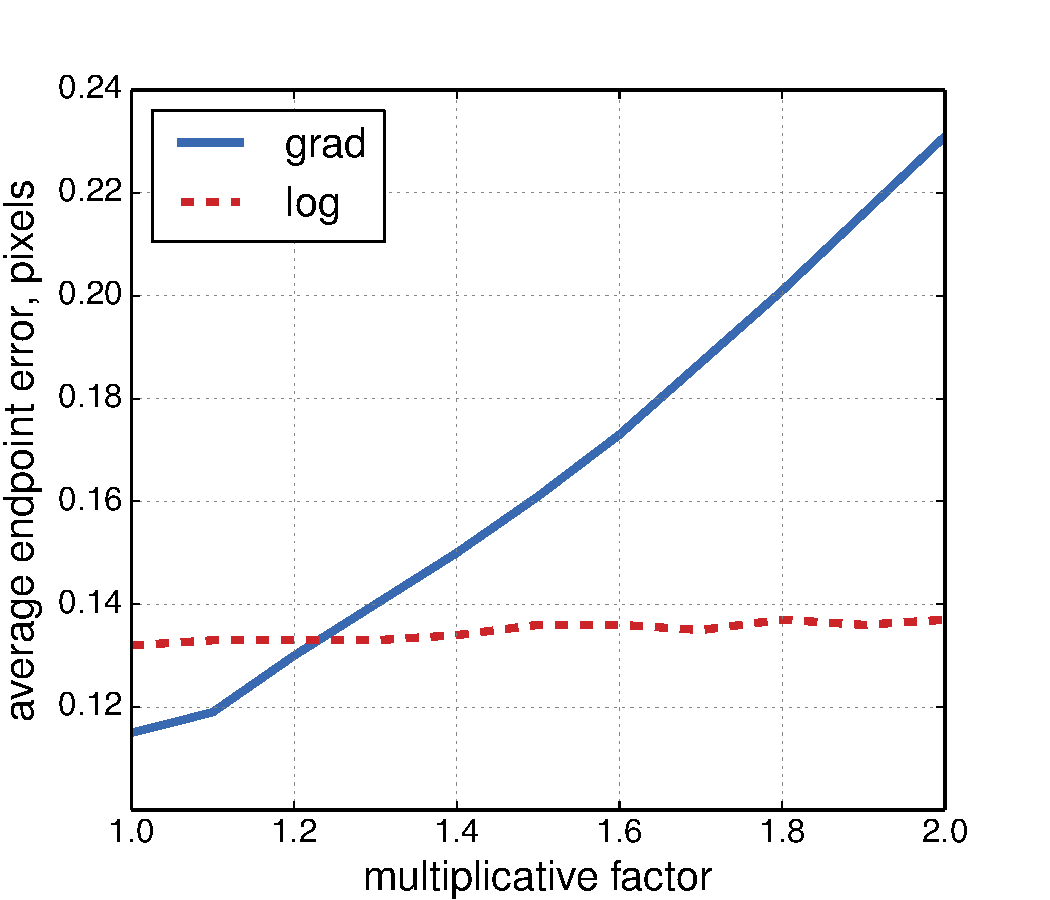
\includegraphics[width=0.45\textwidth]{figures/exp_mult_factor.pdf} 
  }  
  \caption{Comparison of gradient constancy assumption and log derivatives data terms for different values of multiplicative factor. Log-based data terms are robust under multiplicative brightness changes for all scaling factors.}
  \label{fig:exp_bright_mult_factor}
\end{figure*} 

From the evaluation of data terms and the experiment on the influence of multiplicative factor we can make the following conclusions:

\begin{itemize}

\item \textit{Gradient constancy assumption is the best data constraint for additive illumination changes}. This performance of gradient-based constancy assumption is not surprising, since derivatives are invariant w.r.t. global additive grey value changes. However, such situation is not realistic for X-ray imaging scenarios. For this reason, a performance of data terms on additive brightness change has little value for practical use on X-ray data.     

\item \textit{Log-derivatives based data term is robust with respect to multiplicative brightness changes}. Transformation of image data into logarithmic scale helps to overcome problems with multiplicative brightness changes. Log-derivatives based data term shows significantly better results in comparison with other data terms.

\item \textit{Log-derivatives based data term outperforms gradient data term only for large values of multiplicative factor}. The performance comparison of gradient-based and log-derivatives based constancy assumptions on various multiplicative factors (see Figure \ref{fig:exp_bright_mult_factor}) reveals, that the log-based constancy assumption starts to outperform the gradient constancy assumption for multiplicative factors greater than 1.2. It is important to note, that the brightness changes equivalent to multiplication by a factor greater than 1.5 are unlikely during image acquisition for a stable and well-adjusted imaging setup. However, if it is the case, then the log-based image derivatives data term is a suitable constancy assumption.  

\item \textit{Data preprocessing of initial image data significantly improves robustness against artifacts related to changing brightness conditions}. In the previous Section \ref{experiment_nonuniform_brightness} we evaluated and discussed the usefulness of a non-uniform brightness correction. In this section we compare the preprocessing approach with a model, which employs advanced data terms designed to provide robustness against such kind of conditions. From the quantitative results presented in Table \ref{tab:exp_bright_data_terms} one can observe, that preprocessing approach provides a good general performance. It gives similar results with the gradient constancy assumption on the multiplicative change dataset and outperforms all data terms for patterns "Spot" and "Strips". We want to emphasize that such kind of brightness change conditions are more physically relevant and more frequently occurring for the real life X-ray imaging experiments, then a global additive or strong multiplicative brightness changes.
\end{itemize}


% Table generated by Excel2LaTeX from sheet 'Sheet1'
\begin{table}[ht] \scriptsize
  \centering
  \caption{Performance of non-uniform brightness correction on \rub dataset. Four brightness patterns are used for the evaluation: additive (+30), multiplicative ($\times 1.5$), pattern \textit{"Spot"}, pattern \textit{"Stripes"}. Method: \textit{baseline}, data term = $\lbrace \text{grey}, \text{grey + Gaussian leveling}, \text{gradient}, \text{log-based derivatives}  \rbrace$, optimized $\sigma$ in the range $[0.15 .. 1.5]$, optimized $\alpha$ in the range $[0.005 .. 150]$. }
    \begin{tabular}{rrcrr}
    \toprule
    \multicolumn{1}{c}{brightness} & \multicolumn{1}{c}{data term} & \multicolumn{3}{c}{error} \\
    \midrule
          &       & \textit{all} & \multicolumn{1}{c}{\textit{disc}} & \multicolumn{1}{c}{\textit{untext}} \\
          \midrule   
          \midrule        
    \multicolumn{1}{l}{\multirow{4}[2]{*}{additive}} & \multicolumn{1}{l}{grey} & 1.143 & \multicolumn{1}{c}{1.17} & \multicolumn{1}{c}{1.056} \\
          & \multicolumn{1}{l}{filter + grey} & 0.128 & \multicolumn{1}{c}{0.581} & \multicolumn{1}{c}{0.089} \\
          & \multicolumn{1}{l}{grad} & \textbf{0.117} & \multicolumn{1}{c}{\textbf{0.543}} & \multicolumn{1}{c}{\textbf{0.084}} \\
          & \multicolumn{1}{l}{log} & 0.172 & \multicolumn{1}{c}{0.643} & \multicolumn{1}{c}{0.152} \\
          \midrule
    \multicolumn{1}{l}{\multirow{4}[2]{*}{multiplicative}} & \multicolumn{1}{l}{grey} & 1.212 & \multicolumn{1}{c}{1.204} & \multicolumn{1}{c}{1.12} \\
          & \multicolumn{1}{l}{filter + grey} & 0.162 & \multicolumn{1}{c}{0.613} & \multicolumn{1}{c}{0.103} \\
          & \multicolumn{1}{l}{grad} & 0.161 & \multicolumn{1}{c}{0.685} & \multicolumn{1}{c}{\textbf{0.09}} \\
          & \multicolumn{1}{l}{log} & \textbf{0.136} & \multicolumn{1}{c}{\textbf{0.554}} & \multicolumn{1}{c}{0.105} \\
          \midrule
    \multicolumn{1}{l}{\multirow{4}[2]{*}{\textit{"Spot"}}} & \multicolumn{1}{l}{grey} & 1.238 & \multicolumn{1}{c}{1.219} & \multicolumn{1}{c}{1.113} \\
          & \multicolumn{1}{l}{filter + grey} & \textbf{0.128} & \multicolumn{1}{c}{0.581} & \multicolumn{1}{c}{\textbf{0.088}} \\
          & \multicolumn{1}{l}{grad} & 0.129 & \multicolumn{1}{c}{\textbf{0.562}} & \multicolumn{1}{c}{0.099} \\
          & \multicolumn{1}{l}{log} & 0.221 & \multicolumn{1}{c}{0.723} & \multicolumn{1}{c}{0.224} \\
          \midrule
    \multicolumn{1}{l}{\multirow{4}[1]{*}{\textit{"Stripes"}}} & \multicolumn{1}{l}{grey} & 0.979 & \multicolumn{1}{c}{1.144} & \multicolumn{1}{c}{0.807} \\
          & \multicolumn{1}{l}{filter + grey} & \textbf{0.132} & \multicolumn{1}{c}{\textbf{0.584}} & \multicolumn{1}{c}{\textbf{0.093}} \\
          & \multicolumn{1}{l}{grad} & 0.153 & \multicolumn{1}{c}{0.594} & \multicolumn{1}{c}{0.118} \\
          & \multicolumn{1}{l}{log} & 0.242 & \multicolumn{1}{c}{0.748} & \multicolumn{1}{c}{0.197} \\
    \bottomrule
    \end{tabular}%
  \label{tab:exp_bright_data_terms}%
\end{table}%




\subsubsection{Experiment: Robust data term for low-contrast data}
\label{experiment_robust_data_term_low_contrast}

In this experiment we check the influence of robustification of data terms for low-contrast data. Since low-contrast data is characterized by small values of image derivatives, this might affect the computation of a motion tensor. For such situation the quadratic penalization of a data constancy assumption might be beneficial, since it provides more sensitivity to deviations from constancy assumptions.  In this experiment we test this hypothesis. For the evaluation we use both the grey value and the gradient value constancy assumptions.
The quantitative comparison between the original (quadratic) and the robust penalizer functions of the data term on low-contrast data is shown in Table \ref{tab:exp_robust_contrast}.
 


% Table generated by Excel2LaTeX from sheet 'result'
\begin{table}[ht] \scriptsize
  \centering
  \caption{Comparison of original (quadratic) and robust data term for low-contrast data. Contrast level of $C$ = 100\%, 50\%, 25\%, 12.5\% is used to simulate low-contrast data. Method: \textit{baseline}, model = $\lbrace \text{original}, \text{robust} \rbrace$, $\sigma=0.15$, optimized $\alpha$ in the range $[0.1 .. 10]$.}
    \begin{tabular}{crrcrr}
    \toprule
    \multicolumn{1}{c}{contrast} & \multicolumn{1}{c}{data} & \multicolumn{1}{c}{model} & \multicolumn{3}{c}{error} \\
    \midrule
          &       &       & \textit{all} & \multicolumn{1}{c}{\textit{disc}} & \multicolumn{1}{c}{\textit{untext}} \\
          \midrule
          \midrule
          
    \multicolumn{1}{r}{\multirow{4}[0]{*}{100\%}} & \multicolumn{1}{r}{\multirow{2}[0]{*}{grey}} & \multicolumn{1}{l}{original} & 0.169 & \multicolumn{1}{c}{0.628} & \multicolumn{1}{c}{0.131} \\
          &       & \multicolumn{1}{l}{robust} & \textbf{0.155} & \multicolumn{1}{c}{\textbf{0.61}} & \multicolumn{1}{c}{\textbf{0.128}} \\
          & \multicolumn{1}{r}{\multirow{2}[0]{*}{grad}} & \multicolumn{1}{l}{original} & 0.139 & \multicolumn{1}{c}{0.565} & \multicolumn{1}{c}{0.089} \\
          &       & \multicolumn{1}{l}{robust} & \textbf{0.11} & \multicolumn{1}{c}{\textbf{0.524}} & \multicolumn{1}{c}{\textbf{0.075}} \\
          \midrule
          
    \multicolumn{1}{r}{\multirow{4}[0]{*}{50\%}} & \multicolumn{1}{r}{\multirow{2}[0]{*}{grey}} & \multicolumn{1}{l}{original} & 0.169 & \multicolumn{1}{c}{0.629} & \multicolumn{1}{c}{\textbf{0.128}} \\
          &       & \multicolumn{1}{l}{robust} & \textbf{0.165} & \multicolumn{1}{c}{\textbf{0.612}} & \multicolumn{1}{c}{0.147} \\
          & \multicolumn{1}{r}{\multirow{2}[0]{*}{grad}} & \multicolumn{1}{c}{original} & 0.141 & \multicolumn{1}{c}{0.567} & \multicolumn{1}{c}{\textbf{0.091}} \\
          &       & \multicolumn{1}{l}{robust} & \textbf{0.121} & \multicolumn{1}{c}{\textbf{0.535}} & \multicolumn{1}{c}{0.094} \\
          \midrule
    \multicolumn{1}{r}{\multirow{4}[0]{*}{25\%}} & \multicolumn{1}{r}{\multirow{2}[0]{*}{grey}} & \multicolumn{1}{l}{original} & \textbf{0.169} & \multicolumn{1}{c}{0.63} & \multicolumn{1}{c}{\textbf{0.125}} \\
          &       & \multicolumn{1}{l}{robust} & 0.184 & \multicolumn{1}{c}{\textbf{0.629}} & \multicolumn{1}{c}{0.158} \\        
          
          & \multicolumn{1}{r}{\multirow{2}[0]{*}{grad}} & \multicolumn{1}{l}{original} & 0.14  & \multicolumn{1}{c}{0.57} & \multicolumn{1}{c}{\textbf{0.096}} \\
          &       & \multicolumn{1}{l}{robust} & \textbf{0.128} & \multicolumn{1}{c}{\textbf{0.549}} & \multicolumn{1}{c}{0.112} \\
          \midrule
    \multicolumn{1}{r}{\multirow{4}[0]{*}{12.5\%}} & \multicolumn{1}{r}{\multirow{2}[0]{*}{grey}} & \multicolumn{1}{l}{original} & \textbf{0.171} & \multicolumn{1}{c}{\textbf{0.634}} & \multicolumn{1}{c}{\textbf{0.138}} \\
          &       & \multicolumn{1}{l}{robust} & 0.219 & \multicolumn{1}{c}{0.654} & \multicolumn{1}{c}{0.18} \\
          & \multicolumn{1}{r}{\multirow{2}[0]{*}{grad}} & \multicolumn{1}{l}{original} & \textbf{0.153} & \multicolumn{1}{c}{0.585} & \multicolumn{1}{c}{\textbf{0.131}} \\
          &       & \multicolumn{1}{l}{robust} & 0.154 & \multicolumn{1}{c}{\textbf{0.573}} & \multicolumn{1}{c}{0.144} \\
    \bottomrule
    \end{tabular}%
  \label{tab:exp_robust_contrast}%
\end{table}%

Results of quantitative comparison of both data terms are:
\begin{itemize}
	\item \textit{For low-contrast image data the robust data term performs worse than the original (quadratic) data term}. From the performance analysis of robust data terms (both the grey value and the gradient value constancy assumptions), one may observe that the robust setting is not useful for all contrast levels. Starting from a contrast level of $C$ = 25\% the grey value constancy assumption provides worse results and starting from a level 12.5\% gradient constancy assumption in a robust setting no longer gives better results.   
	    
	\item \textit{Gradient constancy assumption outperforms the grey value constancy assumption in a robust setting for low-contrast data}. As it was already discussed in the previous experiment, the gradient constancy assumption is more suited for low-contrast data, since it is more sensitive to vanishing image gradients (as a result of contrast degradation). The same holds for a model using the gradient based data term in a robust setting. However, when the contrast drops down to 12.5\% both data terms in a robust setting provide worse result in comparison to a simple data term. Therefore, we conclude that for low-contrast image data the original (quadratic) data term should be employed or, alternatively, one may try to enhance the contrast using techniques presented in Section \ref{contrast_enhancement} and examined in the experimental Section \ref{experiment_local_contrast}.
	
%	 We discuss this aspect in the experimental section\ref{experiment_robust_data_term_noise}.  
	

\end{itemize}

% -----------------------------------------------------------
%%
%%
%AE: Comment 1) Not related to artifacts (as contrast and outliers) 2) Not tested on Poisson noise, which could resemble more "artifact-like" noise. It also could be that aonly Gaussian presmoothing helped to cope with noise, when robust settings somehow were less optimal. [SKIP???]
%%
%%
% -----------------------------------------------------------
 
%\subsubsection{Experiment: Robust data term for noisy data}
%\label{experiment_robust_data_term_noise}
%
%In this section we check the performance of a robust data term on noisy data.
%In general, robust setting should be advantageous in presence of image artifacts and data outliers. However, the performance on large scale noise is also interesting.  For evaluation we have use use Gaussian noise model and use \rub dataset.  The results are shown in Table \ref{tab:exp_robust_noise_rub}.
%
%% Table generated by Excel2LaTeX from sheet 'results'
%\begin{table}[ht] \footnotesize
%  \centering
%  \caption{Comparison of original (quadratic) and robust data term for noisy data.  \textit{Gaussian Noise} with zero mean value and standard deviation values of $\sigma$ = 5, 10, 20 was added. Method: \textit{baseline}, data term = $\lbrace \text{grey value}, \text{gradient value} \rbrace$, model = $\lbrace \text{original}, \text{robust} \rbrace$, $\sigma=0.15$,  optimized $\alpha$ in the range $\alpha=[0.1 .. 10]$.}
%    \begin{tabular}{rrrcrr}
%    \toprule
%    \multicolumn{1}{c}{noise} & \multicolumn{1}{c}{data} & \multicolumn{1}{c}{model} & \multicolumn{3}{c}{error} \\
%    \midrule
%          &       &       & \textit{all} & \multicolumn{1}{c}{\textit{disc}} & \multicolumn{1}{c}{\textit{untext}} \\
%          \midrule
%    \multicolumn{1}{r}{\multirow{4}[0]{*}{$\sigma$=0}} & \multicolumn{1}{r}{\multirow{2}[0]{*}{grey}} & original & 0.169 & \multicolumn{1}{c}{0.631} & \multicolumn{1}{c}{0.129} \\
%          &       & robust & \textbf{0.157} & \multicolumn{1}{c}{\textbf{0.615}} & \multicolumn{1}{c}{\textbf{0.129}} \\
%          & \multicolumn{1}{r}{\multirow{2}[0]{*}{grad}} & original & 0.139 & \multicolumn{1}{c}{0.569} & \multicolumn{1}{c}{0.089} \\
%          &       & robust & \textbf{0.11} & \multicolumn{1}{c}{\textbf{0.526}} & \multicolumn{1}{c}{\textbf{0.073}} \\
%          \midrule
%    \multicolumn{1}{r}{\multirow{4}[0]{*}{$\sigma$=5}} & \multicolumn{1}{r}{\multirow{2}[0]{*}{grey}} & original & \textbf{0.245} & \multicolumn{1}{c}{\textbf{0.707}} & \multicolumn{1}{c}{\textbf{0.23}} \\
%          &       & robust & 0.256 & \multicolumn{1}{c}{0.718} & \multicolumn{1}{c}{0.252} \\
%
%          & \multicolumn{1}{r}{\multirow{2}[0]{*}{grad}} & original & 0.245 & \multicolumn{1}{c}{0.699} & \multicolumn{1}{c}{0.251} \\
%          &       & robust & \textbf{0.233} & \multicolumn{1}{c}{\textbf{0.689}} & \multicolumn{1}{c}{\textbf{0.241}} \\
%          \midrule
%    \multicolumn{1}{r}{\multirow{4}[0]{*}{$\sigma$=10}} & \multicolumn{1}{r}{\multirow{2}[0]{*}{grey}} & original & \textbf{0.335} & \multicolumn{1}{c}{\textbf{0.768}} & \multicolumn{1}{c}{\textbf{0.326}} \\
%          &       & robust & 0.342 & \multicolumn{1}{c}{0.773} & \multicolumn{1}{c}{0.352} \\
%          & \multicolumn{1}{r}{\multirow{2}[0]{*}{grad}} & original & 0.345 & \multicolumn{1}{c}{0.778} & \multicolumn{1}{c}{0.37} \\
%          &       & robust & \textbf{0.33} & \multicolumn{1}{c}{\textbf{0.767}} & \multicolumn{1}{c}{\textbf{0.346}} \\
%          \midrule
%    \multicolumn{1}{r}{\multirow{4}[0]{*}{$\sigma$=20}} & \multicolumn{1}{r}{\multirow{2}[0]{*}{grey}} & original & \textbf{0.46} & \multicolumn{1}{c}{\textbf{0.851}} & \multicolumn{1}{c}{\textbf{0.546}} \\
%          &       & robust & 0.472 & \multicolumn{1}{c}{0.858} & \multicolumn{1}{c}{0.563} \\
%          & \multicolumn{1}{r}{\multirow{2}[0]{*}{grad}} & original & 0.479 & \multicolumn{1}{c}{0.877} & \multicolumn{1}{c}{0.565} \\
%          &       & robust & \textbf{0.462} & \multicolumn{1}{c}{\textbf{0.866}} & \multicolumn{1}{c}{\textbf{0.545}} \\
%    \bottomrule
%    \end{tabular}%
%  \label{tab:exp_robust_noise_rub}%
%\end{table}%
%
%Results of performance evaluation are:
%\begin{itemize}
%	\item \textit{Flow median filtering significantly improves optical flow result}. \change{ Not useful for grey value: for all noise levels, robust data term gives worse results. Since gradient constancy assumption is sensitive to noise, robust settings allows to improve the results.}
%\end{itemize}

	

\subsubsection{Experiment: Robust data term for images with artifacts}
\label{experiment_robust_data_term_artifacts}


In this section we test the performance of robust data terms on image data with artifacts. In the literature, the use of robust data term is well-studied for the original data containing natural artifacts, such as occlusions  \cite{Black96, Sun10, Middl, HarmonyFlow}.
An important addition of our study is that we introduce another structures, which aim to simulate artifacts frequently occurring for the real X-ray data. We control the placement of such artifacts and  regulate their effect by varying their thickness. Moreover, we check the performance of optical flow computation in the regions around the artifact structures (denoted as \textit{outliers}). 


Results of quantitative evaluation of the robust data term on different amounts of artifacts on the example of a grey value constancy assumption are shown in Table \ref{tab:exp_robust_artifacts}.


% Table generated by Excel2LaTeX from sheet 'Sheet1'
\begin{table}[ht] \scriptsize
  \centering
  \caption{Comparison of original (quadratic) and robust data term using grey value constancy assumption on images with data artifacts. Artifact structures with thickness of  $A$ = 0 (no artifacts), 1, 2, 3 pixels are added to original images to simulate data outliers. Method: \textit{baseline}, data term = $\lbrace \text{original}, \text{robust} \rbrace$, optimized $\sigma$ in the range $[0.15 .. 2.0]$,  optimized $\alpha$ in the range $[1.0 .. 40]$. }
    \begin{tabular}{rrcrrr}
    \toprule
    \multicolumn{1}{c}{artifacts} & \multicolumn{1}{c}{model} & \multicolumn{4}{c}{error} \\
    \midrule
          &       & \textit{all} & \multicolumn{1}{c}{\textit{disc}} & \multicolumn{1}{c}{\textit{untext}} & \multicolumn{1}{c}{\textit{outliers}} \\        
          \midrule
          \midrule       
    \multicolumn{1}{l}{\multirow{2}[0]{*}{$A_0$}} & \multicolumn{1}{l}{original} & 0.166 & \multicolumn{1}{c}{0.632} & \multicolumn{1}{c}{\textbf{0.127}} & \multicolumn{1}{c}{0.156} \\
          & \multicolumn{1}{l}{robust} & \textbf{0.157} & \multicolumn{1}{c}{\textbf{0.617}} & \multicolumn{1}{c}{0.129} & \multicolumn{1}{c}{\textbf{0.152}} \\
          \midrule
          
    \multicolumn{1}{l}{\multirow{2}[0]{*}{$A_1$}} & \multicolumn{1}{l}{original} & 0.294 & \multicolumn{1}{c}{0.803} & \multicolumn{1}{c}{0.302} & \multicolumn{1}{c}{1.04} \\
          & \multicolumn{1}{l}{robust} & \textbf{0.173} & \multicolumn{1}{c}{\textbf{0.645}} & \multicolumn{1}{c}{\textbf{0.157}} & \multicolumn{1}{c}{\textbf{0.217}} \\
          
          \midrule
    \multicolumn{1}{l}{\multirow{2}[0]{*}{$A_2$}} & \multicolumn{1}{l}{original} & 0.495 & \multicolumn{1}{c}{0.924} & \multicolumn{1}{c}{0.586} & \multicolumn{1}{c}{2.527} \\
          & \multicolumn{1}{l}{robust} & \textbf{0.221} & \multicolumn{1}{c}{\textbf{0.708}} & \multicolumn{1}{c}{\textbf{0.235}} & \multicolumn{1}{c}{\textbf{0.3}} \\
          
          \midrule
    \multicolumn{1}{l}{\multirow{2}[0]{*}{$A_3$}} & \multicolumn{1}{l}{original} & 0.694 & \multicolumn{1}{c}{1.142} & \multicolumn{1}{c}{0.797} & \multicolumn{1}{c}{3.915} \\
          & \multicolumn{1}{l}{robust} & \textbf{0.263} & \multicolumn{1}{c}{\textbf{0.734}} & \multicolumn{1}{c}{\textbf{0.29}} & \multicolumn{1}{c}{\textbf{0.328}} \\
    \bottomrule
    \end{tabular}%
  \label{tab:exp_robust_artifacts}%
\end{table}%

From the  performance evaluation we conclude that:
\begin{itemize}
	\item \textit{Robust data term significantly improves optical flow results in the presence of image artifacts}. As it was expected from the result of previous work, robust data terms  significantly improve the accuracy of optical flow. The performance improvement is especially remarkable in the \textit{outliers} regions. With the increased amount of artifacts the importance of robust data term becomes even more prominent. 
\end{itemize}


\subsubsection{Experiment: Flow median filtering}
\label{exp_flow_median}

We proceed with the experiment to test the performance of a median filtering of the intermediate flow result (see Section \ref{flow_median}). In the work of \cite{Sun10, Sun14} the authors already shown that the intermediate flow filtering allows to significantly improve the accuracy of optical flow. For this reason we skip such evaluation and proceed with a more challenging datasets. We assess the median filtering procedure in the presence of more severe artifacts. For this purpose we use the same approach to distribute data artifacts as in Section \ref{experiment_robust_data_term_artifacts}. For each artifacts level we evaluate the performance of different mask sizes of the median filter. Moreover, we present evaluation results of the median filtering procedure on two image sequences - \rub and \hyd datasets, since these datasets represent scenes with different sizes of moving objects. For the evaluation we use a \textit{baseline} model (see Section \ref{baseline_method}), which includes the usage of a robust data term.

Qualitative results using color coding are shown in Figure \ref{fig:exp_median_filtering}. One can see the improved robustness of optical flow computation, especially in the regions around image artifacts (regions \textit{outliers} in experimental Table \ref{tab:exp_median_filtering})   

\newcommand{\imageSizeb}{0.33}

\begin{figure*}[!ht]
  \centerline{
    \mbox{\includegraphicslabeledw[scale=\imageSizeb]{figures/rub1_a_3.png}{a}}
    \mbox{\includegraphicslabeledw[scale=\imageSizeb]{figures/rub2_a_3.png}{b}}    
  }
%  \vspace{3pt}
%  \centerline{
%    \mbox{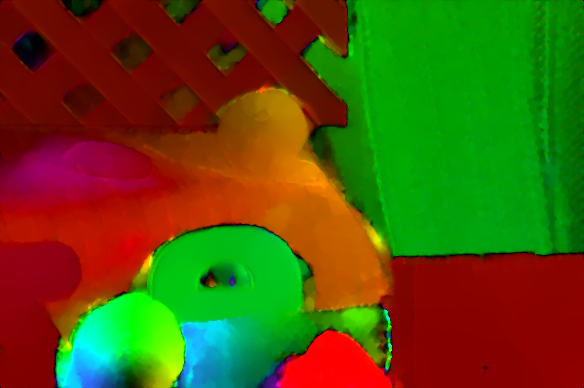
\includegraphics[scale=\imageSizeb]{figures/a0_nofilter.png}}
%    \mbox{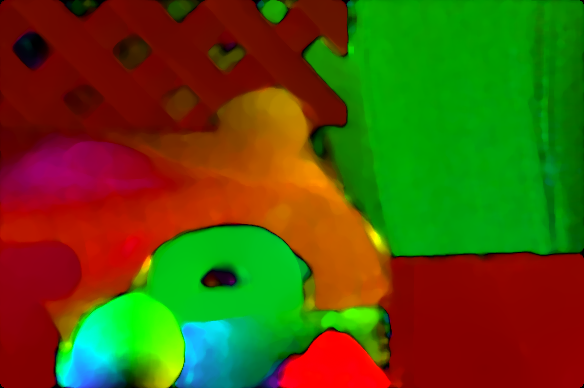
\includegraphics[scale=\imageSizeb]{figures/a0_m9.png}}
%  }
  \vspace{3pt}
  \centerline{
    \mbox{\includegraphicslabeledw[scale=\imageSizeb]{figures/a3_nofilter.png}{c}}
    \mbox{\includegraphicslabeledw[scale=\imageSizeb]{figures/a3_m9.png}{d}}
  }
  \caption[Modeling contrast]{Performance evaluation of flow median filtering on \rub dataset with image artifacts of thickness $A_3$. \textbf{(a)} First frame of degraded image sequence. \textbf{(b)} Second frame of the sequence. \textbf{(c)} \textit{Baseline} model \textit{without} median filtering. \textbf{(d)} Optical flow model \textit{with} median filtering with a spatial mask size $p=9$.  Flow errors due to image artifacts are significantly reduced. }
  \label{fig:exp_median_filtering}
\end{figure*}  


% Table generated by Excel2LaTeX from sheet 'Sheet1'
\begin{table}[h] \scriptsize
  \centering
  \caption{Performance evaluation of the flow intermediate filtering on images with data outliers. For the evaluation two image sequences are used: the \rub and the \hyd dataset, to check the performance of a median filtering for different sizes of moving objects.  Artifact structures with thickness of  $A$ = 0 (no artifacts), 1, 2, 3 pixels are added to the original images to simulate data outliers. Method: \textit{baseline}, size of a median filter mask $p$ = $\lbrace no filter, 3, 5, 7, 9 \rbrace$, optimized $\sigma$ in the range $[0.15 .. 2.0]$,  optimized $\alpha$ in the range $[1.0 .. 40]$.}
    \begin{tabular}{rrcrrrcrrr}
    \toprule
          &       & \multicolumn{4}{c}{\rub dataset} & \multicolumn{4}{c}{\hyd dataset} \\
    \midrule
           \multicolumn{1}{c}{artifacts} & \multicolumn{1}{c}{filter} & \multicolumn{4}{c}{error}     & \multicolumn{4}{c}{error} \\
          \midrule
          
          &       & \textit{all} & \multicolumn{1}{c}{\textit{disc}} & \multicolumn{1}{c}{\textit{untext}} & \multicolumn{1}{c}{\textit{outliers}} & \textit{all} & \multicolumn{1}{c}{\textit{disc}} & \multicolumn{1}{c}{\textit{untext}} & \multicolumn{1}{c}{\textit{outliers}} \\
          \midrule
          \midrule
    \multicolumn{1}{l}{\multirow{5}[1]{*}{$A_0$}} & \multicolumn{1}{c}{--} & 0.157 & \multicolumn{1}{c}{0.617} & \multicolumn{1}{c}{0.129} & \multicolumn{1}{c}{0.152} & 0.203 & \multicolumn{1}{c}{0.518} & \multicolumn{1}{c}{0.102} & \multicolumn{1}{c}{0.251} \\
    \multicolumn{1}{l}{} & \multicolumn{1}{l}{$p$ = 3} & 0.152 & \multicolumn{1}{c}{0.594} & \multicolumn{1}{c}{0.126} & \multicolumn{1}{c}{0.148} & \textbf{0.2} & \multicolumn{1}{c}{0.51} & \multicolumn{1}{c}{0.101} & \multicolumn{1}{c}{0.247} \\
    \multicolumn{1}{l}{} & \multicolumn{1}{l}{$p$ = 5} & 0.147 & \multicolumn{1}{c}{0.576} & \multicolumn{1}{c}{0.124} & \multicolumn{1}{c}{0.144} & 0.198 & \multicolumn{1}{c}{\textbf{0.504}} & \multicolumn{1}{c}{\textbf{0.1}} & \multicolumn{1}{c}{0.243} \\
    \multicolumn{1}{l}{} & \multicolumn{1}{l}{$p$ = 7} & 0.144 & \multicolumn{1}{c}{0.56} & \multicolumn{1}{c}{0.122} & \multicolumn{1}{c}{0.141} & 0.197 & \multicolumn{1}{c}{0.505} & \multicolumn{1}{c}{0.1} & \multicolumn{1}{c}{\textbf{0.242}} \\
    \multicolumn{1}{l}{} & \multicolumn{1}{l}{$p$ = 9} & \textbf{0.142} & \multicolumn{1}{c}{\textbf{0.556}} & \multicolumn{1}{c}{\textbf{0.121}} & \multicolumn{1}{c}{\textbf{0.14}} & 0.198 & \multicolumn{1}{c}{0.511} & \multicolumn{1}{c}{0.1} & \multicolumn{1}{c}{0.243} \\
    
    \midrule
    
    \multicolumn{1}{l}{\multirow{5}[2]{*}{$A_1$}} & \multicolumn{1}{c}{--} & 0.173 & \multicolumn{1}{c}{0.645} & \multicolumn{1}{c}{0.157} & \multicolumn{1}{c}{0.217} & 0.209 & \multicolumn{1}{c}{0.529} & \multicolumn{1}{c}{0.105} & \multicolumn{1}{c}{0.278} \\
    \multicolumn{1}{l}{} & \multicolumn{1}{l}{$p$ = 3} & 0.163 & \multicolumn{1}{c}{0.61} & \multicolumn{1}{c}{0.143} & \multicolumn{1}{c}{0.199} & 0.206 & \multicolumn{1}{c}{0.522} & \multicolumn{1}{c}{0.105} & \multicolumn{1}{c}{0.275} \\
    \multicolumn{1}{l}{} & \multicolumn{1}{l}{$p$ = 5} & 0.155 & \multicolumn{1}{c}{0.588} & \multicolumn{1}{c}{0.137} & \multicolumn{1}{c}{0.186} & 0.203 & \multicolumn{1}{c}{0.517} & \multicolumn{1}{c}{0.104} & \multicolumn{1}{c}{0.27} \\
    \multicolumn{1}{l}{} & \multicolumn{1}{l}{$p$ = 7} & 0.151 & \multicolumn{1}{c}{0.575} & \multicolumn{1}{c}{0.133} & \multicolumn{1}{c}{0.172} & \textbf{0.202} & \multicolumn{1}{c}{\textbf{0.516}} & \multicolumn{1}{c}{\textbf{0.103}} & \multicolumn{1}{c}{0.266} \\
    \multicolumn{1}{l}{} & \multicolumn{1}{l}{$p$ = 9} & \textbf{0.148} & \multicolumn{1}{c}{\textbf{0.567}} & \multicolumn{1}{c}{\textbf{0.13}} & \multicolumn{1}{c}{\textbf{0.161}} & 0.203 & \multicolumn{1}{c}{0.521} & \multicolumn{1}{c}{0.103} & \multicolumn{1}{c}{\textbf{0.264}} \\
    
    \midrule
    
    \multicolumn{1}{l}{\multirow{5}[2]{*}{$A_2$}} & \multicolumn{1}{c}{--} & 0.221 & \multicolumn{1}{c}{0.708} & \multicolumn{1}{c}{0.235} & \multicolumn{1}{c}{0.3} & 0.219 & \multicolumn{1}{c}{0.539} & \multicolumn{1}{c}{0.114} & \multicolumn{1}{c}{0.312} \\
    \multicolumn{1}{l}{} & \multicolumn{1}{l}{$p$ = 3} & 0.205 & \multicolumn{1}{c}{0.66} & \multicolumn{1}{c}{0.217} & \multicolumn{1}{c}{0.291} & 0.215 & \multicolumn{1}{c}{0.535} & \multicolumn{1}{c}{0.113} & \multicolumn{1}{c}{0.309} \\
    \multicolumn{1}{l}{} & \multicolumn{1}{l}{$p$ = 5} & 0.172 & \multicolumn{1}{c}{0.607} & \multicolumn{1}{c}{0.151} & \multicolumn{1}{c}{0.261} & 0.212 & \multicolumn{1}{c}{0.531} & \multicolumn{1}{c}{0.111} & \multicolumn{1}{c}{0.301} \\
    \multicolumn{1}{l}{} & \multicolumn{1}{l}{$p$ = 7} & 0.157 & \multicolumn{1}{c}{0.579} & \multicolumn{1}{c}{0.137} & \multicolumn{1}{c}{0.194} & \textbf{0.209} & \multicolumn{1}{c}{\textbf{0.529}} & \multicolumn{1}{c}{0.109} & \multicolumn{1}{c}{0.293} \\
    \multicolumn{1}{l}{} & \multicolumn{1}{l}{$p$ = 9} & \textbf{0.151} & \multicolumn{1}{c}{\textbf{0.57}} & \multicolumn{1}{c}{\textbf{0.132}} & \multicolumn{1}{c}{\textbf{0.172}} & 0.209 & \multicolumn{1}{c}{0.531} & \multicolumn{1}{c}{\textbf{0.108}} & \multicolumn{1}{c}{\textbf{0.288}} \\
    
    \midrule
    
    \multicolumn{1}{l}{\multirow{5}[1]{*}{$A_3$}} & \multicolumn{1}{c}{--} & 0.263 & \multicolumn{1}{c}{0.734} & \multicolumn{1}{c}{0.29} & \multicolumn{1}{c}{0.328} & 0.23  & \multicolumn{1}{c}{0.548} & \multicolumn{1}{c}{0.122} & \multicolumn{1}{c}{0.342} \\
    \multicolumn{1}{l}{} & \multicolumn{1}{l}{$p$ = 3} & 0.243 & \multicolumn{1}{c}{0.721} & \multicolumn{1}{c}{0.268} & \multicolumn{1}{c}{0.323} & 0.226 & \multicolumn{1}{c}{0.545} & \multicolumn{1}{c}{0.121} & \multicolumn{1}{c}{0.338} \\
    \multicolumn{1}{l}{} & \multicolumn{1}{l}{$p$ = 5} & 0.201 & \multicolumn{1}{c}{0.649} & \multicolumn{1}{c}{0.177} & \multicolumn{1}{c}{0.314} & 0.22  & \multicolumn{1}{c}{0.542} & \multicolumn{1}{c}{0.119} & \multicolumn{1}{c}{0.33} \\
    \multicolumn{1}{l}{} & \multicolumn{1}{l}{$p$ = 7} & 0.17  & \multicolumn{1}{c}{0.601} & \multicolumn{1}{c}{0.147} & \multicolumn{1}{c}{0.277} & 0.217 & \multicolumn{1}{c}{0.54} & \multicolumn{1}{c}{0.116} & \multicolumn{1}{c}{0.319} \\
    \multicolumn{1}{l}{} & \multicolumn{1}{l}{$p$ = 9} & \textbf{0.158} & \multicolumn{1}{c}{\textbf{0.582}} & \multicolumn{1}{c}{\textbf{0.139}} & \multicolumn{1}{c}{\textbf{0.211}} & \textbf{0.215} & \multicolumn{1}{c}{\textbf{0.54}} & \multicolumn{1}{c}{\textbf{0.114}} & \multicolumn{1}{c}{\textbf{0.309}} \\
    \bottomrule
    \end{tabular}%
  \label{tab:exp_median_filtering}%
\end{table}%

   
Quantitative results are presented in Table \ref{tab:exp_median_filtering}.
Evaluating the obtained results we can make the following conclusions:
\begin{itemize}
	\item \textit{Flow median filtering significantly improves optical flow results}.  As it was discussed earlier, in the case when artifacts are present in image data, errors in the flow estimation which originate already on coarse image scales are propagated via a warping step to the next computation level. Then, the incorrect flow serves as an initialization for optical flow estimation.  As a consequence, errors are accumulated during the incremental computation. The median filtering is an effective correction procedure to suppress flow errors already on earlier computation levels. 
	
	\item \textit{Large sizes of a median mask are useful to filter data outliers and improve overall accuracy of optical flow}. From the evaluation results on the \rub dataset we can conclude that large sizes of a median mask are useful to suppress data artifacts.   Surprisingly, it is also true for the original data with no additional artifact structures. In this case, the best results were given by a robust model with the median filtering with a spatial mask $p=9$.  With the increased amount of artifacts the importance of median filtering becomes even more prominent. As a conclusion - the stronger are the artifacts, the larger size of median mask is required.

	\item \textit{Optimum size of a median mask depends on the size of moving objects and the amount of flow discontinuities}. To compare the performance of a median filtering with different sizes of spatial mask we also evaluated the \hyd dataset. This dataset is characterized by small sizes of moving objects (plant leaves) and large amount of flow discontinuities (See Section \ref{synthetic_data}). As a result, for smaller amount of artifacts, the smaller size of a median mask is optimal (See Table \ref{tab:exp_median_filtering}). However, for the artifact level $A_3$ a median filter with a large mask size of $p=9$ provides the best results.
\end{itemize}

The evaluation of the flow median filtering procedure on the \mar dataset provides similar performance results (not shown here).







\subsubsection{Experiment: Data Refinement}
\label{exp_data_refinement}

In this experiment we evaluate the procedure of data refinement (see Section \ref{refinement}) as an additional correction step. It intends to improve the robustness of optical flow around strong data outliers. For the evaluation we use a \textit{baseline} model, which already includes a robust data term, but excludes other robust settings (e.g. the median filtering and the CLG approach). 

Analyzing qualitative results of optical flow shown in Figure \ref{fig:exp_refine} we can notice, that flow errors due to the strong image artifacts are almost completely eliminated. The visual quality is more appealing than the corresponding results using the median filtering approach (see Section \ref{exp_flow_median} and Figure \ref{fig:exp_median_filtering}).  Quantitative results are given in Table \ref{tab:exp_refine}. 

\newcommand{\imageSizec}{0.33}

\begin{figure*}[!ht]
  \centerline{
    \mbox{\includegraphicslabeledw[scale=\imageSizec]{figures/rub1_a_3.png}{a}}
    \mbox{\includegraphicslabeledw[scale=\imageSizec]{figures/rub2_a_3.png}{b}}    
  }
%  \vspace{3pt}
%  \centerline{
%    \mbox{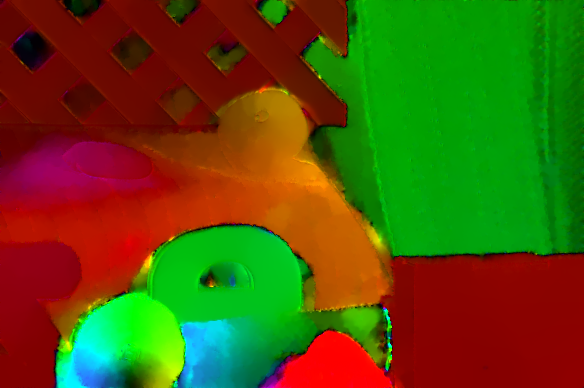
\includegraphics[scale=\imageSizec]{figures/ref_a0_noref.png}}
%    \mbox{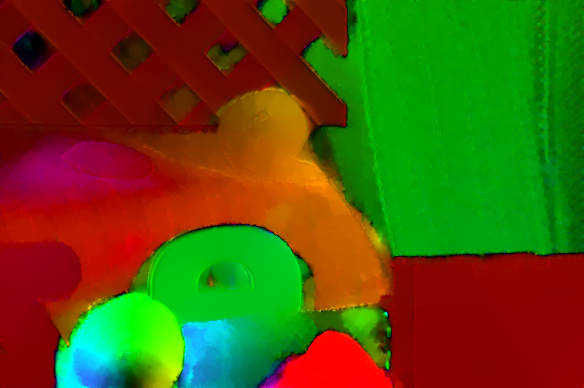
\includegraphics[scale=\imageSizec]{figures/ref_a0_ref.png}}
%  }
  \vspace{3pt}
  \centerline{
    \mbox{\includegraphicslabeledw[scale=\imageSizec]{figures/ref_a3_noref.png}{c}}
    \mbox{\includegraphicslabeledw[scale=\imageSizec]{figures/ref_a3_ref.png}{d}}
  }
  \caption[Modeling contrast]{{Performance evaluation of a data refinement procedure on the \rub dataset with image artifacts $A_3$ = 3 pixels. \textbf{(a)} First frame of degraded image sequence. \textbf{(b)} Second frame of the sequence. \textbf{(c)} \textit{Baseline} model \textit{without} data refinement. \textbf{(d)} Optical flow model \textit{with} data refinement. Flow errors due to image artifacts are almost completely eliminated.}}
  \label{fig:exp_refine}
\end{figure*}





% Table generated by Excel2LaTeX from sheet 'Sheet1'
\begin{table}[ht] \scriptsize
  \centering
  \caption{Performance evaluation of the data refinement procedure on images with data outliers. Artifact structures with thickness of $A$ = 0 (no artifacts), 1, 2, 3 pixels are added to the original images to simulate data outliers. Method: \textit{baseline}, model = $\lbrace \text{no refinement}, \text{with refinement} \rbrace$, optimized $\sigma$ in the range $[0.15 .. 2.0]$,  optimized $\alpha$ in the range $[1.0 .. 40]$.}
    \begin{tabular}{rrcrrr}
    \toprule
    \multicolumn{1}{c}{noise} & \multicolumn{1}{c}{model} & \multicolumn{3}{c}{error} &  \\
    \midrule
          &       & \textit{all} & \multicolumn{1}{c}{\textit{disc}} & \multicolumn{1}{c}{\textit{untext}} & \multicolumn{1}{c}{\textit{outliers}} \\
         \midrule
         \midrule
    \multicolumn{1}{r}{\multirow{2}[0]{*}{$A_0$}} & \multicolumn{1}{l}{no ref} & 0.157 & \multicolumn{1}{c}{0.617} & \multicolumn{1}{c}{0.129} & \multicolumn{1}{c}{0.152} \\
          & \multicolumn{1}{l}{refine} & \textbf{0.156} & \multicolumn{1}{c}{\textbf{0.591}} & \multicolumn{1}{c}{\textbf{0.131}} & \multicolumn{1}{c}{\textbf{0.156}} \\
          \midrule
    \multicolumn{1}{r}{\multirow{2}[0]{*}{$A_1$}} & \multicolumn{1}{l}{no ref} & 0.173 & \multicolumn{1}{c}{0.645} & \multicolumn{1}{c}{0.157} & \multicolumn{1}{c}{0.217} \\
          & \multicolumn{1}{l}{refine} & \textbf{0.163} & \multicolumn{1}{c}{\textbf{0.602}} & \multicolumn{1}{c}{\textbf{0.143}} & \multicolumn{1}{c}{\textbf{0.186}} \\
          \midrule
    \multicolumn{1}{r}{\multirow{2}[0]{*}{$A_2$}} & \multicolumn{1}{l}{no ref} & 0.221 & \multicolumn{1}{c}{0.708} & \multicolumn{1}{c}{0.235} & \multicolumn{1}{c}{0.3} \\
          & \multicolumn{1}{l}{refine} & \textbf{0.163} & \multicolumn{1}{c}{\textbf{0.603}} & \multicolumn{1}{c}{\textbf{0.144}} & \multicolumn{1}{c}{\textbf{0.183}} \\
          \midrule
    \multicolumn{1}{r}{\multirow{2}[0]{*}{$A_3$}} & \multicolumn{1}{l}{no ref} & 0.263 & \multicolumn{1}{c}{0.734} & \multicolumn{1}{c}{0.29} & \multicolumn{1}{c}{0.328} \\
          & \multicolumn{1}{l}{refine} & \textbf{0.168} & \multicolumn{1}{c}{\textbf{0.609}} & \multicolumn{1}{c}{\textbf{0.15}} & \multicolumn{1}{c}{\textbf{0.197}} \\
    \bottomrule
    \end{tabular}%
  \label{tab:exp_refine}%
\end{table}%


Results of our performance evaluation are:
\begin{itemize}
	\item \textit{Data refinement significantly improves the accuracy of optical flow computation in the presence of image artifacts}. Quantitative evaluation of optical flow model with data refinement reveals, that it is useful to weight down the contribution of a data term in the regions of strong image artifacts. As a result, accuracy of optical flow computation significantly improves.
	
	\item \textit{Data refinement outperforms the median filtering approach for smaller sizes of a median mask ($p < 9$)}. From both qualitative (see Figure \ref{fig:exp_refine}) and quantitative (see Table \ref{tab:exp_refine}) we can observe, that the data refinement approach outperforms the robust model based on the flow median filtering (see Figure \ref{fig:exp_median_filtering} and Table \ref{tab:exp_median_filtering}), except for the case when a larger mask of median filter is used ($p = 9$).
	
	\item \textit{Data refinement is especially useful within or around regions with strong data outliers}. When compared with median filtering approach using a large spatial mask size ($p = 9$) data refinement approach provided significantly better results in the \textit{outliers} regions, however was less accurate in other statistics regions (\textit{all}, \textit{disc}, \textit{untext}). A straightforward improvement would be a combination of both approaches into a single optical flow method. We evaluate this possibility in our final experiment (see Section \ref{models_comparison}).    
\end{itemize}

The evaluation of data refinement approach on \hyd and \mar datasets gives similar performance results (not shown here). 





%\subsubsection{[OPTIONAL] Experiment: Isotropic vs Anisotropic} 
%Isotropic vs Anisotropic smoothness \comment{In presence of noise and outliers, the structure is not preserved, so it could be no sense to use anisotropic setting}

%--------------------------------------------------------
\subsection{Experiments: Confidence Measures}
%--------------------------------------------------------
\label{exp_confidence_evaluation}

In this section we switch from the evaluation of different optical flow models to an important topic of automated confidence measures. This quantitative information could be obtained from the input image data and the computed flow field. As it was outlined earlier in our work, this topic is not sufficiently covered in the literature on optical flow. However, for analysis of real life data, especially in the case when it is diverse in its quality  and challenging to analyze, the topic of confidence measures is particularly important. With the appropriate use of such measures it is possible to evaluate the quality of the computed result and automatically optimize the model parameters. In the recent works of \cite{Sun10, HarmonyFlow} the authors demonstrated the benefits of such optimization.  

In this section we evaluate a number of confidence measures presented in Section \ref{confidence_measures}. We do not present the evaluation of such measures as the gradient-based approach and the motion uniqueness criteria in our final results, since these measures did not show an adequate performance. In the current evaluation we test the following confidence measures:
\begin{itemize}
	\item Data Constancy Error (see Section \ref{data_constancy_error})
    \item Forward-Backward Check (see Section \ref{forward_backward_check})
    \item Optimal Prediction Principle (see Section \ref{optimal_prediction_principle})
\end{itemize}

Additionally, we test the performance of confidence measures on different datasets (with varying amount of noise) and optical flow models. We use the \rub dataset and the following list of computation models:
\begin{itemize}
	\item Simple method $C_1$: Horn and Schunck method + multi-level computation 
	\item Advanced method $C_2$: Model $C_1$ + flow-driven smoothness  
	\item Baseline method $C_3$: $C_2$ + robust data term (see Section \ref{baseline_method}) 
	\item Robust method $C_4$: $C_3$ +  median filtering + combined local-global approach
    \item Noisy images $\sigma = 10$: we added \textit{Gaussian} noise 
     with zero mean and standard deviation values of $\sigma_n$ = 10 to the original \rub dataset. Method: robust method $C_4$ 
    \item Noisy images $\sigma = 20$: the same as the previous model, but with an increased level of noise ( $\sigma = 20$). Method: robust method $C_4$
    
\end{itemize}

For the evaluation we vary the value of the smoothness parameter $\alpha$ and compare distribution values of each confidence metric with the distribution of the average endpoint error provided by the ground truth result (AEE). Quantitative evaluation of confidence measures on a selected number of experimental models is presented in Figure \ref{fig:exp_confifance}. 


 \begin{figure*}[ht]
  \centerline{
    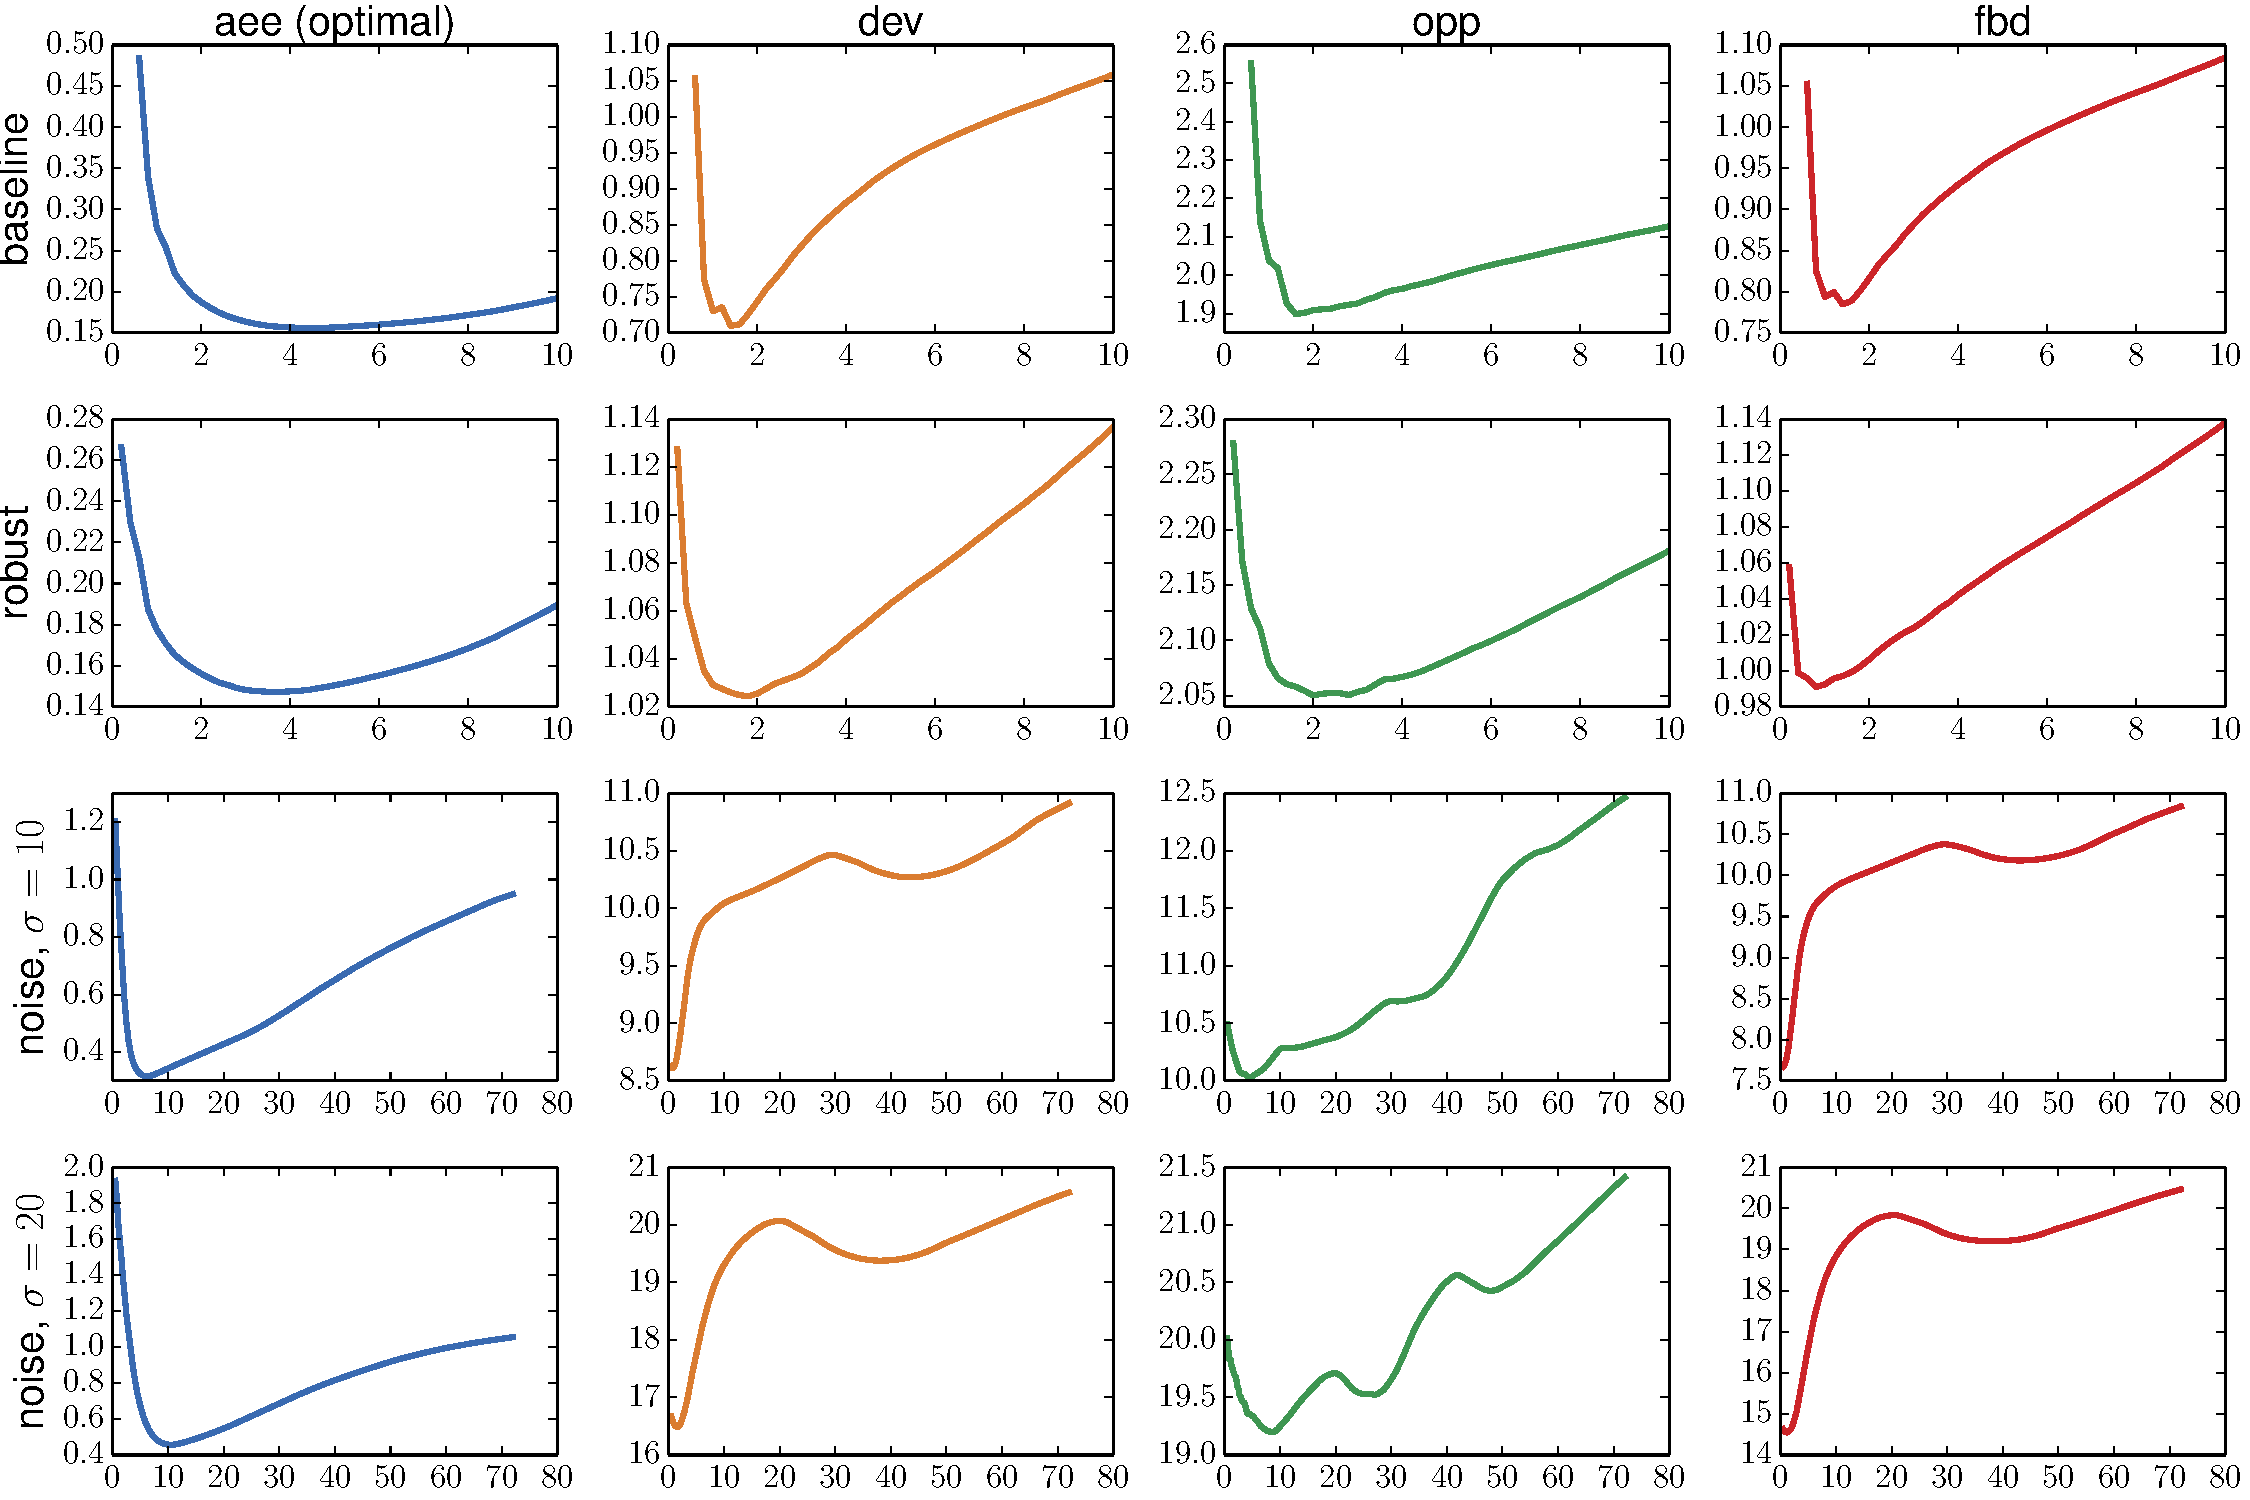
\includegraphics[width=0.97\textwidth]{figures/exp_confidance.pdf} 
  }  
  \caption{Comparison of confidence measures for different optical flow models on the \rub dataset. The value of the corresponding confidence metric is plotted over a list of varying smoothness parameters $\alpha$.  \textbf{First Row:}  Baseline method $C_3$.  \textbf{Second Row:}  Robust method $C_4$.  \textbf{Third Row:} Robust method $C_4$ on noisy images ($\sigma = 10$).  \textbf{Forth Row:}  Robust method $C_4$ on noisy images ($\sigma = 20$). \textbf{First Column:} Average endpoint error given by the comparison of the computed flow field with the ground truth result (\textit{aee}). \textbf{Second Column:} Data Constancy Error measure (\textit{dev}). \textbf{Third Column:} Confidence measure based on the Optimal Prediction Principle (\textit{opp}). \textbf{Forth Column:} Forward-Backward consistency check (\textit{fbd}).}
  \label{fig:exp_confifance}
\end{figure*} 

A summary of comparison between automatically selected smoothness parameter $\alpha$ using a confidence measure and the optimal parameter given by the ground truth is presented in Table \ref{tab:exp_confidance}.


% Table generated by Excel2LaTeX from sheet 'Sheet1'
\begin{table}[ht] \scriptsize
  \centering
  \caption{Comparison of confidence measures for optical flow models $C_1 - C_4$ on the original \rub dataset and datasets with noise. \textit{Gaussian} noise with zero mean value and standard deviation values of $\sigma_n$ = 10, 20 was added. The optimal value of a smoothness parameter $\alpha$ selected using the corresponding confidence measure approach is shown. Methods: Simple method $C_1$ (Horn and Schunck method + multi-level computation); Advanced method $C_2$ (Model $C_1$ + flow-driven smoothness);  Baseline method $C_3$ ($C_2$ + robust data term); Robust method $C_4$ ($C_3$ +  median filtering + combined local-global approach). No optimization of model parameters $\sigma, \rho$ was performed.}
    \begin{tabular}{rcccc}
    \toprule
       Method   & \textit{optim} & \textit{dev} & \textit{opp} & \textit{fbd} \\
    \midrule
    \midrule
    \multicolumn{1}{l}{Method $C_1$} & 55    & 15    & \textbf{24} & 15 \\
    \multicolumn{1}{l}{Method $C_2$} & 20    & 15    & \textbf{22} & 15 \\
    \multicolumn{1}{l}{Method $C_3$} & 4.4   & 1.4   & \textbf{1.6} & 1.4 \\
    \multicolumn{1}{l}{Method $C_4$} & 3.6   & 1.8   & \textbf{2} & 0.8 \\
    \multicolumn{1}{l}{Method $C_4$ + noise ($\sigma=$10)} & 6.1   & 0.7   & \textbf{4.5} & 0.5 \\
    \multicolumn{1}{l}{Method $C_4$ + noise ($\sigma=$20)} & 10.5  & 1.7   & \textbf{8.7} & 1.1 \\
    \bottomrule
    \end{tabular}%
  \label{tab:exp_confidance}%
\end{table}%

Results of performance evaluation are:
\begin{itemize}
	\item \textit{Confidence measure based on the Optimal Prediction Principle is more accurate to predict quality of optical flow computation}. Based on the evaluation of all optical flow models (see Table \ref{tab:exp_confidance}) we conclude that OPP measure gives the best results to describe the quality of the computed flow field in the case when ground truth result is not known.
	
	\item \textit{Performance of confidence measures depends on the optical flow model and input data}. Such measures as the Data Constancy Error (\textit{dev}) and Forward-Backward Check (\textit{fbd}) failed to provide optimal results. With an increase of noise this effect magnifies. Note, that we do not optimized other parameters, such as $\sigma$, to show the influence of an individual parameter. In general, all confidence measures performed less stable on the datasets with noise, which could potentially limit their application.   
	
	\item \textit{If a confidence measure based on the Optimal Prediction Principle cannot be applied due to violation of its assumptions the next optimal confidence measure is based on the Data Constancy Error}. This measure performed less accurate in comparison with OOP metric (see Table \ref{tab:exp_confidance}). However, this measure has a number of advantages: there are no assumptions about an image sequence and a motion model, except the ones incorporated in the data constancy assumption;  it is general and could be applied for any optical flow model.
\end{itemize}


%--------------------------------------------------------
\section{Models Comparison}
\label{models_comparison}
%--------------------------------------------------------


So far we have experimented on individual components of optical flow models. In this section we put all the successful model into a single technique.
We examine step by step how additional optical flow features improve the accuracy of results. We do not provide the performance analysis on the original data, because it does not comply with the purpose of this work, which is focused on a challenging X-ray data. Instead, we use a dataset with a simulated Poisson noise (P = 200) and substantial amount of image artifacts.  Starting from the simplest approach - the Horn and Schunck method we gradually include other optical flow features and end up with the most advanced and robust model.



For a shorter model notation we use the name of the previously introduced model and give names of additional features. The final model combines all the robust features. We evaluate the following optical flow models:
\begin{itemize}
	\item Model $M_1$: Classical Horn and Schunck model (see Section \ref{general_model})
	\item Model $M_2 = M_1$ + flow-driven smoothness term (see Section \ref{flow_driven})
    \item Model $M_3 = M_2$ + multi-level computation (see Section \ref{multilevel})
	\item Model $M_4 = M_3$ + robust data term (see Section \ref{robust})   
    \item Model $M_5 = M_4$ + combined local-global approach (CLG) (see Section \ref{clg})
    \item Model $M_6 = M_5$ + median filtering of an intermediate flow result
    \item Model $M_7 = M_6$ + data refinement step (see Section \ref{refinement}) using the forward-backward check method as a confidence map (see Section \ref{forward_backward_check})
\end{itemize}






% Table generated by Excel2LaTeX from sheet 'res'
\begin{table}[ht] \scriptsize
  \centering
  \caption{Comparison of optical flow models $M_1 - M_7$ on the \rub dataset with added noise and image artifacts. \textit{Poisson noise}: Mean value of Poisson random distribution $P$ = 200. Artifact structures with thickness of  $A$ = 2 pixels are added to original images to simulate data outliers. In addition to a common average enpoint error (AEE) we provide a robust statistics metric R1.0 (see Section \ref{error_statistics}), which helps to judge about qualitative performance. Method: according to model $M_i$, optimized $\rho$ in the range $[0.5 .. 2.0]$, optimized $\sigma$ in the range $[0.35 .. 2.5]$, optimized $\alpha$ in the range $[3.0 .. 2000]$.}
    \begin{tabular}{rcrrrcrrr}
    \toprule
    \multicolumn{1}{c}{model} & \multicolumn{4}{c}{AEE error} & \multicolumn{4}{c}{R1.0 statistics} \\
    \midrule
          & \textit{all} & \multicolumn{1}{c}{\textit{disc}} & \multicolumn{1}{c}{\textit{untext}} & \multicolumn{1}{c}{\textit{outliers}} & \textit{all} & \multicolumn{1}{c}{\textit{disc}} & \multicolumn{1}{c}{\textit{untext}} & \multicolumn{1}{c}{\textit{outliers}} \\
          \midrule
          \midrule
    \multicolumn{1}{l}{$M_1$ = HS} & 0.599 & \multicolumn{1}{c}{0.963} & \multicolumn{1}{c}{0.72} & \multicolumn{1}{c}{0.704} & 17.9  & \multicolumn{1}{c}{36.7} & \multicolumn{1}{c}{24.8} & \multicolumn{1}{c}{25.1} \\
    \multicolumn{1}{l}{$M_2 = M_1 + $ flow-driven} & 0.784 & \multicolumn{1}{c}{1.011} & \multicolumn{1}{c}{1.014} & \multicolumn{1}{c}{1.125} & 26.6  & \multicolumn{1}{c}{35} & \multicolumn{1}{c}{41.2} & \multicolumn{1}{c}{41.2} \\
    \multicolumn{1}{l}{$M_3 = M_2 + $ warping} & 0.51  & \multicolumn{1}{c}{0.904} & \multicolumn{1}{c}{0.637} & \multicolumn{1}{c}{0.745} & 13.1  & \multicolumn{1}{c}{31.8} & \multicolumn{1}{c}{13.5} & \multicolumn{1}{c}{18} \\
    \multicolumn{1}{l}{$M_4 = M_3 + $ robust data term} & 0.43  & \multicolumn{1}{c}{0.834} & \multicolumn{1}{c}{0.522} & \multicolumn{1}{c}{0.462} & 9.8   & \multicolumn{1}{c}{29.6} & \multicolumn{1}{c}{9.4} & \multicolumn{1}{c}{9.9} \\
    \multicolumn{1}{l}{$M_5 = M_4 + $ CLG} & 0.378 & \multicolumn{1}{c}{0.829} & \multicolumn{1}{c}{0.406} & \multicolumn{1}{c}{0.416} & 9.4   & \multicolumn{1}{c}{29.4} & \multicolumn{1}{c}{9} & \multicolumn{1}{c}{10.2} \\
    \multicolumn{1}{l}{$M_6 = M_5 + $ median filtering} & 0.376 & \multicolumn{1}{c}{0.82} & \multicolumn{1}{c}{0.395} & \multicolumn{1}{c}{0.409} & 9.1   & \multicolumn{1}{c}{28.3} & \multicolumn{1}{c}{8.9} & \multicolumn{1}{c}{9.7} \\
    \multicolumn{1}{l}{$M_7 = M_6 + $ refinement} & \textbf{0.353} & \multicolumn{1}{c}{\textbf{0.821}} & \multicolumn{1}{c}{\textbf{0.351}} & \multicolumn{1}{c}{\textbf{0.386}} & \textbf{8.8} & \multicolumn{1}{c}{\textbf{28.1}} & \multicolumn{1}{c}{\textbf{8.6}} & \multicolumn{1}{c}{\textbf{9.5}} \\
    \bottomrule
    \end{tabular}%
  \label{tab:exp_model_comp}%
\end{table}%

\newcommand{\imageSizea}{0.35}

\begin{figure*}[!ht]
	\centerline{
		\mbox{\includegraphicslabeledw[scale=\imageSizea]{figures/rub_art_1.png}{a}}
		\mbox{\includegraphicslabeledw[scale=\imageSizea]{figures/rub_art_2.png}{b}}    
	}
	\vspace{3pt}
	\centerline{
		\mbox{\includegraphicslabeledw[scale=\imageSizea]{figures/rub_gt.png}{c}}
		\mbox{\includegraphicslabeledw[scale=\imageSizea]{figures/models_comp_1_hs.png}{d}}
	}
	\vspace{3pt}
	\centerline{
		\mbox{\includegraphicslabeledw[scale=\imageSizea]{figures/models_comp_2_flow.png}{e}}
		\mbox{\includegraphicslabeledw[scale=\imageSizea]{figures/models_comp_3_warp.png}{f}}
	}
	\vspace{3pt}
	\centerline{
		\mbox{\includegraphicslabeledw[scale=\imageSizea]{figures/models_comp_5_clg.png}{g}}
		\mbox{\includegraphicslabeledw[scale=\imageSizea]{figures/models_comp_7_refine.png}{h}}
	}
	\caption[Modeling contrast]{Comparison of optical flow models $M_1 - M_7$ on the \rub dataset with added noise and image artifacts. \textbf{(a)} First frame of degraded image sequence. \textbf{(b)} Second frame of the sequence. \textbf{(c)} Ground truth result. \textbf{(d)} Model $M_1$: Classical Horn and Schunck. \textbf{(e)} Model $M_2 = M_1$ + flow-driven smoothness term. \textbf{(f)} Model $M_3 = M_2$ + multi-level computation. \textbf{(g)}  Model $M_5 = M_4$ + robust data term + combined local-global approach. \textbf{(h)} Model $M_7 = M_5$ + median filtering + data refinement step.}
	\label{fig:models_comparison}
\end{figure*}

Analyzing the results which are given in Figure \ref{fig:models_comparison} and the corresponding quantitative performance metrics from Table \ref{tab:exp_model_comp} we can make the following observations:
\begin{itemize}
	\item  As it was expected, the simplest optical flow model gives the worst accuracy. The flow magnitudes were not captured correctly, since no strategy to cope with large displacements were employed. The optimal model parameters are the large presmoothing parameter $\sigma$ and the large smoothness regularization parameter $\alpha$.  By oversmoothning the initial data this helped to reduce the influence of data outliers (see Figure \ref{fig:models_comparison}d).
	
	\item  An interesting aspect of our evaluation is that the flow-driven smoothness approach performed significantly worse then a simple method using the homogeneous regularization. Adaptive smoothness regularization was not sufficient to cope with data outliers (see Figure \ref{fig:models_comparison}e) and provide filling-in effect in homogeneous image regions (see Figure \ref{fig:models_comparison}e).  

	\item With the incorporation of a multi-level computation technique the flow in homogeneous regions is estimated correctly (see Figure \ref{fig:models_comparison}f). Moreover, the estimation of the magnitude of the flow field improves.
	
	\item The use of the combined local-global approach significantly improves the robustness of the optical flow method under noise and data artifacts (see Figure \ref{fig:models_comparison}g). 

	\item Addition of the median filtering of intermediate flow results between levels of a coarse-to-fine computation strategy and subsequent selective refinement of the data term weight according to the automated confidence measure further improves robustness against artifacts (see Figure \ref{fig:models_comparison}h).
		
\end{itemize}

To summarize, for all testing datasets with artifacts (Poisson noise $P=200$ and artifact structures $A_2$) we compare the performance of a \textit{baseline}  method $M_3$ (see Section \ref{baseline_method}) with a robust optical flow method $M_7$.
The quantitative comparison is presented in Table \ref{tab:exp_model_comp_3datasets} and qualitative visualization of computed flow fields is given in Figure \ref{fig:exp_model_comp_3datasets}.
For all dataset the robust model, designed for challenging X-ray data provides significantly better results as measured using the average endpoint error metric for the entire image.
   


% Table generated by Excel2LaTeX from sheet 'Sheet1'
\begin{table}[ht] \scriptsize
  \centering
  \caption{Comparison of optical flow models $M_3$ and $M_7$ on the \textit{RubberWhale}, \hyd and \mar  datasets with added noise and image artifacts. \textit{Poisson noise}: Mean value of Poisson random distribution $P$ = 200. Artifact structures with thickness of  $A$ = 2 pixels are added to the original images to simulate data outliers. Average endpoint error and Robust statistics are shown. Methods: according to models $M_3$ and $M_7$, optimized $\rho$ in the range $[0.5 .. 2.0]$, optimized $\sigma$ in the range $[0.35 .. 2.5]$, optimized $\alpha$ in the range $[3.0 .. 40]$.} 
    \begin{tabular}{rrcrrrcrrr}
    \toprule
          &       & \multicolumn{4}{c}{AEE error} & \multicolumn{4}{c}{R1.0 statistics} \\
    \midrule
          &       & \textit{all} & \multicolumn{1}{c}{\textit{disc}} & \multicolumn{1}{c}{\textit{untext}} & \multicolumn{1}{c}{\textit{outliers}} & \textit{all} & \multicolumn{1}{c}{\textit{disc}} & \multicolumn{1}{c}{\textit{untext}} & \multicolumn{1}{c}{\textit{outliers}} \\
          \midrule
          \midrule
    \multirow{2}[0]{*}{\rub} & baseline & 0.43  & \multicolumn{1}{c}{\textbf{0.834}} & \multicolumn{1}{c}{0.522} & \multicolumn{1}{c}{0.462} & 9.83  & \multicolumn{1}{c}{\textbf{29.59}} & \multicolumn{1}{c}{9.44} & \multicolumn{1}{c}{\textbf{9.93}} \\
          & robust & \textbf{0.353} & \multicolumn{1}{c}{0.845} & \multicolumn{1}{c}{\textbf{0.351}} & \multicolumn{1}{c}{\textbf{0.39}} & \textbf{9.1} & \multicolumn{1}{c}{30.26} & \multicolumn{1}{c}{\textbf{8.8}} & \multicolumn{1}{c}{10.2} \\
          \midrule
    \multirow{2}[0]{*}{\hyd} & baseline & 0.728 & \multicolumn{1}{c}{\textbf{0.63}} & \multicolumn{1}{c}{0.737} & \multicolumn{1}{c}{0.918} & 18.32 & \multicolumn{1}{c}{16.45} & \multicolumn{1}{c}{17.05} & \multicolumn{1}{c}{27.49} \\
          & robust & \textbf{0.343} & \multicolumn{1}{c}{0.632} & \multicolumn{1}{c}{\textbf{0.279}} & \multicolumn{1}{c}{\textbf{0.413}} & \textbf{5.84} & \multicolumn{1}{c}{\textbf{15.98}} & \multicolumn{1}{c}{\textbf{4.19}} & \multicolumn{1}{c}{\textbf{8.02}} \\
          \midrule
    \multirow{2}[0]{*}{\mar} & baseline & 0.077 & \multicolumn{1}{c}{\textbf{0.492}} & \multicolumn{1}{c}{0.054} & \multicolumn{1}{c}{0.096} & \textbf{0.29} & \multicolumn{1}{c}{\textbf{10.87}} & \multicolumn{1}{c}{0} & \multicolumn{1}{c}{\textbf{0.55}} \\
          & robust & \textbf{0.067} & \multicolumn{1}{c}{0.523} & \multicolumn{1}{c}{\textbf{0.051}} & \multicolumn{1}{c}{\textbf{0.086}} & 0.41  & \multicolumn{1}{c}{14.81} & \multicolumn{1}{c}{0} & \multicolumn{1}{c}{0.74} \\
    \bottomrule
    \end{tabular}%
  \label{tab:exp_model_comp_3datasets}%
\end{table}%



\newcommand{\imageSized}{0.27}
\newcommand{\imageSizee}{0.307}

\begin{figure*}[!ht]

  \centerline{
    \mbox{\includegraphicslabeledw[scale=\imageSized]{figures/rub_grounfTruth_bruhn_scale_2px.png}{a}}
    \mbox{\includegraphicslabeledw[scale=\imageSized]{figures/models_rub_basic.png}{b}}
    \mbox{\includegraphicslabeledw[scale=\imageSized]{figures/models_rub_robust.png}{c}}
  }
  \vspace{3pt}
  \centerline{
    \mbox{\includegraphicslabeledw[scale=\imageSized]{figures/hyd_groundTruth_bruhn_scale_2px.png}{d}}
    \mbox{\includegraphicslabeledw[scale=\imageSized]{figures/models_hyd_basic.png}{e}}
    \mbox{\includegraphicslabeledw[scale=\imageSized]{figures/models_hyd_robust.png}{f}}
  }
  \vspace{3pt}
  \centerline{
    \mbox{\includegraphicslabeledw[scale=\imageSizee]{figures/marble_groundTruth_bruhn_scale_2px.png}{g}}
    \mbox{\includegraphicslabeledw[scale=\imageSizee]{figures/models_mar_basic.png}{h}}
    \mbox{\includegraphicslabeledw[scale=\imageSizee]{figures/models_mar_robust.png}{i}}
  }
  \caption[Modeling contrast]{Comparison of advanced optical flow model $M_4$ and robust optical flow model $M_7$ on \rub dataset with added noise and image artifacts. \textbf{(a)} Ground truth flow result for the \rub dataset. \textbf{(b)} Flow field computed using $M_4$ optical flow model. \textbf{(c)} Flow field computed using the robust $M_7$ optical flow model. \textbf{(d)} Ground truth flow result for the \hyd dataset. \textbf{(e)} Flow field computed using $M_4$ optical flow model. \textbf{(f)} Flow field computed using the robust $M_7$ optical flow model. \textbf{(g)} Ground truth flow result for the \mar dataset. \textbf{(h)} Flow field computed using $M_4$ optical flow model. \textbf{(i)} Flow field computed using the robust $M_7$ optical flow model.}
  \label{fig:exp_model_comp_3datasets}
\end{figure*}



%\section{Experiments on Real Data}
%
%\comment{Skip? GT in not available anyway}
%Real dataset (Semi-solid alloys) using manual annotation.
%
%Figure. Getting GT for real data. Left: Original image. Middle left: Labeled 1, Middle right: Labeled 2, Right: GT flow field.


\newpage

\section{Evaluation Summary}
\label{experiments_summary}

In this section we provide a summary list of our quantitative experiments with synthetic data presented in the current chapter. We enlist all the conclusions as it is stated in the corresponding experimental section. This list of justified principles should serve us as a general reference for the choice of appropriate optical flow models and their parameters.    

\subsection*{Experiments: Noise}

\begin{itemize}
	\item Gradient constancy assumption with the robust setting provides good results for both Gaussian and Poisson noise models.
	    
	\item Higher order derivatives are sensitive to noise for the Gaussian, Poisson and Spike noise models. 
	
	\item Grey value constancy assumption is more robust for the Spike noise model.
	
	\item Grey value constancy assumption is more robust for the Poisson noise model in the regions of image discontinue.
	
	\item Integration of local information is useful to improve results on noisy data.
	
	\item Data normalization improves results on noisy data.
	    
	\item Data normalization approach outperforms the Combined Local-Global approach (CLG) on flow boundaries.   
	
	\item Data normalization can be further combined with the CLG approach to improve results.
\end{itemize}
	
\subsection*{Experiments: Preprocessing}

\begin{itemize}	
	\item Noise filtering of initial data can be helpful. 
	    
	\item For each noise model there is an optimal filtering procedure.
	
	\item Gaussian filtering is a simple and effective filtering procedure. 
	
	\item Gaussian filtering is useful to remove Poisson noise.

	\item Usefulness of Anisotropic diffusion filtering for complex noise scenarios.
		
	\item The appropriate choice of a filtering procedure and its parameters is crucial, however, a challenging task. 
\end{itemize}
	
\subsection*{Experiments: Artifacts}
\begin{itemize}	
	
	\item Brightness correction procedure significantly improves results of optical flow in the presence of brightness variations
	
	\item Multiplicative brightness change is the most complicated brightness change scenario.
	
	\item Contrast enhancement is not useful for noise-free images.
	
	\item Contrast enhancement could be helpful for low-contrast images with noise.
	
	\item Performance of contrast enhancement depends on the statistics of noise distribution.
	
	\item The contrast-to-noise ratio (CNR) is a crucial quality measure for analysis of X-ray data.
	
	\item Higher-order data terms provide better results for low-contrast images.
	
	\item Gradient value constancy assumption provides the best results for low-contrast data.
	
	\item Lower values of the smoothness parameter are required for low-contrast data.
	
	\item Gradient constancy assumption is the best data constraint for additive illumination changes.
	
	\item Log-derivatives based data term is robust with respect to multiplicative brightness changes.
	
	\item Log-derivatives based data term outperforms gradient data term only for large values of multiplicative factor.
	
	\item Data preprocessing of initial image data significantly improves robustness against artifacts related to changing brightness conditions.
	
	\item For low-contrast image data the robust data term performs worse than the original (quadratic) data term.
	
	\item Gradient constancy assumption outperforms the grey value constancy assumption in a robust setting for low-contrast data.
	
	\item Robust data term significantly improves optical flow results in the presence of image artifacts.
	
	\item Flow median filtering significantly improves optical flow results.
	
	\item Large sizes of a median mask are useful to filter data outliers and improve overall accuracy of optical flow.
	
	\item Optimum size of a median mask depends on the size of moving objects and the amount of flow discontinuities.
	
	\item Data refinement significantly improves the accuracy of optical flow computation in the presence of image artifacts.
	
	\item Data refinement outperforms the median filtering approach for smaller sizes of a median mask ($p < 9$).
	
	\item Data refinement is especially useful within or around regions with strong data outliers.
	
	
\end{itemize}
	
\subsection*{Experiments: Confidence Measures}


\begin{itemize}
	\item Confidence measure based on the Optimal Prediction Principle is more accurate to predict quality of optical flow computation.
	
	\item Performance of confidence measures depends on the optical flow model and input data. 
	
	\item If a confidence measure based on the Optimal Prediction Principle cannot be applied due to violation of its assumptions (linear motion, more then two frames available) the next optimal confidence measure is based on Data Constancy Error.
\end{itemize}




   


%\comment{Info from Secrets paper, in the similar manner}
%\comment{Make a table or block diagram of the best models, options, refer to experiments and previous work of \cite{Middl}, \cite{Secrets}, \cite{HarmonyFlow}}


